\documentclass{}
\usepackage{epsfig,amsmath,graphicx,cite,lmodern}
\usepackage{subfig}
\usepackage[utf8]{inputenc}

%allgemeine Formatangaben
\documentclass[
 a4paper, 										% Papierformat
 12pt,												% Schriftgröße
 ngerman, 										% für Umlaute, Silbentrennung etc.
 titlepage,										% es wird eine Titelseite verwendet
 bibliography=totoc,					% Literaturverzeichnis im Inhaltsverzeichnis aufführen
 listof=totoc,								% Verzeichnisse im Inhaltsverzeichnis aufführen
 twoside, 										% einseitiges Dokument
 captions=nooneline,					% einzeilige Gleitobjekttitel ohne Sonderbehandlung wie mehrzeilige Gleitobjekttitel behandeln
 numbers=noenddot,						% Überschriften-??Nummerierung ohne Punkt am Ende
 parskip=half,							% zwischen Absätzen wird eine halbe Zeile eingefügt
 ]{scrbook}

\usepackage[bindingoffset=10mm]{geometry}% Bindeverlust von 8mm einbeziehen

\newcommand{\titel}{Learning drinking patterns with Q-Learning and Feature Selection on an Ethereum Blockchain}
 			% einbinden von persönlichen Daten

% Anpassung an Landessprache
\usepackage[ngerman]{babel}
 
% Verwenden von Sonderzeichen und Silbentrennung
%\usepackage[latin1]{inputenc}	
%\usepackage[T1]{fontenc}
%\usepackage[ansinew]{inputenc}
%\usepackage[applemac]{inputenc}
\usepackage[utf8]{inputenc}
\usepackage[T1]{fontenc} 
\usepackage{lmodern}			
\usepackage{textcomp} 																% Euro-Zeichen und andere
\usepackage[babel,german=quotes]{csquotes}						% Anführungszeichen
\RequirePackage[ngerman=ngerman-x-latest]{hyphsubst} 	% erweiterte Silbentrennung

% Befehle aus AMSTeX für mathematische Symbole z.B. \boldsymbol \mathbb
\usepackage{amsmath,amsfonts}

% Zeilenabstände und Seitenränder 
\usepackage{setspace}
\usepackage{geometry}

% Einbinden von JPG-Grafiken
\usepackage{graphicx}

% zum Umfließen von Bildern
% Verwendung unter http://de.wikibooks.org/wiki/LaTeX-Kompendium:_Baukastensystem#textumflossene_Bilder
\usepackage{floatflt}

% Verwendung von vordefinierten Farbnamen zur Colorierung
% Palette und Verwendung unter http://kitt.cl.uzh.ch/kitt/CLinZ.CH/src/Kurse/archiv/LaTeX-Kurs-Farben.pdf
\usepackage[usenames,dvipsnames]{color} 

% Tabellen
\usepackage{array}
\usepackage{longtable}
\usepackage{booktabs}
\usepackage{multirow}

% einfache Grafiken im Code
% Einführung unter http://www.math.uni-rostock.de/~dittmer/bsp/pstricks-bsp.pdf
\usepackage{pstricks}

% Quellcodeansichten
\usepackage{verbatim}
\usepackage{moreverb} 											% für erweiterte Optionen der verbatim Umgebung
% Befehle und Beispiele unter http://www.ctex.org/documents/packages/verbatim/moreverb.pdf
%\usepackage{listings} 											% für angepasste Quellcodeansichten siehe
% Kurzeinführung unter http://blog.robert-kummer.de/2006/04/latex-quellcode-listing.html

% Glossar und Abbildungsverzeichnis
\usepackage[
nomain,
nonumberlist, %keine Seitenzahlen anzeigen
acronym,      %ein Abkürzungsverzeichnis erstellen
toc          %Einträge im Inhaltsverzeichnis
]      %im Inhaltsverzeichnis auf section-Ebene erscheinen
{glossaries}

% verlinktes und Farblich angepasstes Inhaltsverzeichnis
\usepackage[pdftex,
colorlinks=false,
linkcolor=InterneLinkfarbe,
urlcolor=ExterneLinkfarbe]{hyperref}
\usepackage[all]{hypcap}

% URL verlinken, lange URLs umbrechen
\usepackage{url}

% sorgt dafür, dass Leerzeichen hinter parameterlosen Makros nicht als Makroendezeichen interpretiert werden
\usepackage{xspace}

% Beschriftungen für Abbildungen und Tabellen
\usepackage{caption}

% Entwicklerwarnmeldungen entfernen
\usepackage{scrhack}

% Abstand zwischen /item verringern
\usepackage{mdwlist}

% Naturwissenschaftliche Zitierweise
\usepackage{natbib}

% Subfigures
\usepackage{subfigure}

\usepackage{algpseudocode}
\usepackage[Algorithmus]{algorithm}

\usepackage{enumitem}

\usepackage{grffile}

\usepackage[section]{placeins}

\newcommand{\nlparagraph}[1]{\paragraph{#1}\mbox{}\\}
\newcommand{\quotes}[1]{``#1''}					% einbinden der verwendeten Latex-Pakete


\onehalfspacing 							% 1,5facher Zeilenabstand

\definecolor{InterneLinkfarbe}{rgb}{0.1,0.1,0.3} 	% Farbliche Absetzung von externen Links
\definecolor{ExterneLinkfarbe}{rgb}{0.1,0.1,0.7}	% Farbliche Absetzung von internen Links
%\definecolor{InterneLinkfarbe}{rgb}{0.0,0.0,0.0} 	% Farbliche Absetzung von externen Links
%\definecolor{ExterneLinkfarbe}{rgb}{0.0,0.0,0.0}	% Farbliche Absetzung von internen Links

% Einstellungen für Fußnoten:
\captionsetup{font=footnotesize,labelfont=sc,singlelinecheck=true,margin={5mm,5mm}}

% Stil der Quellenangabe
\bibliographystyle{alpha}

%Ausschluss von Schusterjungen
\clubpenalty = 10000
%Ausschluss von Hurenkindern
\widowpenalty = 10000

% Befehle, die Umlaute ausgeben, führen zu Fehlern, wenn sie hyperref als Optionen übergeben werden
\hypersetup{
%    pdftitle={\titel \untertitel},
%    pdfauthor={\autor},
%    pdfcreator={\autor},
%    pdfsubject={\titel \untertitel},
%    pdfkeywords={\titel \untertitel},
}

% Beispiel für eine Listings-Codeumbebungen
% Bei mehreren Definitionen empfielt sich das auslagern in eine externe Datei
%\lstloadlanguages{Java,HTML}
%\lstset{
%	frame=tb,
%	framesep=5pt,
%	basicstyle=\footnotesize\ttfamily,
%	showstringspaces=false,
%	keywordstyle=\ttfamily\bfseries\color{CadetBlue},
%	identifierstyle=\ttfamily,
%	stringstyle=\ttfamily\color{OliveGreen},
%	commentstyle=\color{GrayBlue},
%	rulecolor=\color{Gray},
%	xleftmargin=5pt,
%	xrightmargin=5pt,
%	aboveskip=\bigskipamount,
%	belowskip=\bigskipamount
%} 

%Den Punkt am Ende jeder Beschreibung deaktivieren
\renewcommand*{\glspostdescription}{}

%Glossar-Befehle anschalten
\makeglossaries
\glsenablehyper
%Befehle für Abkürzungen
%\newacronym{MS}{MS}{Microsoft}
%Eine Abkürzung mit Glossareintrag
\newacronym{SC}{SC}{Smart Camera\protect\glsadd{glos:SC}}
\newacronym{UH}{UH}{uhhhh weia}

\glsaddall







%Befehle für Glossar
\newglossaryentry{glos:AD}{
name=Active Directory,
description={Active Directory ist in einem Windows 2000/" "Windows
Server 2003-Netzwerk der Verzeichnisdienst, der die zentrale
Organisation und Verwaltung aller Netzwerkressourcen erlaubt. Es
ermöglicht den Benutzern über eine einzige zentrale Anmeldung den
Zugriff auf alle Ressourcen und den Administratoren die zentral
organisierte Verwaltung, transparent von der Netzwerktopologie und
den eingesetzten Netzwerkprotokollen. Das dafür benötigte
Betriebssystem ist entweder Windows 2000 Server oder
Windows Server 2003, welches auf dem zentralen
Domänencontroller installiert wird. Dieser hält alle Daten des
Active Directory vor, wie z.B. Benutzernamen und
Kennwörter.}
}
\newglossaryentry{glos:AntwD}{name=Antwortdatei, description={Informationen zum
Installieren einer Anwendung oder des Betriebssystems.}}

\begin{document}
\raggedbottom
%\setlength{\itemsep}{-10mm}
%\setlength{\parsep}{0pt}

%\include{Deckblatt/titel}						% Deckblatt der vorliegenden Arbeit
\begin{titlepage}
\begin{large}
\begin{center}

\includegraphics[width=9cm]{uni-augsburg-logo.jpg}

% \textbf{Universit\"at Augsburg}\\[5pt]
Institut f\"ur Informatik\\
Lehrstuhl f\"ur Organic Computing\\
Prof. Dr. rer. nat. J\"org H\"ahner\\
\vskip 2cm



\textbf{\Large Masterarbeit}\\
\vskip 1,5cm
{\LARGE\bfseries\textsf \titel \par}
\vfill

% Eingereicht von: 
% {\huge Fabian Pieringer}\\
\vfill

Augsburg, den \today

\end{center}
\vfill
\newpage
\thispagestyle{empty}
% \begin{tabular}{rl}
% Erstpr\"ufer: & Prof. Dr. rer. nat. J\"org H\"ahner\\
% Zweitpr\"ufer: & Prof. Dr. Elisabeth André\\
% Betreuer: & Wenzel Pilar von Pilchau, M.Sc.\\
% Matrikelnummer: & 150886\\
% Studiengang: & Informatik (Master)\\
% Eingereicht am: & \today\\
% \end{tabular}
\end{large}
\end{titlepage}			% Layout nach Vorgabe 5 von Herrn Thomann

\frontmatter												% Seitenzählerstart vor dem Text

\chapter{Abstract}
In dieser Masterarbeit wird ein System vorgestellt, welches die Blockchain Technologie und Maschinelles Lernen in Einklang bringt. Dabei ist es das Ziel dieser Arbeit zu erforschen, zu welchem Grad sich diese neuartigen Technologien bereits verbinden lassen. \\
Zur Abbildung dieser Forschungsfrage wurde eine Problemstellung formuliert, welche das Erlernen des Kaffeetrinkverhaltens eines Users/einer Person anhand von Daten von der Blockchain beinhaltet.\\
Dazu wurde eine Systemarchitektur entworfen, in welcher Getränkedaten von einer Mobile-App (Tablet) auf eine private Blockchain geschrieben werden und aufgrund dessen eine Lerner-Instanz, unter Beobachtung der Blockchain, das Kaffeetrinkverhalten der einzelnen Nutzer erlernen kann.\\
Zur Beantwortung der Forschungsfrage wurde eine Studie am Lehrstuhl durchgeführt, bei welcher eruiert wurde inwiefern das Erlernen des Kaffeetrinkverhaltens durch von der Blockchain möglich ist. Aufgrund veralteter Hardware und den daraus resultierenden Problemen und Einschränkungen, reduzierte sich die Laufzeit der Testphase von 2 Monate auf 3,5 Wochen.\\
Als Grundlage für die Analyse und Auswertung der Ergebnisse, wurde eine Anwendung zur Simulation eines Users entwickelt. Mit dieser erfolgte der Nachweis der Funktionalität des implementierten Reinforcement Learning Algorithmus. Zudem dienten die Ergebnisse der simulierten Durchläufe als Anhaltspunkt und Bewertungsgrundlage für die Resultate der Studie. \\
Schlussendlich konnte, aufgrund der kurzen Laufzeit der Studie, trotz aufgezeigter Similaritäten in den Ergebnissätzen der Studie und der Simulation, die Forschungsfrage lediglich anhand von Tendenzen positiv beantwortet werden und auf die Notwendigkeit einer längeren Studie hingewiesen, um eine Beantwortung der Forschungsfrage in voller Gänze zu erhalten.
						% Abstrakt
%\include{Inhalt/Danksagung/Danksagung}					% Danksagung
%\include{Inhalt/Vorwort/Vorwort}						% Vorwort


%\include{Inhalt/ErsteSeite}

\tableofcontents										% Inhaltsverzeichnis

\mainmatter													% Seitenzählerstart Haupttext
					
% hier steht der eigentliche Text der Arbeit
\chapter{Einleitung}
\label{kap:Kapitel01}
%\nocite{*} << blendet alle Referenzen ein, auch wenn diese nicht im Text zitiert wurden
%
       
%
\section{Aufbau dieser Arbeit}
%
 
%
\section{Problemstellung}
%

%


\chapter{Stand der Technik}
\label{kap:Kapitel02}
%\nocite{*} << blendet alle Referenzen ein, auch wenn diese nicht im Text zitiert wurden
%
       
%
\section{Blockchain}
\subsection{Funktionsweise \& Konzepte}
Damit das Verständnis für die Blockchain Technologie geschaffen werden kann, sollte zuerst die darunter liegende Technologie betrachtet werden. 
So wird der Begriff der Blockchain oft auch mit dem des \textit{distributed ledger} gleichgesetzt. Ein \textit{distributed ledger} ist eine verteilte Datenbank, welche im Kontext einer Blockchain auch als verteiltes Konto bzw. dezentral geführtes Kontobuch \cite{DL:bafin} verstanden wird, in welchem jegliche Transaktionen abgespeichert werden.\\
Allerdings ist diese Pa­ri­tät nicht vollkommen korrekt, denn eine Blockchain ist nur ein spezieller Typus eines \textit{distributed ledgers}. Im Allgemeinen kann dieser nämlich neben Transaktionen, auch aus weiteren Daten bestehen, wohingegen bei einer Blockchain die Blöcke stets Transaktionen beinhalten. \\
Somit stellt ein \textit{distributed ledger} die technologische Grundlage aller virtuellen Währungen dar und ist dadurch auch einer der Hauptgründe weshalb Kryptowährungen auf einer Blockchain basieren.\\\\
Grundsätzlich steht Blockchain für eine Verkettung von geordneten Blöcken, welche in sich eine oder mehrere Transaktionen beinhalten. 
Zu den Transaktionsdaten wird zudem ein Hashwert des Vorgängerblocks und ein Zeitstempel in einem Block abgespeichert. Erst aufgrund der Berücksichtigung des Hashwerts des vorherigen Blocks werden die Blöcke miteinander verknüpft und bilden somit eine chronologisch geordnete Kette \cite{MasteringBlockchain}.\\
Eine weitere Beschaffenheit einer Blockchain ist die Dezentralität durch das aufgespannte \textit{Peer-to-Peer} Netzwerk. Der Vorteil dieser Topologie besteht in der Vakanz eines zentralen Knotens (\textit{Node}), der für das Abspeichern und Bereitstellen aller bestehenden Daten eines Netzwerks zuständig ist. Jeder Knoten in einem solchem Netzwerk ist sowohl Sender als auch Empfänger, sodass alle Teilnehmer eine Kopie des Datenbestandes besitzen, was einen \quotes{Single Point of Failure} völlig ausschließt. Aus diesem Grund sind Daten einer Blockchain nie nur bei einem Knoten abgespeichert, sondern sämtliche Nodes besitzen eine Kopie der aktuellen Blockchain.\\\\
Welche Daten schließlich auf die Blockchain geschrieben werden dürfen oder genauer gesagt ob eine Transaktion durchgeführt werden darf, erfolgt stets in Anbetracht des Konsens aller Parteien im Netzwerk. Diese Eigenschaft wird als \textit{distributed consensus} bezeichnet und ist das Fundament einer jeden Blockchain. Durch die Partizipation eines jeden Teilnehmers in die Entscheidungsfindung, wird die Notwendigkeit einer zentralen Entscheidungsinstanz obsolet. \\
Damit löst die Blockchain folgendes Gedankenexperiment von Lamport aus dem Jahr 1982. Eine Gruppe an byzantinischen Generälen, die jeweils verschiedene Teile der byzantinischen Armee befehligen, planen einen Angriff auf eine Stadt. Dieser resultiert allerdings nur in einem Sieg, wenn alle gemeinsam angreifen. Der einzige Weg der Interkommunikation und Koordination ist via Boten. Somit entsteht eine Problematik, sollten sich ein oder mehrere Verräter unter den Generälen befinden und falsche Informationen streuen.\\
Aus diesem Grund bedarf es einem Mechanismus der es erlaubt, trotz Falschinformationen durch potentielle Verräter, einen Konsens unter den Generälen bezüglich eines gemeinsamen Angriffs zu schaffen. \\
Analog zur Blockchain entsprechen die Generäle den Knoten im Netzwerk, die Verräter sind \quotes{bösartige} (malicious) Knoten und die Boten sind die Kommunikationskanäle zwischen den Knoten.\\
Gelöst wurde diese Problematik durch die Publikation des \textit{Practical Byzantine Fault Tolerance (PBFT)} Algorithmus (1999, Castro und Liskov), welcher nach einer bestimmten Anzahl an Nachrichten mit gleichem signierten Inhalt einen Konsens unter allen Knoten herstellt \cite{MasteringBlockchain}.\\ 
Der Mechanismus, dessen Zuständigkeitsbereich das Erzielen des Konsens betrifft, ist je nach Implementierung des Blockchainprotokolls unterschiedlich. Eine populäre Methodik, welche unter anderem von Bitcoin und Ethereum verwendet wird, ist der \textit{Proof-of-Work (PoW)} Ansatz. Hierbei müssen von den sog. \quotes{Minern} Iterationen an aufwändigen und komplexen Berechnungen (\quotes{Puzzles}) durchgeführt werden, bevor von diesen ein neuer Block zur Kette hinzugefügt werden darf. Erst nach der erfolgreichen Verifikation dieser Puzzles, wird ein neuer Block generiert. Der enorme Aufwand, welcher im ersten Schritt aufgewendet werden muss, sollen das Netzwerk vor Angriffen schützen und somit dessen Sicherheit und Stabilität gewährleisten. \\
Als eine weitere Konsens-Methodik ist \textit{Proof-of-Stake} zu nennen. Hierbei können sich Netzwerkteilnehmer als \quotes{Validators} registrieren lassen und daraufhin einen Block vorschlagen (\quotes{vote}), der als nächstes generiert werden soll. Die Auswahl des nächstens Blocks und somit die Bestätigung des Votes, erfolgt durch eine (pseudo) Zufallsauswahl, welche eine Gewichtung aufgrund des Vermögens (\quotes{stake}) des Teilnehmers in der Blockchain spezifischen Währung erfährt. Dabei ist das Vermögen proportional zum Anteil der Transaktionen die ein Validator bestätigen kann. Dadurch ist es um so wahrscheinlicher, dass ein Teilnehmer einen Block generieren darf, desto höher sein Stake ist. \\
Diese Methodik hat mehrere Vorteile gegenüber \textit{PoW}, der Größte jedoch besteht in der Recheneffizienz. So werden bei \textit{PoW} durch die Berechnung der Puzzles große Mengen an Strom verbraucht, um das Netzwerk letztlich vor Angreifern zu schützen. Dies ist im Hinblick auf \textit{PoS} äußerst ineffizient, da der Schutzmechanismus nicht auf der Erbringung einer gewissen Rechenleistung beruht, sondern ein Validator bei netzwerkwidrigem Verhalten seinen Stake verliert und somit sichergestellt wird, dass alle Teilnehmer im Sinne des Netzwerks agieren \cite{PoS:BCMAG,PoS:EthWiki}. \\\\
Eine weitere Besonderheit einer Blockchain ist die Unveränderbarkeit der Blöcke. So gibt es, im Gegensatz zu den bekannten CRUD-Operationen, welche zur Kommunikation zwischen Client und Server verwendet werden, Daten zu schreiben, zu downloaden, zu löschen und zu editieren, bei einer Blockchain lediglich eine Schreib- und eine Leseoperation. Weswegen im Zusammenspiel mit dem Konsensverfahren, Transaktionen auf einer Blockchain einzig hinzugefügt und gelesen, jedoch nie zu einem späteren Zeitpunkt gelöscht oder editiert werden können. \\
Dabei sind die gespeicherten Daten (unverschlüsselt oder auch verschlüsselt) für alle im Netzwerk einsehbar. Dies bedeutet somit volle Transparenz für jeden User. \\\\ 
Die gerade geschilderten Eigenschaften sind einer jeden Blockchain inhärent. 
Was jedoch erst in neueren Blockchains (Blockchain 2.0) vorzufinden ist, sind die \textit{Smart Contracts} \cite{SC:EconomyOutlook, MasteringBlockchain}.\\
Smart Contracts sind sozusagen Anwendungen die auf einer Blockchain installiert werden können.\\
Diese Programme können z.B. Business Logiken abbilden und ausführen oder auch Verpflichtungen und Vereinbarungen im rechtlichen Sinne durchsetzten, ohne der Notwendigkeit eines Mittelsmanns, welcher das Vertrauen aller beteiligten Parteien inne hat. Diese \quotes{Trust-Komponente} wird durch die Annerkennung des Smart Contracts von allen Parteien übernommen. \\
Das erste Mal in Erscheinung getreten sind Smart Contracts mit der Veröffentlichung der Ethereum Blockchain, welche nun im Anschluss genauer betrachtet wird.

\subsection{Ethereum}
Die Ethereum Blockchain wurde 2015 in Betrieb genommen, mit dem Ziel nicht nur eine Kryptowährung zu schaffen, sondern eine Plattform zu entwickeln, auf der sogenannte \textit{DApps} (Decentralized Apps) betrieben werden können.
So wird Ethereum im Vergleich zu Bitcoin auch als Blockchain 2.0 bezeichnet. Dies ist der Tatsache geschuldet, dass es eben nicht nur eine Kryptowährung umfasst, sondern aufgrund der Smart Contracts möglich ist Software auf einer Blockchain zu installieren. \\
Als Ethereum wird genauer genommen das Protokoll tituliert, welches die Blockchain implementiert. Die Kryptowährung die auf der Blockchain basiert, wird als \textit{Ether} bezeichnet und fungiert zudem als Zahlungsmittel im Kontext der Smart Contracts. So ist das Bestreben der Gründer nicht eine weitere Kryptowährung zu schaffen, sondern einen Art \quotes{Supercomputer}, welcher permanent online ist und aus Millionen von Computern im Netzwerk besteht, die ihre Rechenleistung zur Verfügung stellen und als Gegenleistung in Form von Ether vergütet werden \cite{BitcoinEthNCo}. \\
Dabei können zwar, wie bei einer Kryptowährung, Transaktionen durchgeführt und Ether von einem Konto auf ein anderes transferiert werden. Jedoch liegt der eigentliche Fokus auf den Smart Contracts und den DApps.\\
Dazu wurde die \textit{EVM (Ethereum Virtual Machine)} entwickelt, in der letztlich die Smart Contracts bzw. DApps gehostet und ausgeführt werden. Dabei stellt die Virtual Machine eine Abstraktionsebene zur physischen Schicht der Blockchain dar. Sie ermöglicht den Smart Contracts, Daten auf die Blockchain zu speichern und bietet diesen gleichzeitig eine Laufzeitumgebung, in der die Anwendungen ausgeführt werden können.\\
Die Implementierung der Smart Contracts erfolgt stets in der eigens entwickelten Programmiersprache \textit{Solidity}. Diese folgt dem Prinzip der Objekt Orientierung, ist der Sprache Javascript angelehnt und zudem Turing-Vollständig, was im Bezug auf die Entwicklung von Apps eine hohe Bandbreite an Anwendungsfällen eröffnet. \\
Damit die Funktionen der Smart Contracts überhaupt genutzt werden können, muss einem jedem Methodenaufruf respektive jeder Transaktion Ether - im Kontext der Smart Contracts als \textit{Gas} bezeichnet - mitgegeben werden, um die Miner für ihre zur Verfügung gestellte Rechenleistung zu entlohnen. Das bedeutet, um Daten auf die Blockchain zu speichern, wird je nach Transaktion eine bestimmte Menge an Gas benötigt, welches im Endeffekt den Minern als Anreiz zur Bereitstellung von Rechenleistung übertragen wird. \\
Zu den DApps gilt es anzumerken, dass diese zwar als vollkommen dezentrale Applikationen gedacht sind, bisherige Umsetzungen jedoch lediglich eine \quotes{semi-dezentrale} Lösung darstellen. \\
So ist das Backend einer DApp, hinsichtlich der Smart Contracts, zwar meist als dezentral zu betrachten. Da es jedoch nicht möglich ist Frontend Templates auf der Ethereum Blockchain zu hosten, sind diese in der Regel immer auf einem Server abgespeichert, wodurch eine DApp nie als vollkommen dezentral angesehen werden kann. \\
Zudem sind, trotz der Turing-Vollständigkeit von \textit{Solidity}, aufwendige Berechnungen und Abbildungen komplexer Business Prozesse infolge der Transaktionskosten nur schwer oder gar nicht zu bewerkstelligen, weswegen diese Logiken gewöhnlich auch auf einen Server ausgelagert werden.\\
In naher Zukunft könnte hierbei ein Umstieg auf IPFS Abhilfe schaffen, indem es an Stelle der Server als Speicherort der Frontend-Logik verwendet wird.  \\\\
Wie das Mining bereits impliziert, basiert der Konsensalgorithmus der Ethereum Blockchain auf dem Proof-of-Work Konzept. Da dieser Ansatz jedoch einige Nachteile mit sich bringt, was Energieeffezienz und Transaktionen pro Sekunde betrifft, wird bereits an der Implementierungd eines Proof-of-Stake Konsensalgorithmus gearbeitet. Eine erste Version wurde am 07.05.2019 im \quotes{Prysm Eth2 Testnet} bereits veröffentlicht \cite{ETH20:PRYSM}. \\\\
Die große Community, der Opensource Ansatz, die Verfügbarkeit von Libraries in verschiedenen Programmiersprachen und Kommandzeilenanwendungen, sowie die Möglichkeit Smart Contracts bzw. DApps auf der Blockchain zu betreiben, sind einer der Hauptgründe, weshalb die Wahl bei dieser Arbeit auf Ethereum gefallen ist.   
\cite{BitcoinEthNCo,DL:bafin,Antonopoulos:2017:MBP:3164842}

\clearpage
\section{Machine Learning}
\subsection{"Uberblick}

Der Fortschritt in der Entwicklung von Machine Learning Algorithmen in den letzten Jahren hat dazu geführt, dass Algorithmen in vielerlei Bereiche des Alltags Einzug gefunden haben. Vor allem im Kontext von Aufgabenstellungen bei denen eine große Menge an Daten vorhanden ist, werden diese Algorithmen zur Extrahierung relevanter Informationen verwendet. \\
Mit dem Anstieg der Digitalisierung entstehen immer mehr Datensätze von solch enormer Größe. Sei es durch die Vernetzung von Geräten und Sensoren im Bereich des IoT oder auch das Sammeln von Nutzerdaten durch Smartphone-Apps, die Intention besteht stets in der Erlangung eines besseren Verständnisess für eine konkrete Problemstellung in der realen Welt. \\
Aufgrund dessen ergeben sich eine Vielzahl an Anwendungsfeldern für Machine Learning Algorithmen.\\
Eines davon fällt unter die Begrifflichkeit des Data Mining's. Hierbei erfolgt eine Entscheidungsfindung durch den Algorithmus anhand von Datenaufzeichnung in einem bestimmten Gebiet. Als Beispiel wäre hier die Analyse von Krankenakten zu nennen, welche zu einem besseren Verständnis von Krankheitsbildern, sowie einer genaueren Diagnose führen soll. \\
Ein weiteres Anwendungsgebiet sind Problemstellungen, deren Lösung nicht durch eine (klassisch) imperativ implementierte Software gefunden werden kann.
Dies ist dann der Fall, wenn die Anwendung aufgrund der enormen Vielzahl an Varianten nicht alle möglichen Status abbilden kann. Zu nennen sind hier die Spracherkennung oder auch das autonome Fahren, welche schlichtweg nur mit Machine Learning realisierbar sind.\\
In die Kategorie des nächsten Gebietes, fällt auch die Problemstellung dieser Arbeit. Es handelt sich um die Personalisierung (\quotes{customization}) von Software-Anwendungen und Services. Dabei wird Machine Learning dazu verwendet, um das Verhalten der User besser zu verstehen. Die gesammelten Nutzerdaten werden analysiert und Präferenzen der User aufgrund ihres \\(Online-)Verhaltens abgeleitet. So werden zum Beispiel im Falle von Facebook oder Google, dadurch gezielt Werbeanzeigen platziert und auf den User abgestimmt. \cite{mlmitchel} \\\\
Somit eignen sich je nach Anwendungsgebiet und Problemstellung unterschiedliche Typen von Machine Learning Algorithmen. 
Eine inhärente Eigenschaft eines Machine Learning Algorithmus ist die Notwendigkeit eines Input \textit{Y} in Form von \textit{Features}. Ein \textit{Feature} ist eine numerische Repräsentation eines Teilaspekts der Inputdaten. Dabei ist die Konkatenation jener auch als \textit{Feature Vektor} bekannt. Machine Learning beschreibt somit die Identifikation von Strukturen und Mustern auf Basis einer Kollektion von \textit{Feature Vektoren} \cite{fteng}. \\\\
Generell lässt sich eine Unterteilung der Machine Learning Algorithmen in drei Typen machen, dabei erfolgt eine Unterscheidung aufgrund der Art des Lernprozesses. \\
Die wohl bekannteste Kategorie ist das Supervised Learning. Algorithmen die unter diesen Teilbereich fallen, haben das Ziel für einen Input \textit{X} einen Output \textit{Y} zu finden. Hierfür wird diesen in der Lernphase ein Datensatz vorgelegt, bei welchem diese Abbildung (\textit{X} $\rightarrow$ \textit{Y}) bereits vorhanden ist und die Algorithmen sich somit Wissen aneignen können. Nach dem erfolgreichen Durchlauf der Lernphase sind die Algorithmen in der Lage bei Eingabe von unbekannten Input-Daten, basierend auf dem angeeigneten Wissen, eine Generalisierung durchzuführen und einen Output \textit{Y} (\textit{Labels}) für \textit{X} zu liefern. \\
Der Nachteil dieser Algorithmen liegt in der Aufbereitung und Bereitstellung dieser Lerndaten, welche in der Regel manuell erstellt werden müssen \cite{Engemann}.\\\\
Im Kontrast dazu ist das Unsupervised Learning zu verstehen. Diese Algorithmen benötigen zum Lernen nur einen Input \textit{X} im Datensatz. Trotz fehlender \textit{Labels} können diese im Datensatz statistische Strukturen aufdecken bzw. ein Modell für diesen Datensatz erarbeiten. Als Beispiele hierfür sind das Clustering (k-Means) der Daten oder die Reduktion (PCA) zu nennen. \cite{Engemann,mlmitchel, Sutton}\\\\
Ein weiterer Lernansatz welcher sich zwischen den beiden eben genannten Kategorien einreiht, trägt die Bezeichnung Reinforcement Learning und wird im nächsten Unterkapitel genauer betrachtet.

\subsection{Reinforcement-Learning}
\label{subsec:rl}
Das folgende Unterkapitel basiert auf der Literatur folgender Quellen: \cite{MultiagentSystems,mlmitchel,Sutton}\\\\
Das Grundprinzip des Reinforcement-Learning besteht darin, bestimmte Situationen auf Aktionen zu projizieren, um dabei den numerischen Reward des Agenten zu maximieren. Diese Aktionen werden dem Agenten jedoch nicht durch eine \quotes{Superviser-Instanz} mitgeteilt, hingegen versucht dieser durch die \quotes{Trial and Error} Methodik herauszufinden, welche Aktion in welchem Zustand  den größten Reward zur Folge hat. Dabei können diese Aktionen nicht nur die Belohnung des Agenten beeinflussen, sondern zudem die Umgebung in der er sich bewegt und dadurch auch den Folgezustand. \\
Dieses Konzept der Reward-Maximierung resultiert in dem Tradeoff zwischen \textit{Exploration} und \textit{Exploitation}. Exploration beschreibt den Versuch mehr Information über die Umgebung zu erlangen, indem die Reward-Maximierung außer Acht gelassen und eine Aktion zufällig ausgewählt wird, mit dem Ziel den bisherigen Reward zu übertreffen. Im Gegenteil dazu spezifiziert Exploitation die Maximierung des Rewards. Hierbei greift der Agent stets auf die, in einem bestimmten Zustand, bestbewertete Aktion zurück.\\
Je nach Algorithmus und Lernproblem variiert dieses Verhältnis, welches durch eine iterative Justierung der Parameter anzupassen gilt. \\
Durch die Wechselwirkung ist es die Aufgabe des Agenten eine Strategie zu finden, die letztlich den maximalen Reward garantiert, indem es sein Verhalten in den jeweiligen Zuständen bereits vorgibt. \\
Dabei gilt es vor allem zu beachten, ob es sich bei dem Lernproblem um ein Deterministisches oder Nichtdeterministisches handelt. Deterministisch bedeutet, es wird stets die gleiche Aktion in einem bestimmten Zustand gewählt, wohingegen nichtdeterministisch lediglich eine Wahrscheinlichkeitsverteilung beschreibt, anhand jener der Agent in einem Zustand entscheidet, welche Aktion auszuwählen ist.\\\\
Im Allgemeinen lassen sich folgende inhärente Eigenschaften an Reinforcement Learning Algorithmen feststellen:
\begin{itemize}
    \item Agent: lernendes System, dessen Ziel es ist seine Belohnung zu maximieren, indem es seine Umgebung wahrnimmt und mittels Aktionen beeinflusst
    \item Umgebung: diese beschreibt Bestandteile außerhalb des lernenden Systems (andere Agenten, Programme, Menschen etc.) und ist entweder von deterministischer oder nichtdeterministischer Natur
    \item Reward: numerischer Wert der die Nützlichkeit einer Aktion im aktuellen Zustand beschreibt und dadurch als direktes Feedback für den Agenten zu sehen ist
    \item Wertfunktion: ist die Akkumulation aller erhaltenen Belohnungen, startend bei einem bestimmten Zustand bis hin zum Ende eines Durchlaufs und stellt somit eine Schätzung bezüglich der Wertigkeit dieses Zustandes dar
    \item Strategie: definiert das Verhalten des Agenten zu einem bestimmten Zeitpunkt bzw. welche Aktionen in welchen Zuständen ausgeführt wird
    \item Umgebungsmodell: ist die Abbildung des Verhaltens der Umgebung, um kommende Zustände und Belohnung vorherzusagen und auf dieser Basis eine geeignete Strategie zu finden
\end{itemize}
Jedoch sind nicht alle Reinforcement Algorithmen gleich, sondern in ihrer Definition und Umsetzung der eben genannten Eigenschaften oftmals sehr unterschiedlich. Eine Kategorisierung wird in der Regel anhand der Berechnung der Wertfunktion durchgeführt, woraus sich drei verschiedene Klassen an Reinforcement Algorithmen ergeben. Diese differieren in der Berechnung der Wertfunktion durch verschiedene Lösungsansätze.\\\\
\newpage
Als erste Kategorie ist die Dynamische Programmierung (DP) zu nennen.
Diese Algorithmen sind mathematisch präzise, benötigen dafür aber ein perfektes Umgebungsmodell, welches bereits die Rewards und Übergangswahrscheinlichkeiten aller Zustände beinhaltet. So beruht die Berechnung der Wertfunktion auf dem \textit{Markow-Entscheidungsproblem} (\textit{MEP} oder auch \textit{MDP} \textit{Markov decision process}). Dieses Modell erlaubt die Erarbeitung einer Strategie zur Reward-Maximierung, unter der Berücksichtigung der bekannten Übergangswahrscheinlichkeiten und den erwarteten Rewards. 
Das ist auch der große Nachteil der Methodik, da diese Berechnungen sehr rechenaufwändig sind und ein perfektes Umgebungsmodell in den meisten Fällen nicht vorhanden ist.\\\\
Unter die nächste Kategorie fallen die Monte Carlo (MC) Methoden. 
Im Gegensatz zur Dynamischen Programmierung berechnen jene lediglich eine Schätzung der Wert-Funktion und finden aufgrund dessen die optimale Strategie. Außerdem benötigen diese auch kein Vorwissen über die Umgebung, sondern lernen durch die Interaktion mit der Umgebung, die Abfolge von Zuständen und Aktionen, sowie deren Rewards. Bei der Berechnung der Wertfunktion wird stets bis zum Ende einer Episode gewartet und eine Mittelung über alle erhaltenen Rewards durchgeführt. Dies funktioniert jedoch nur bei Problemstellungen, in denen Episoden auch terminieren. Sogleich ist das auch ein Nachteil der MC Methoden, da eine Bewertung eines Zustandes immer erst am Ende einer Episode realisiert werden kann.\\\\
Der letzte Ansatz wird als Temporal Difference (TD) Learning bezeichnet. 
Hierbei wird im Kontrast zu den MC Methoden nicht erst auf die Beendigung der Episode gewartet, sondern die Wertfunktion eines Zustandes gleich im nächsten Zeitschritt geschätzt. Diese Schätzungen basieren wiederum auf den bereits vorangegangene Schätzungen und nähern sich dadurch inkrementell dem \quotes{wahren} Wert der Wertfunktion an, ohne dabei wiederholt auf die Terminierung einer Episode warten zu müssen. \\
So ist auch bei dieser Art von Algorithmen kein Umgebungsmodell von Nöten, stattdessen werden die Bewertungen der Aktionen über die Zeit hinweg erörtert und gesammelt.
\chapter{System Architektur}
\label{kap:Kapitel03}

\section{Überblick}
Im folgenden wird nun die System Architektur und der Workflow erläutert, welche als Grundlage für die Studie dienten, um die in 1.2 geschilderte Problemstellung abzubilden und letztendlich zu lösen.

\subsection{Architektur}
\label{subsec:architecture}
Um ein besseres Bild davon zu bekommen, wie die einzelnen Komponenten
zusammenhängen bzw. welche Aufgaben diese in Wechselwirkung zu anderen Instanzen übernehmen und ausführen, wird zunächst die Architektur des Systems erläutert. Als Basis soll dabei die Abbildung \ref{img:abb2} dienen, anhand jener vorrangig die jeweiligen Komponenten bezüglich ihrer Funktionsweise beschrieben werden. Das Zusammenspiel der Anwendungen wird im Anschluss unter \ref{subsec:workflow} detailiert beleuchtet.

\clearpage
\newpage

\begin{figure}[th!]
	\centering
	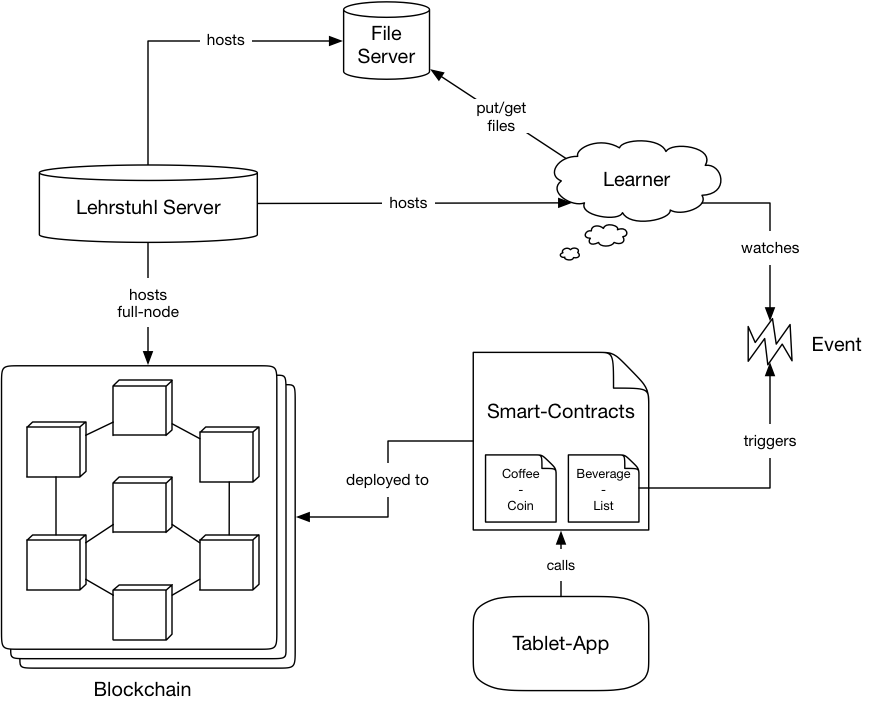
\includegraphics[width=.99\columnwidth]{./Abbildungen/Kapitel_03/system_architecture.png}
	\caption{Systemarchitektur}
	\label{img:abb1}
\end{figure}
\FloatBarrier

\nlparagraph{Lehrstuhl Server}
Der Lehrstuhlserver ist dafür zuständig einen Großteil der Anwendungen zu hosten bzw. zu starten.
Dies gilt sowohl für den HTTP-Fileserver als auch für die Learner-Anwendung, welche dessen Betriebssystem als Plattform nutzen.\\
Auch die Blockchain wird auf dem Server gestartet und verwendet diesen zudem als full-node, um Transaktionen zu minen.
Der Server ist im Grunde der Anwendungen, dessen primäre Funktionsweise darin besteht jenen eine Plattform zu bieten und mit Rechenleistung zu versorgen.

\nlparagraph{Learner}
Der sogenannte \quotes{Learner} ist eine in Golang implementierte Softwareanwendung, dessen Hauptaufgabe darin besteht, das Kaffeetrinkverhalten der Nutzer zu erlernen - wovon auch die Namensgebung der Anwendung stammt.
Um dies zu erreichen, wurde die Anwendung in Submodule unterteilt, welche einen dedizierten Aufgabenbereich abdecken und diesen eigenständig bearbeiten.
Auch wenn jene für sich autark agieren können, kann das Trinkverhalten letztendlich erst in der gegenseitigen Wechselwirkung jener erlernt werden. \\
Die Submodule lauten wie folgt:
\begin{itemize}
	\item Q-Learning
	\item Worker
	\item Watcher
	\item (Smart Contract Deployment Skript)
\end{itemize}

Das \textbf{Q-Learning} ist, wie der Name bereits impliziert, für das eigentliche Erlernen des Trinkverhaltens zuständig. Es ist im Grunde die Implementierung des Q-Learning Algorithmus, sowie die damit einhergehende Zustandsraummodiellerung, welches aber unter ref{subsec:ql} genauer erläutert wird.
\\\\
Der \textbf{Worker} ist einerseits für die Userverwaltung und andererseits für die, in einem festgelegten Intervall, Ausführung des Q-Learning Algorithmus, zuständig. (vgl. Kap. \ref{subsec:learning})
\\\\
Der \textbf{Watcher} beobachtet Events, die vom Smart-Contract \quotes{Beveragelist} ausgelöst wurden. Die Daten, welches das Event beinhaltet, werden daraufhin verwendet um den Q-Learning Algorithmus zu befüllen und aufgrund diesen das Trinkverhalten zu erlernen.
\\\\
Das \textbf{Smart Contract Deployment Skript}, ist in der Form zwar nicht in der Systemarchitektur vorhanden, da es aber auch ein Submodul des Learners und für das gesamte Konstrukt dahingehend essentiell ist, da es die Smart Contracts auf der Blockchain installiert und im Zuge dessen erst die Verbindung zwischen Blockchain und Learner ermöglicht, wird es in dieser Auflistung trotzdem aufgeführt.

\nlparagraph{Fileserver}
Der Fileserver ist eine Go-Anwendung, welche eine rudimentäre REST \cite{REST:Wiki} Api \cite{API:Wiki} zur Verfügung stellt.
Von den sogenannten CRUD \cite{CRUD:Wiki} Operationen, welche als grundlegend für alle persistenten Datenspeicher angesehen werden können, implementiert dieser nur das \quotes{GET} und das \quotes{PUT}. Sowohl die \quotes{PATCH} als auch die \quotes{DELETE} Operation bieten keinen Mehrwert für die Gesamtarchitektur bzw. den Workflow und sind in Anbetracht dessen nicht implementiert.\\
Das bedeutet die Hauptaufgabe des Fileservers besteht darin, Dateien zu empfangen und zu speichern (PUT) und diese auf Anfrage (GET) an einen Antragsteller wieder zu versenden.\\
Außerdem bietet die Anwendung zusätzlich zur Api einen UDP-Broadcast, welcher v.a. beim Testing und beim Setup eine große Erleichterung darstellt. Dieser Broadcast versendet in seinen Nachrichten lediglich die IP-Adresse des Lehrstuhl-Servers und somit auch seine eigene und die der Blockchain.
Da die IP-Adresse und der Port des Broadcasts stets gleich bleiben, sich aber die Host-IP der Blockchain und des Fileservers je nach Deployment theoretisch ändern können - was in der Entwicklungsphase sehr oft der Fall war. Müssen sich sowohl der Learner als auch die Tablet-App lediglich auf den Broadcast \quotes{subscriben} und können dadurch die IP der Blockchain und des Fileservers erfahren. Durch diese dynamische Zuweisung der IP-Adresse, müssen keine Updates beim Learner und der App durchgeführt werden, sollte die Blockchain und der Fileserver auf einem anderen Host deployed werden. \\
Aufgrund der Tatsache, dass sich die IP-Adresse des Lehrstuhl-Servers während der Studie nicht ändert, ist der UDP-Broadcast auch nicht in der Abbildung \ref{img:abb1} der Systemarchitektur berücksichtigt worden. Der Anwendungsbereich ist trotz alledem im Bereich der Testphase und auch für die künftige Projekte,bei denen das System Verwendung findet, definitiv vorhanden.

\clearpage
\nlparagraph{Blockchain}
Die Blockchain ist eine private, eigens für die Studie erstellte Ethereum-Blockchain, dessen \quotes{Genesis-Block} aus dem JSON-File (vgl. Abbildung \ref{img:abb3}) generiert wird. Die Erläuterungen zu den jeweiligen Key-Value-Pairs sind unter Kap. \ref{subsec:genesis} zu finden.
Das Generieren und das Starten der Blockchain erfolgt auf dem Lehrstuhlserver.
Dabei hostet der Server zudem eine sogenannte \quotes{full-node} (auch \quotes{miner} genannt) der Blockchain, welche dafür zuständig ist Transaktionen zu berechnen und zu bestätigen.
Aus Ressourcengründen ist dieser \quotes{miner} der einzige im Gesamtsystem, was aus theoretischer Sicht einen \quotes{Single Point of Failure} \cite{SPOF:Wiki} als Nachteil mit sich zieht. Das bedeutet sollte diese \quotes{full-node} ausfallen, würden keine Transaktionen mehr bestätigt werden. Da es weder während der Entwicklungsphase noch während der Studie zu einem einzigen Ausfall kam, ist dieser Nachteil als sehr klein einzuschätzen, weswegen auch keine weitere \quotes{full-node} zum System hinzugefügt wurde. Der große Vorteil besteht allerdings darin, dass Transaktionen sehr schnell bestätigt werden, da es keine weiteren \quotes{node's} gibt, die um die Berechnung eines Block's konkurrieren. Was vor allem aus Sicht der User-Experience \cite{UE:Wiki} einen großen Mehrwert darstellt, da dieser in wenigen Sekunden erfährt, ob seine Transaktion erfolgreich durchgeführt wurde. Dies kann bei anderen Blockchains wie z.B. Bitcoin bis zu 10 Minuten dauern \cite{MINING:kryptopedia}, was im Kontext der Systemarchitektur nicht tragbar wäre.\\\\
Um letztendlich mit der Blockchain kommunizieren und dessen Potential in voller Gänze ausschöpfen zu können, werden auf diese sogenannte Smart-Contracts \cite{SC:EconomyOutlook} deployed. Im Rahmen der Systemarchitektur sind es zwei dedizierte Smart-Contracts (\textit{Coffe-Coin}, \textit{Beverage-List}), welche komplett unabhängig voneinander agieren.

\clearpage
\nlparagraph{Smart Contracts}
Die beiden Smart Contracts welche auf die Blockchain deployed werden, werden mit \textit{Coffe-Coin} und \textit{Beverage-List} betitelt.
Diese decken zwei völlig unterschiedliche Aufgabenbereiche ab, weswegen sie keinen Einfluss aufeinander haben und deswegen unabhängig voneinander operieren.
So löst nur der \textit{Beverage-List Contract} ein Event aus, sobald eine bestimmte Funktion dessen aufgerufen wird. \\
Die Ausführung (\textit{call}) beider erfolgt jedoch stets von Seiten der \textit{Tablet-App}. Diese ist auch die einzige Instanz, welche in Form von Transaktionen mit der Blockchain interagiert.

\nlparagraph{Tablet-App}
Die \textit{Tablet-App} ist eine mit React-Native \cite{RN:ReactNative} erstellte Crossplattform App \cite{CP:Wiki}, welche auf einem Android Tablet installiert ist. Die Hauptaufgabe der App ist es Funktionen der beiden Smart Contracts aufzurufen, in dem es die benötigten Daten an den Smart Contract übergibt, um schlussendlich Transaktionen auszulösen.\\
Damit eine Kommunikation mit einem Smart Contract überhaupt zustande kommt, schickt die App einen Request an den Fileserver, welcher mit den angefragten Smart Contract Daten in Form einer Datei antwortet.
\nlparagraph{Event}
Das Event beschreibt im Grunde die indirekte Kommunikation zwischen dem \textit{Learner} und der \textit{Tablet-App} mit dem Smart Contract \textit{Beverage-List} als Mittelsmann. So wird jenes im Zuge eines Funktionsaufrufs des Smart Contracts von Seiten der App ausgelöst und vom \textit{Learner} detektiert und der Inhalt zum Erlernen des Kaffeetrinkverhaltens verwendet.
\clearpage

\subsection{Workflow}
\label{subsec:workflow}
Die unter Kap. \ref{subsec:architecture} beschriebene Architektur wird im folgenden unter dem Gesichtspunkt des Workflows, also dem Zusammenspiel der einzelnen Komponenten und dem Gesamtablauf, näher betrachtet. Dabei beschreibt der Gesamtablauf die einzelnen Schritte startend beim Setup der Komponenten hin zum eigentlichen Durchlauf der einzelnen Softwareanwendungen, was letztlich im Erlernen des Kaffeetrinkverhaltens resultiert. Im Zuge dessen werden auch einzelne Algorithmen der Instanzen und Kommandos kurz erläutert, um ein besseres Verständnis für die Funktionsweise der Anwendungen zu bekommen. \\\\
Der Workflow lässt sich in zwei Phasen unterteilen. In der ersten werden die einzelnen Komponenten konfiguriert und gestartet und die zweite beschreibt den eigentlichen Ablauf und das Zusammenwirken der Instanzen.

\paragraph{Setup}
\begin{legal}
	\item {Blockchain}
	\begin{legal}
		\item erstellen \& konfigurieren
		\item starten
	\end{legal}
			      	       	                            
	\item Fileserver
	\begin{legal}
		\item REST Api starten
		\item UDP Broadcast starten
	\end{legal}
			      	       	                            
	\item Smart Contracts
	\begin{legal}
		\item deploy Beveragelist Smart Contract und sende JSON-File mit ABI und Adresse an Fileserver
		\item deploy CoffeeCoin Smart Contract und sende JSON-File mit ABI und Adresse an Fileserver
	\end{legal}
			      	       	                            
	\item Learner
	\begin{legal}
		\item Worker starten
		\item Watcher starten
	\end{legal}
			      	       	                            
	\item Tablet App
	\begin{legal}
		\item installieren
		\item starten
	\end{legal}
			      	       	                                
\end{legal}

Die Punkte 1. und 2. sowie 4. und 5. können auch parallel ausgeführt bzw. deren Reihenfolge vertauscht werden.\\\\
Im ersten Schritt muss die private Blockchain erstellt werden. Dabei müssen zuerst die benötigten Accounts generiert und daraufhin die Blockchain erzeugt werden. Sollte 1a) zu einem früheren Zeitpunkt bereits durchgeführt worden sein, kann dieser Punkt übersprungen und gleich mit 1b) begonnen werden.
Sobald 1a) einmal durchgeführt wurde, kann die Blockchain gestartet werden.
\\\\ Dies geschieht mit folgendem Befehl:\\

\newlength{\imageheight}
\settoheight{\imageheight}{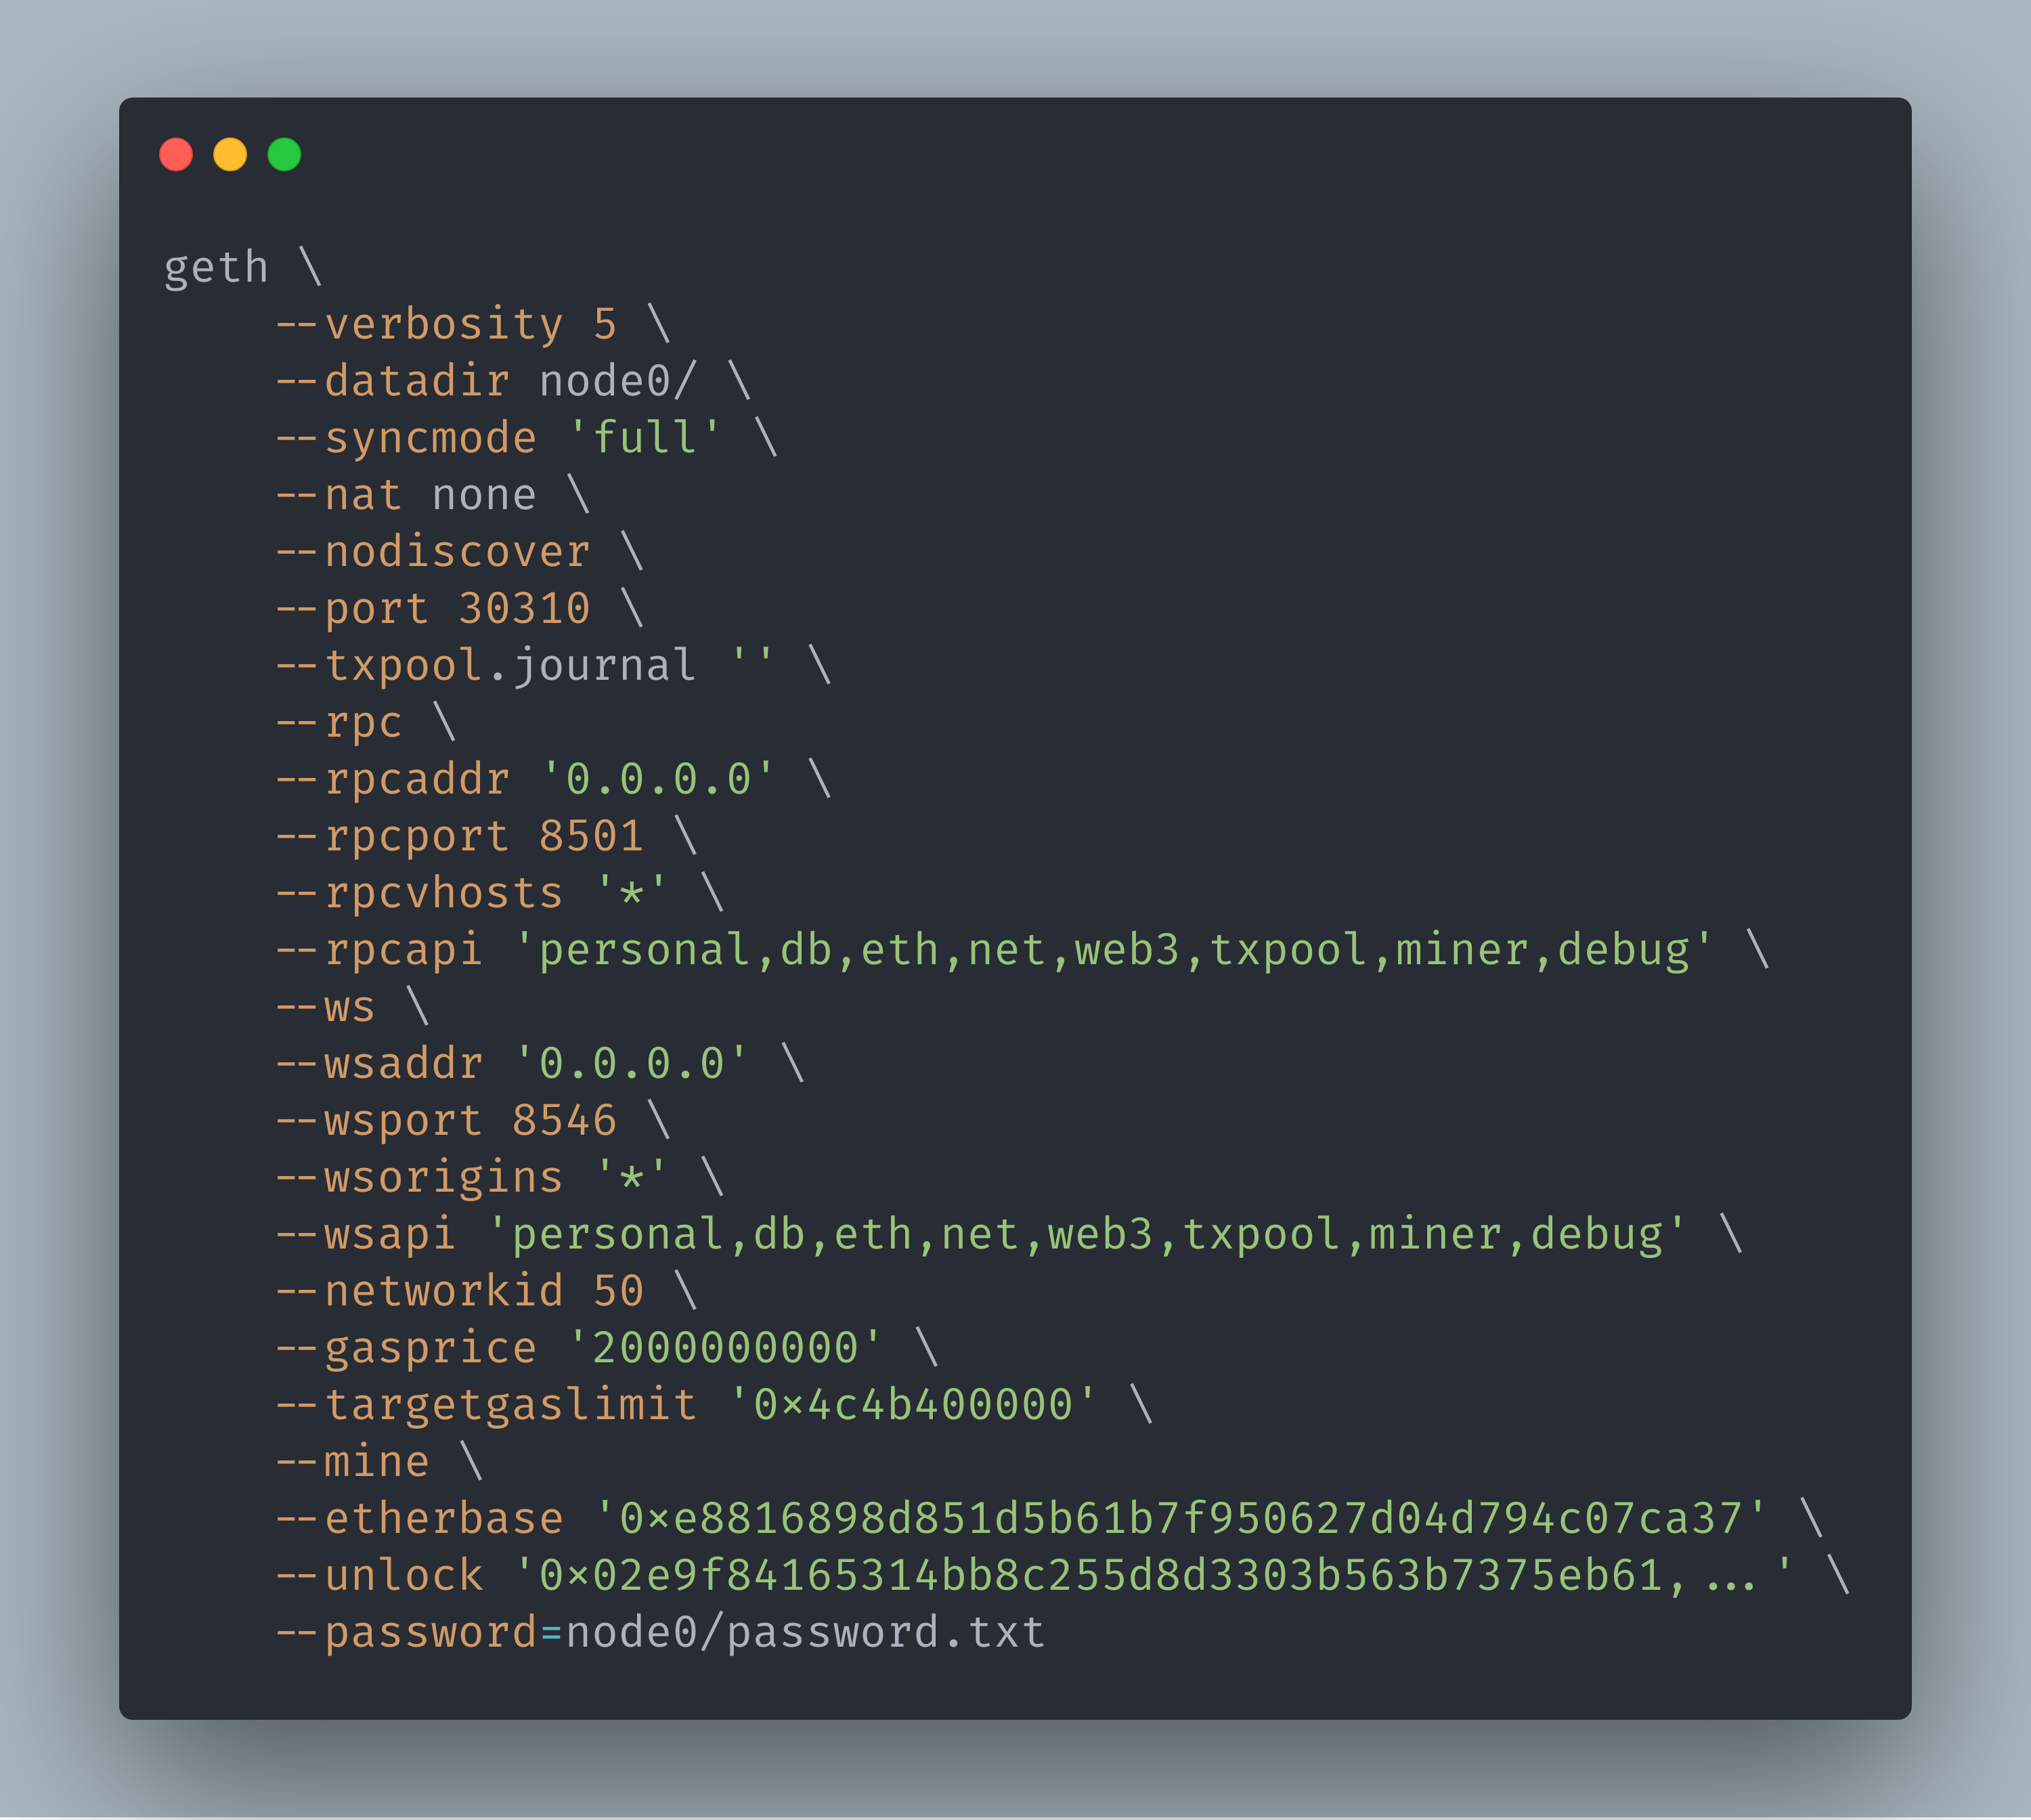
\includegraphics{./Abbildungen/Kapitel_03/geth.png}}
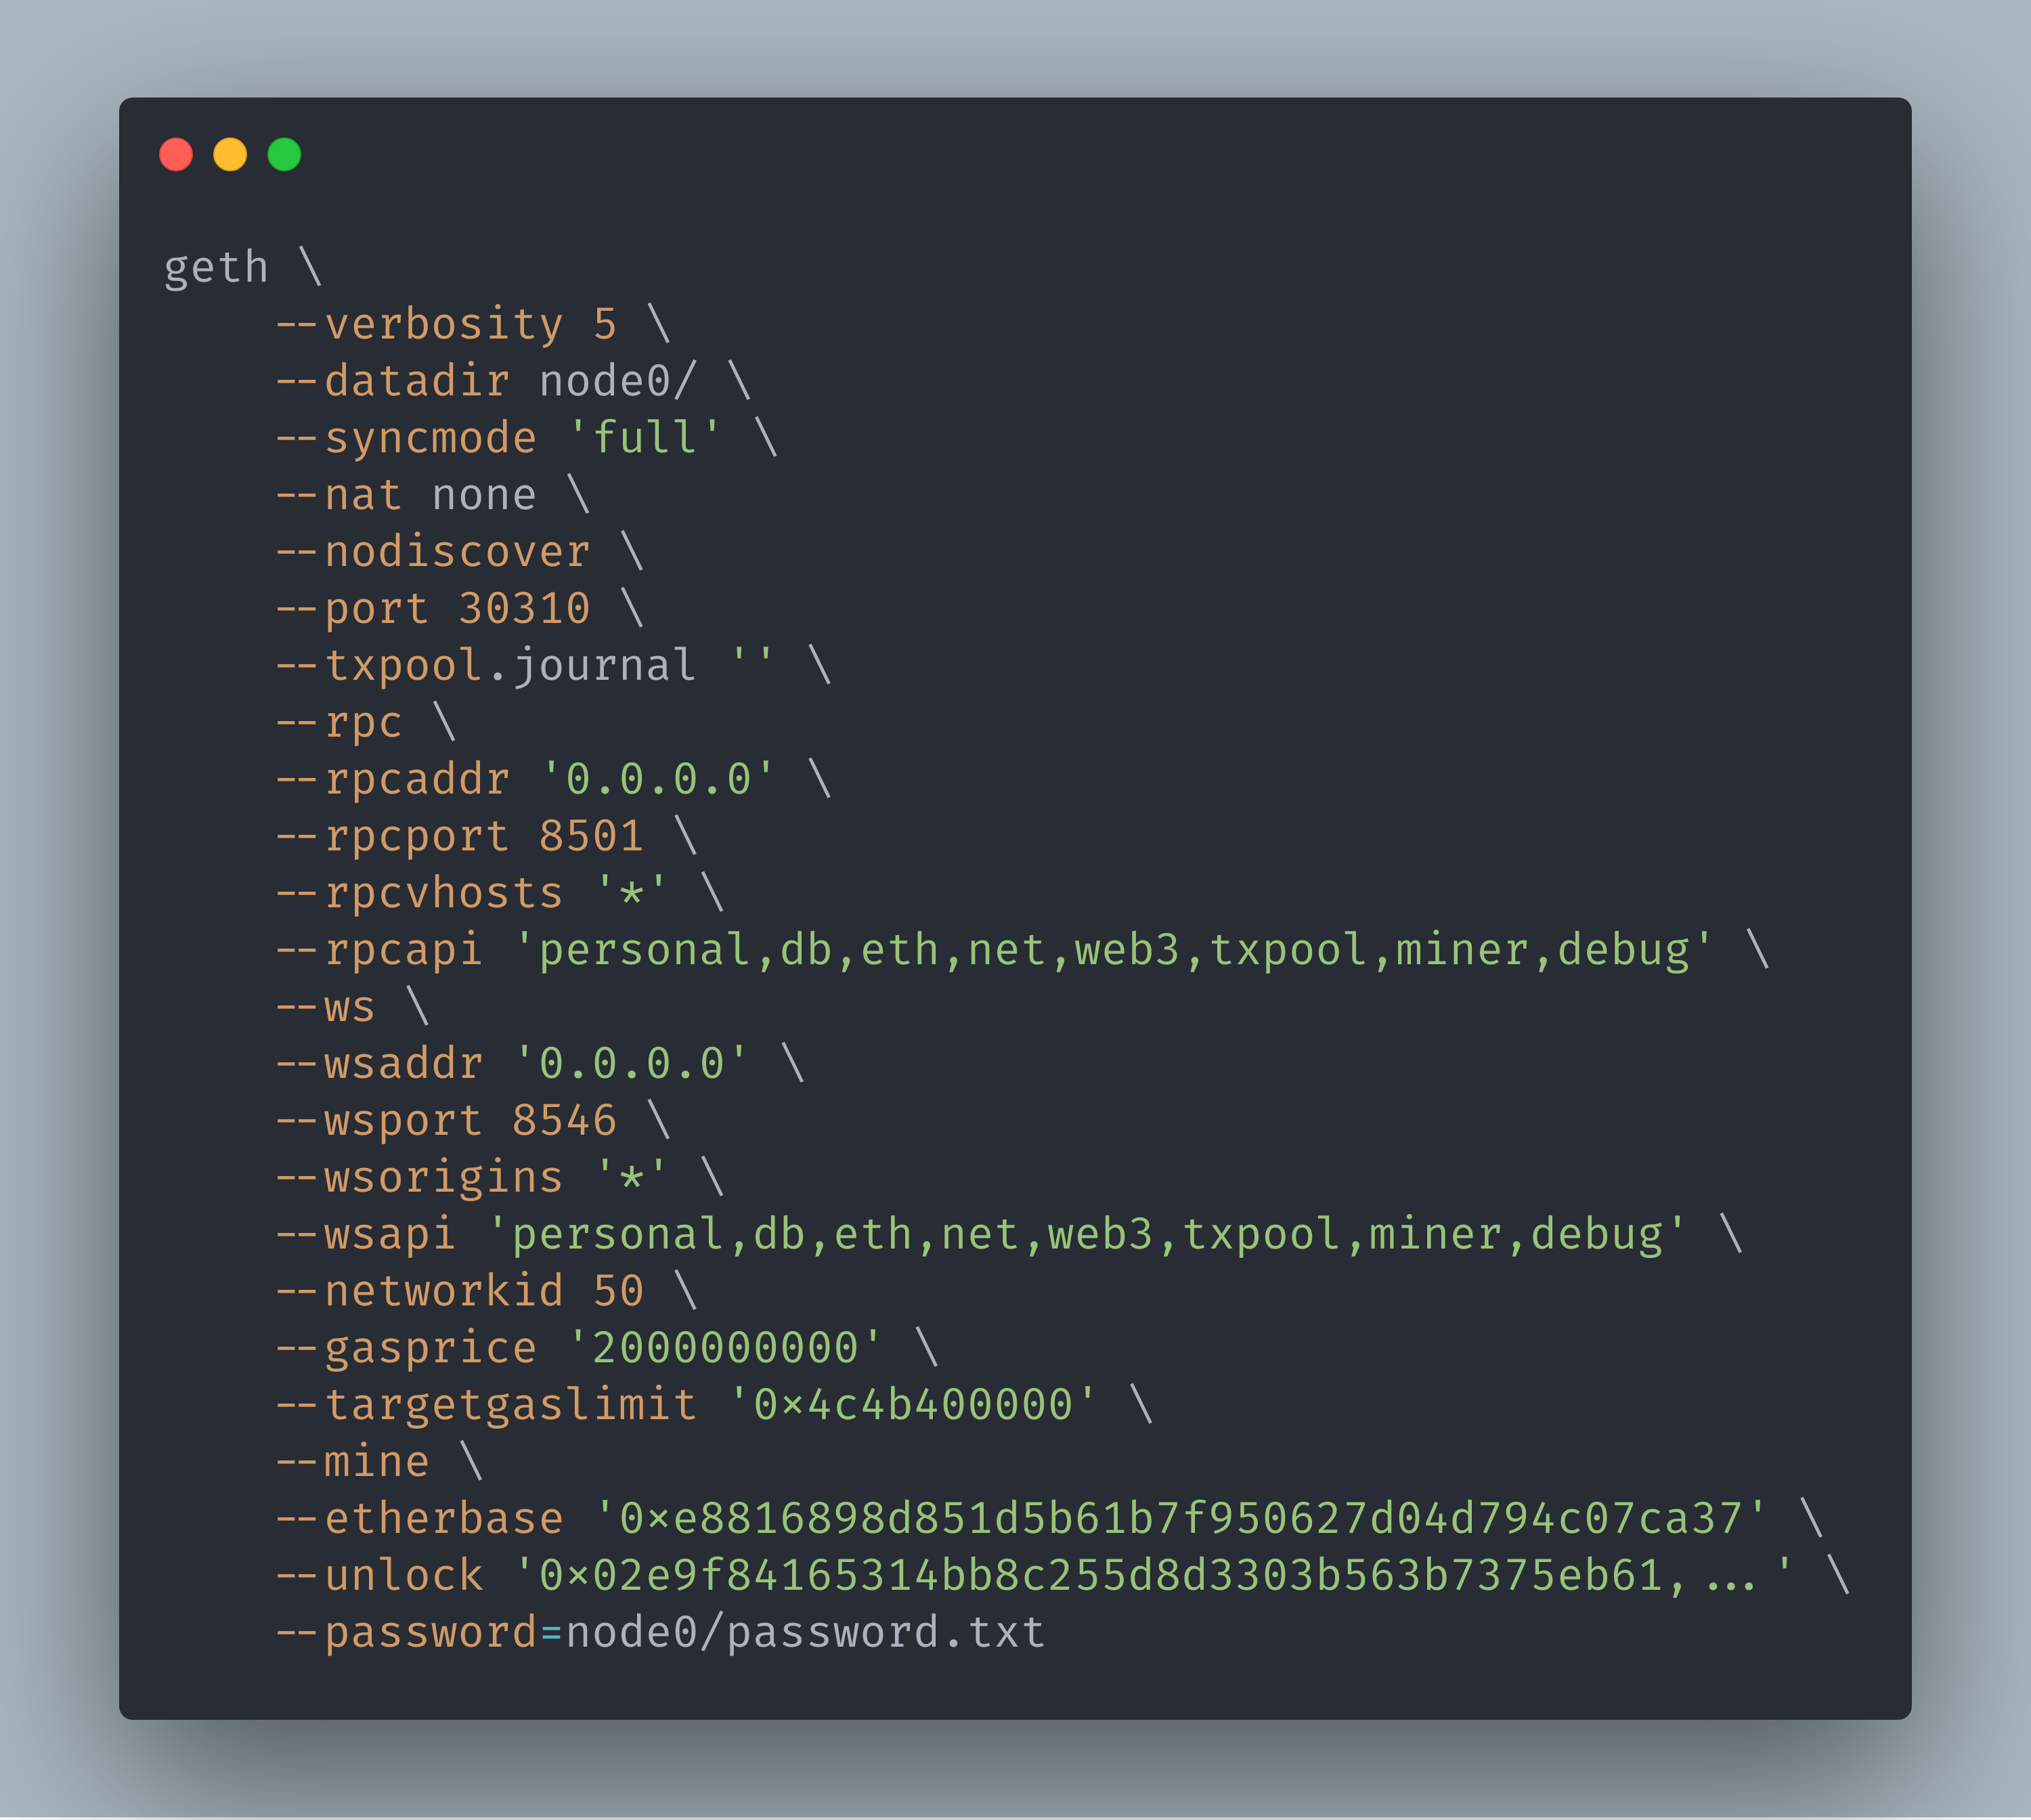
\includegraphics[trim=0 0.49\imageheight{} 0 0, clip, width=.9\columnwidth]{./Abbildungen/Kapitel_03/geth.png}

\clearpage

\begin{figure}[hbt!]
	\centering
	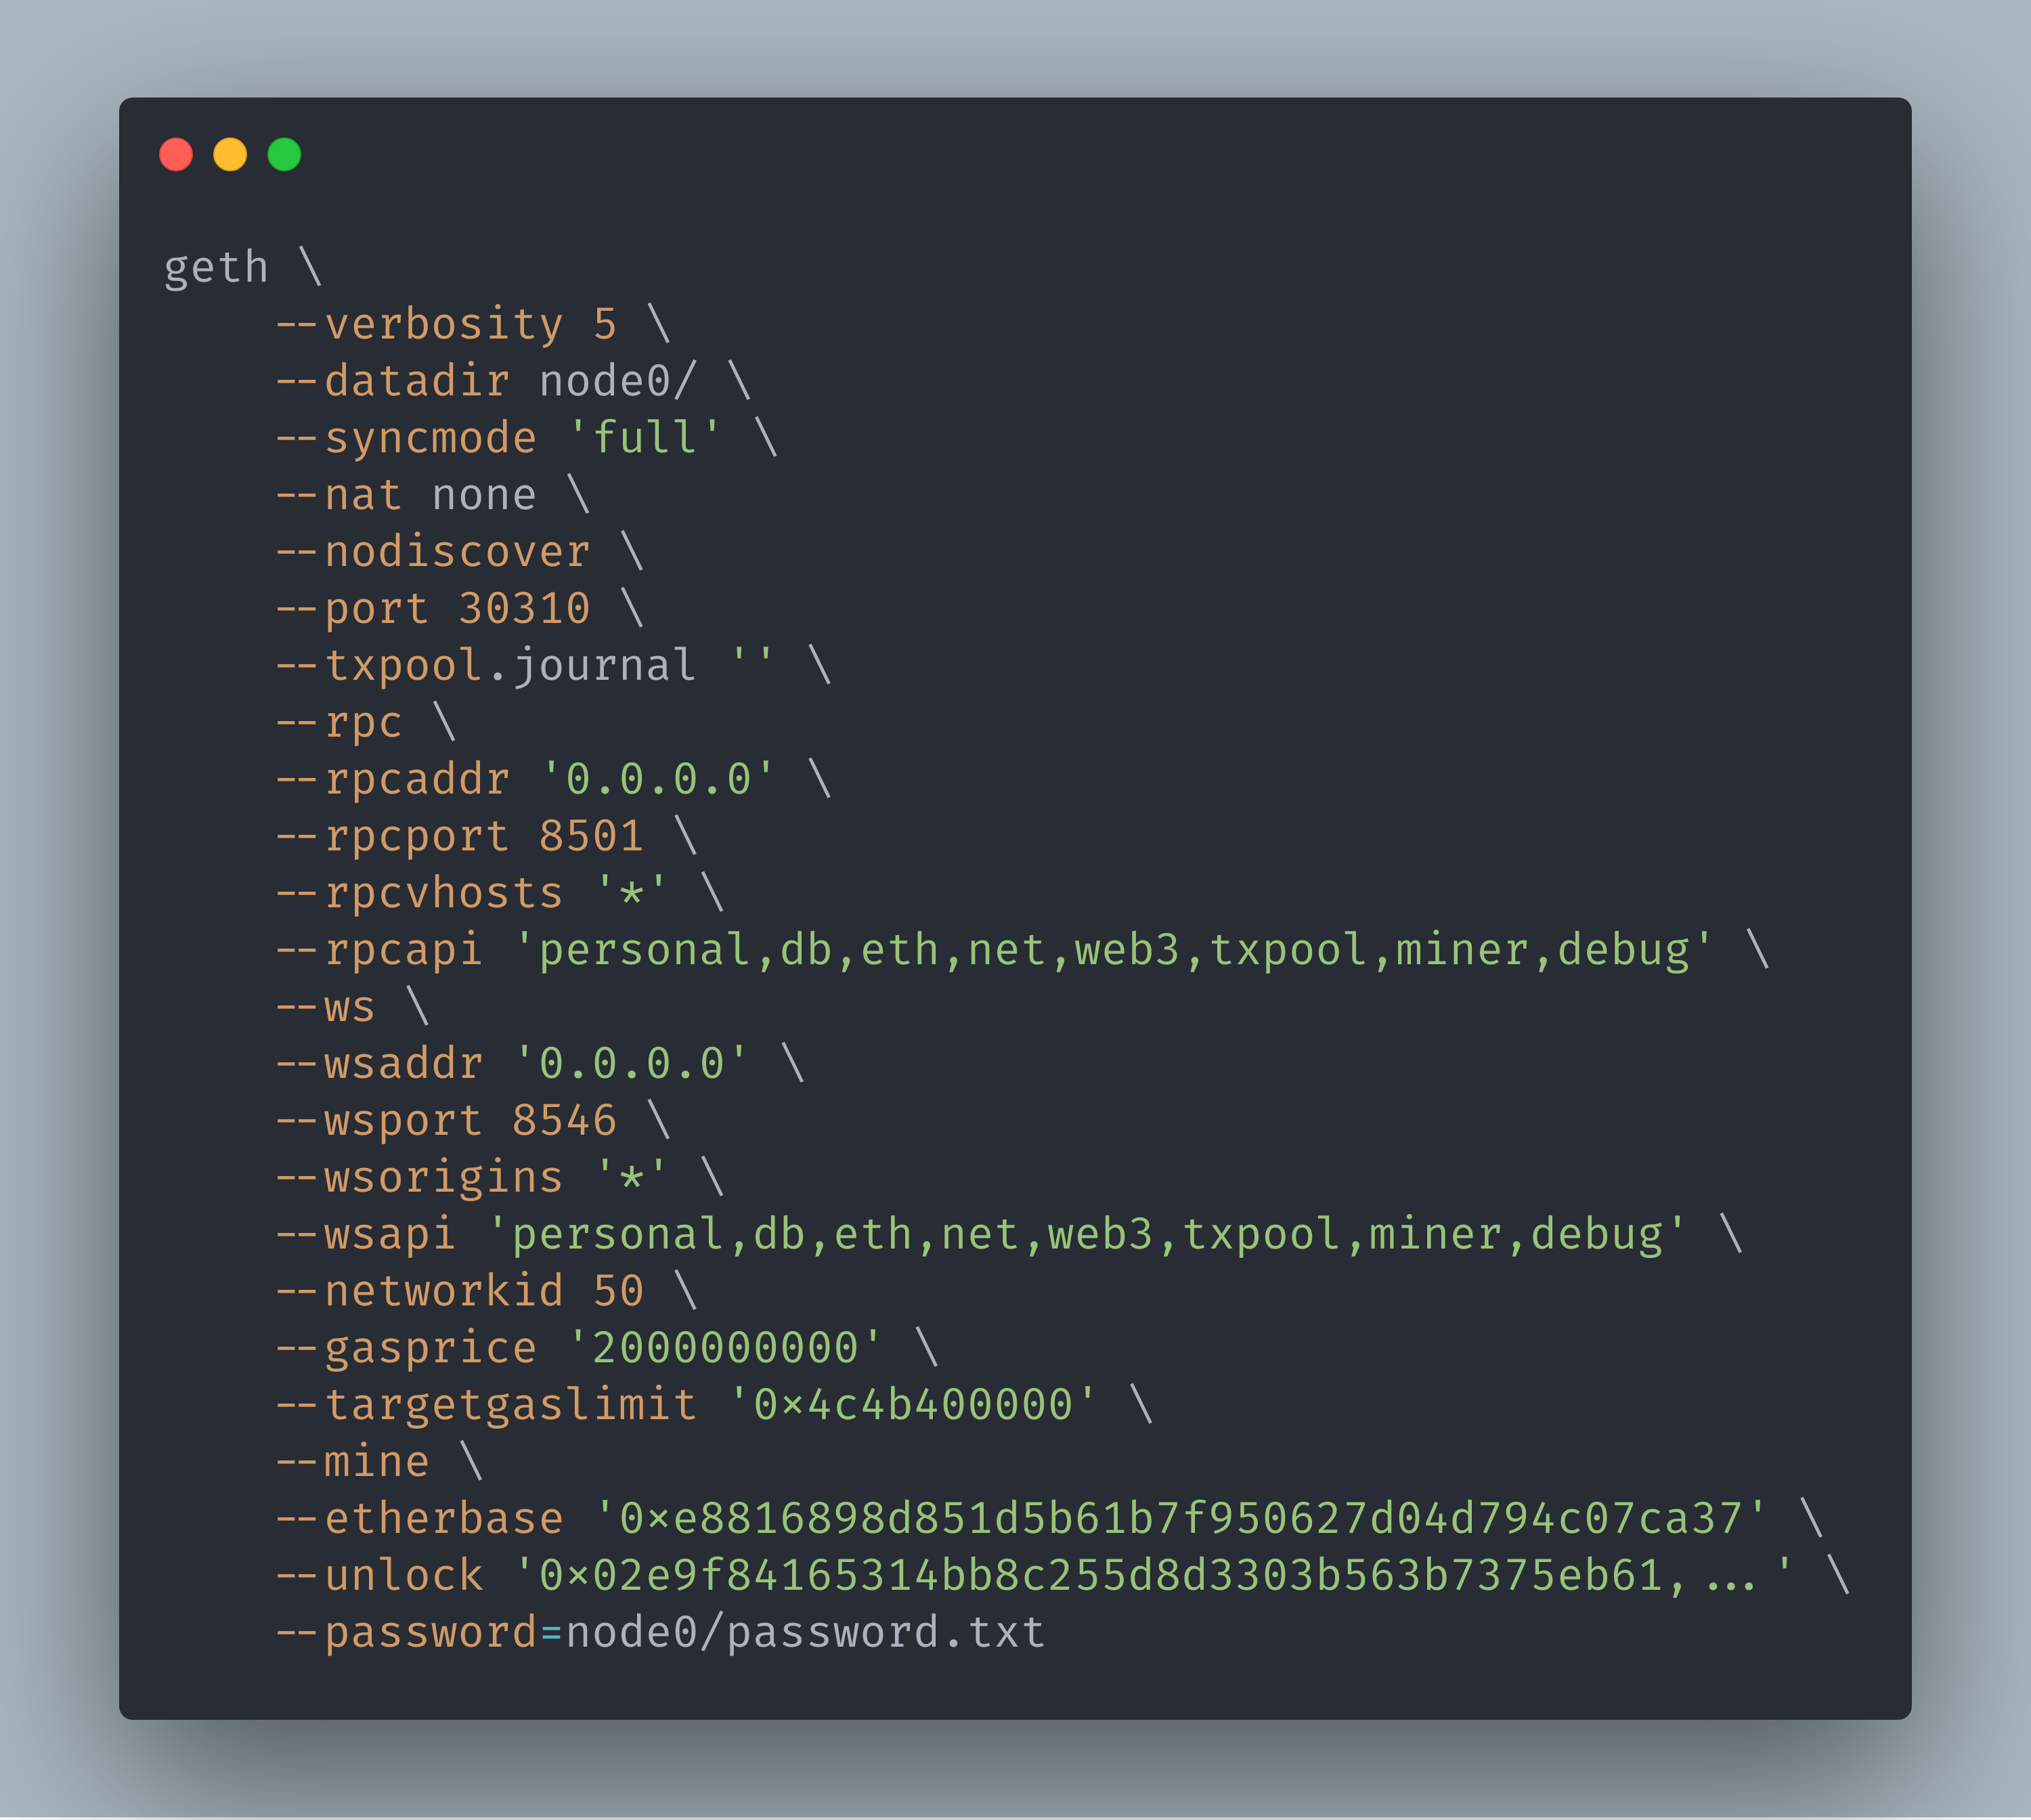
\includegraphics[trim=0 0 0 0.503\imageheight{}, clip, width=.9\columnwidth]{./Abbildungen/Kapitel_03/geth.png}
	\caption{geth Befehl zum starten der Blockchain}
	\label{img:geth}
\end{figure}

Dieser Befehl setzt zum einen weitere Konfigurationsparameter der Blockchain. So wird z.B. festgelegt unter welcher IP-Adresse und Port (\textit{-{}-rpcaddr}, \textit{-{}-rpcport}, \textit{-{}-wscaddr}, \textit{-{}-wsport}) die Blockchain erreichbar ist und welche Api-Befehle unter dieser Schnittstelle ausgeführt werden dürfen (\textit{-{}-rpcapi}, \textit{-{}-wsapi}). \\
Zum anderen wird aber zugleich auch eine sogenannte \textit{full node} gestartet (\textit{-{}-syncmode}), die durch das \quotes{Flag} \textit{-{}-mine} sofort zum \quotes{minen} beginnt.\\
Desweiteren werden alle Accounts entsperrt die unter (\textit{-{}-unlock}) gelistet sind und deren Passwörter in der angegebenen Textdatei bei (\textit{-{}-password}) hinterlegt sind. \\\\
Damit eine \textit{Node} Daten speichern kann, muss ein Verzeichnis angegeben werden (\textit{-{}-datadir}), in dem Dateien abgelegt werden können. Hier werden z.B. die Daten der Accounts oder auch die Textdatei mit den Passwörtern (\textit{-{}-password}) gespeichert.\\\\
Wurde die Blockchain in Betrieb genommen, wird im nächsten Schritt die REST Api und der UDP Broadcast des Fileservers gestartet. \\
Daraufhin ist es möglich die beiden Smart Contracts zu deployen. Dabei wird jeweils für 3a) und 3b) das identische Bash-Skript mit unterschiedlichen Eingabeparametern ausgeführt. Dieses Skript liest zuerst die Datei des angegebenen Smart Contracts ein und erzeugt daraufhin die Binaries und die ABI,
welche schlussendlich dazu verwendet werden ein Go Bindingsfile zu generieren.
Im Anschluss wird dann ein Go-Skript ausgeführt, welches auf Grundlage des Bindingsfiles den Smart Contract auf der Blockchain installiert und die zurückgelieferte Adresse und die bereits bekannte ABI ein JSON-File packt und an den Fileserver schickt.\\\\
Wurden die Smart-Contracts erfolgreich deployed, kann der Learner gestartet werden. Dieser \quotes{subscribed} sich im ersten Schritt auf den UDP Broadcast und extrahiert aus den Nachrichten die IP-Adresse der Blockchain und des Fileservers. Daraufhin werden sowohl der Worker als auch der Watcher in Form von \quotes{Goroutines} aktiviert. Der Worker iteriert über die Liste aller User und kontaktiert jeweils den Fileserver ob bereits gelernte Daten für diesen Usern vorhanden sind. Sollte das Fall sein, initialisiert er damit die Parameter des Q-Learning Algorithmus des Users.\\
Der Watcher schickt ebenfalls eine Anfrage an den Fileserver und bekommt als Antwort die Daten der Smart Contracts. Daraufhin kann er sich mit der Blockchain verbinden und sich auf die Events des Beveragelist Smart Contracts \quotes{subscriben}.\\\\
Abschließend wird die App auf dem Tablet installiert, sollte sich diese noch nicht auf dem Tablet befinden und daraufhin gestartet. Die Initialisierung erfolgt hierbei nach dem selben Prinzip wie beim Learner. Zuerst wird der UDP Broadcast nach der Server Adresse abgefragt, mit welcher anschließend der Request an den Fileserver geschickt wird, um die benötigten Smart Contract Daten zu bekommen. Welche im Anschluss dazu verwendet werden eine Verbindung zur Blockchain bzw. zu den Smart Contracts herzustellen.
\\\\
Erfolgte eine fehlerlose Abarbeitung dieser Schritte, kann zum eigentlichen Workflow übergegangen werden.
\clearpage
\paragraph{Workflow}
\begin{legal}
	\item {App}
	\begin{legal}
		\item User wählt Getränk aus
		\item \textit{call} CoffeeCoin
		\item \textit{call} Beveragelist
	\end{legal}
			      	       	                            
	\item Smart Contracts
	\begin{legal}
		\item Beveragelist \textit{triggers} Event
	\end{legal}
			      	       	                              
	\item Learner
	\begin{legal}
		\item Watcher:
		\begin{legal}
			\item detektiert Event
			\item extrahiert Daten aus Event
			\item befüllt Q-Learning Algorithmus mit den Event-Daten (evaluate \& predict)
		\end{legal}
		\item Worker (periodisch alle 3h)
		\begin{legal}
			\item \quotes{triggers} Q-Learning Algorithmus (evaluate \& predict)
			\item sendet gelernte Daten (vgl. Abbildung \ref{img:abb2}) an Fileserver
		\end{legal}
	\end{legal}
\end{legal}

Diese Auflistung beschreibt einen synchronen, erfolgreichen Durchlauf der Systemarchitektur - die Asynchronität des Workers 3b) außer Acht gelassen. Alternative Abläufe sowie Zustände die aus Fehlern resultieren, werden bei den einzelnen Komponenten nochmals genauer betrachtet.\\\\
Der Workflow wird durch den User gestartet indem dieser auf Tablet ein Getränk auswählt und eine Transaktion auslöst. Zuerst wird dabei der CoffeeCoin Contract aufgerufen und das ausgewählte Getränk bezahlt. Nachdem diese Transaktion erfolgreich bestätigt wurde, wird als nächstes der Beveragelist Contract ausgeführt. Die dabei aufgerufene Funktion des Smart Contracts verwendet die übergebenen Daten (Zeit, Getränk, Wochentag, Eth-Adresse) und löst damit ein Event aus. \\
Dieses Event wird vom Watcher detektiert und die Daten (Zeit, Getränk, Wochentag, Eth-Adresse) daraus extrahiert. Daraufhin wird die \textit{Learn-Methode} des Q-Learning Algorithmus aufgerufen, bei der zuerst die vorherige \quotes{Prediction} evaluiert und basierend auf dem aktuellen Zustand eine neue \quotes{Prediction} gemacht wird. \\
Zu diesem synchronen Durchlauf führt der Worker am Ende jedes Timeslots (alle 3h) die \textit{Learn-Methode} für jeden bekannten User aus. Das heißt es werden wie auch beim Watcher die \quotes{Predictions} des vorangegangen Timeslots evaluiert, neue \quotes{Predictions} für den kommenden Timeslot erstellt und die gelernten Daten als Datei an den Fileserver gesendet.

\clearpage

\subsection{Entwicklungsprozess}
Abschließend wird der Prozess der Entwicklung geschildert, aus welchem schließlich die finale Version der Systemarchitektur resultierte. \\
Der Entwicklungsprozess beinhaltete mehrere Iterationen der einzelnen Komponenten bis hin zum derzeitigen Stand. Das Konzept sah primär die Entwicklung von drei dedizierten Software Anwendungen vor, welche aber im Zuge der Iterationen nochmal in kleinere Module aufgeteilt und ausgelagert wurden. Zudem wurden, um den Workflow und das Testen während der Entwicklungsphase zu erleichtern, Anwendungen entwickelt, welche während der Konzeption in der Art nicht vorgesehen waren, aber partiell Bestandteil der Systemarchitektur wurden. \\
So wurde mit zwei separaten Repos gestartet, einerseits für den Learning-Part, welcher anfänglich auch die Smart Contracts umfasste, und andererseits eines für die Tablet-App, welches bereits vor der eigentlichen Konzeption erstellt wurde, um in erster Linie bestehende Crossplattform Frameworks, auf Basis der Kompatibilität und Funktionstüchtigkeit mit Libraries, welche die Kommunikation mit der Blockchain ermöglichen, zu evaluieren. \\
Die Wahl fiel letztendlich auf React-Native, welches zwar nur bis zu einer bestimmten Versionsnummer der Web3.js Library von Ethereum vollends kompatibel ist und nur mit einem kleinen Workaround zum Laufen gebracht werden konnte.
Jedoch im Vergleich zu anderen Frameworks (z.B. Nativescript) die beste Development-Experience (geringe Lernkurve, gute Dokumentation, CLI) bot und v.a. hinsichtlich der Requirements alle Aufgaben komplett erfüllen konnte, welche die anderen Frameworks in dieser Gänze nicht replizieren konnten. \\
Nachdem die erste rudimentäre Version der Tablet-App, welche lediglich eine funktionierende Kommunikation (read/write) mit einem bereits bestehenden Smart-Contract auf einer lokal gehosteten Blockchain bestätigte, erstellt wurde, kam im nächsten Schritt der Learning-Part zum Zuge. \\\\
In Anbetracht der kompletten Implementierung des Ethereum Protokolls in Golang und der Schwierigkeiten mit der Javascript Library Web3.js, v.a. im Bezug auf das deployen der Smart-Contracts, aus einem vorangegangen Projekt, fiel die ´Wahl für diese Instanz auf Golang. \\
Zuerst wurde der Q-Learning Algorithmus, welcher für das Erlernen des Kaffee Trinkverhalten zuständig ist, implementiert. Die Problematik bestand zum einen darin mit einer neuen Programmiersprache vertraut zu werden und zum anderen den Workflow hinsichtlich der Problemstellung und des daraus resultierenden Zustandsraums vollends abzubilden. Die Umsetzung des Algorithmus in der Programmiersprache ging relativ einfach von der Hand, was jedoch Probleme bereitete war die Simulation des Workflows, um die Algorithmus Parameter zu justieren und dessen Tauglichkeit bezüglich das Erlernen des Nutzerverhaltens zu testen.\\\\
Im Anschluss wurde ein erster Smart-Contract erstellt und via dem “go-ethereum” package deployed, woraus das erste Smart-Contract Bindingsfile resultierte, welches für die Kommunikation mit dem Smart Contract vonnöten ist. Da mit jedem neuem Deployment eines Smart Contracts eine neue Smart Contract Adresse und eine neue ABI hervorgeht, welche wiederum beide im Source Code für die Kommunikation mit dem Smart Contract, über alle Instanzen hinweg, die mit einem Smart Contract interagieren wollen, hinterlegt sein müssen, wurde ein kleiner HTTP-Fileserver entwickelt, auf dem diese Informationen gespeichert und gelesen werden können. \\
Bei jedem neuen Deployment werden daraufhin die Smart-Contract Adresse und die generierte ABI in ein JSON-File gepackt und an den Server geschickt. So konnte während der Entwicklung enorm an Zeit gespart werden, da sich sowohl die Learning-Instanz als auch die App, die benötigten Daten vom Server holen und somit ein ständiges “Hardcodieren” dieser Daten vermieden werden konnte. \\
Aus diesem Grund findet der Fileserver auch Einzug in die finale Systemarchitektur, da er als persistente Datenquelle eine enorme Erleichterung nicht nur im Entwicklungsprozess, sondern auch im “Live-System” darstellt. \\
Zudem wird der Fileserver auch für die Verwaltung der Algorithmus-Daten verwendet. Dabei wird bei jedem Worker-Durchlauf (vgl. Kap. \ref{subsec:learning}) für jeden Nutzer ein JSON-File erzeugt, welches folgende Key-Value-Pairs beinhaltet (vgl. Kap. Abbildung \ref{img:abb2}):
\begin{itemize}
	\item qt: die aktuelle Q-Tabelle des Users
	\item ep: der aktuelle Epsilon-Wert
	\item negs: Anzahl der falschen Predictions in der aktuellen Woche
	\item Wk\_negs: Array von negs über alle Wochen hinweg
\end{itemize}


\begin{figure}[th!]
	\centering
	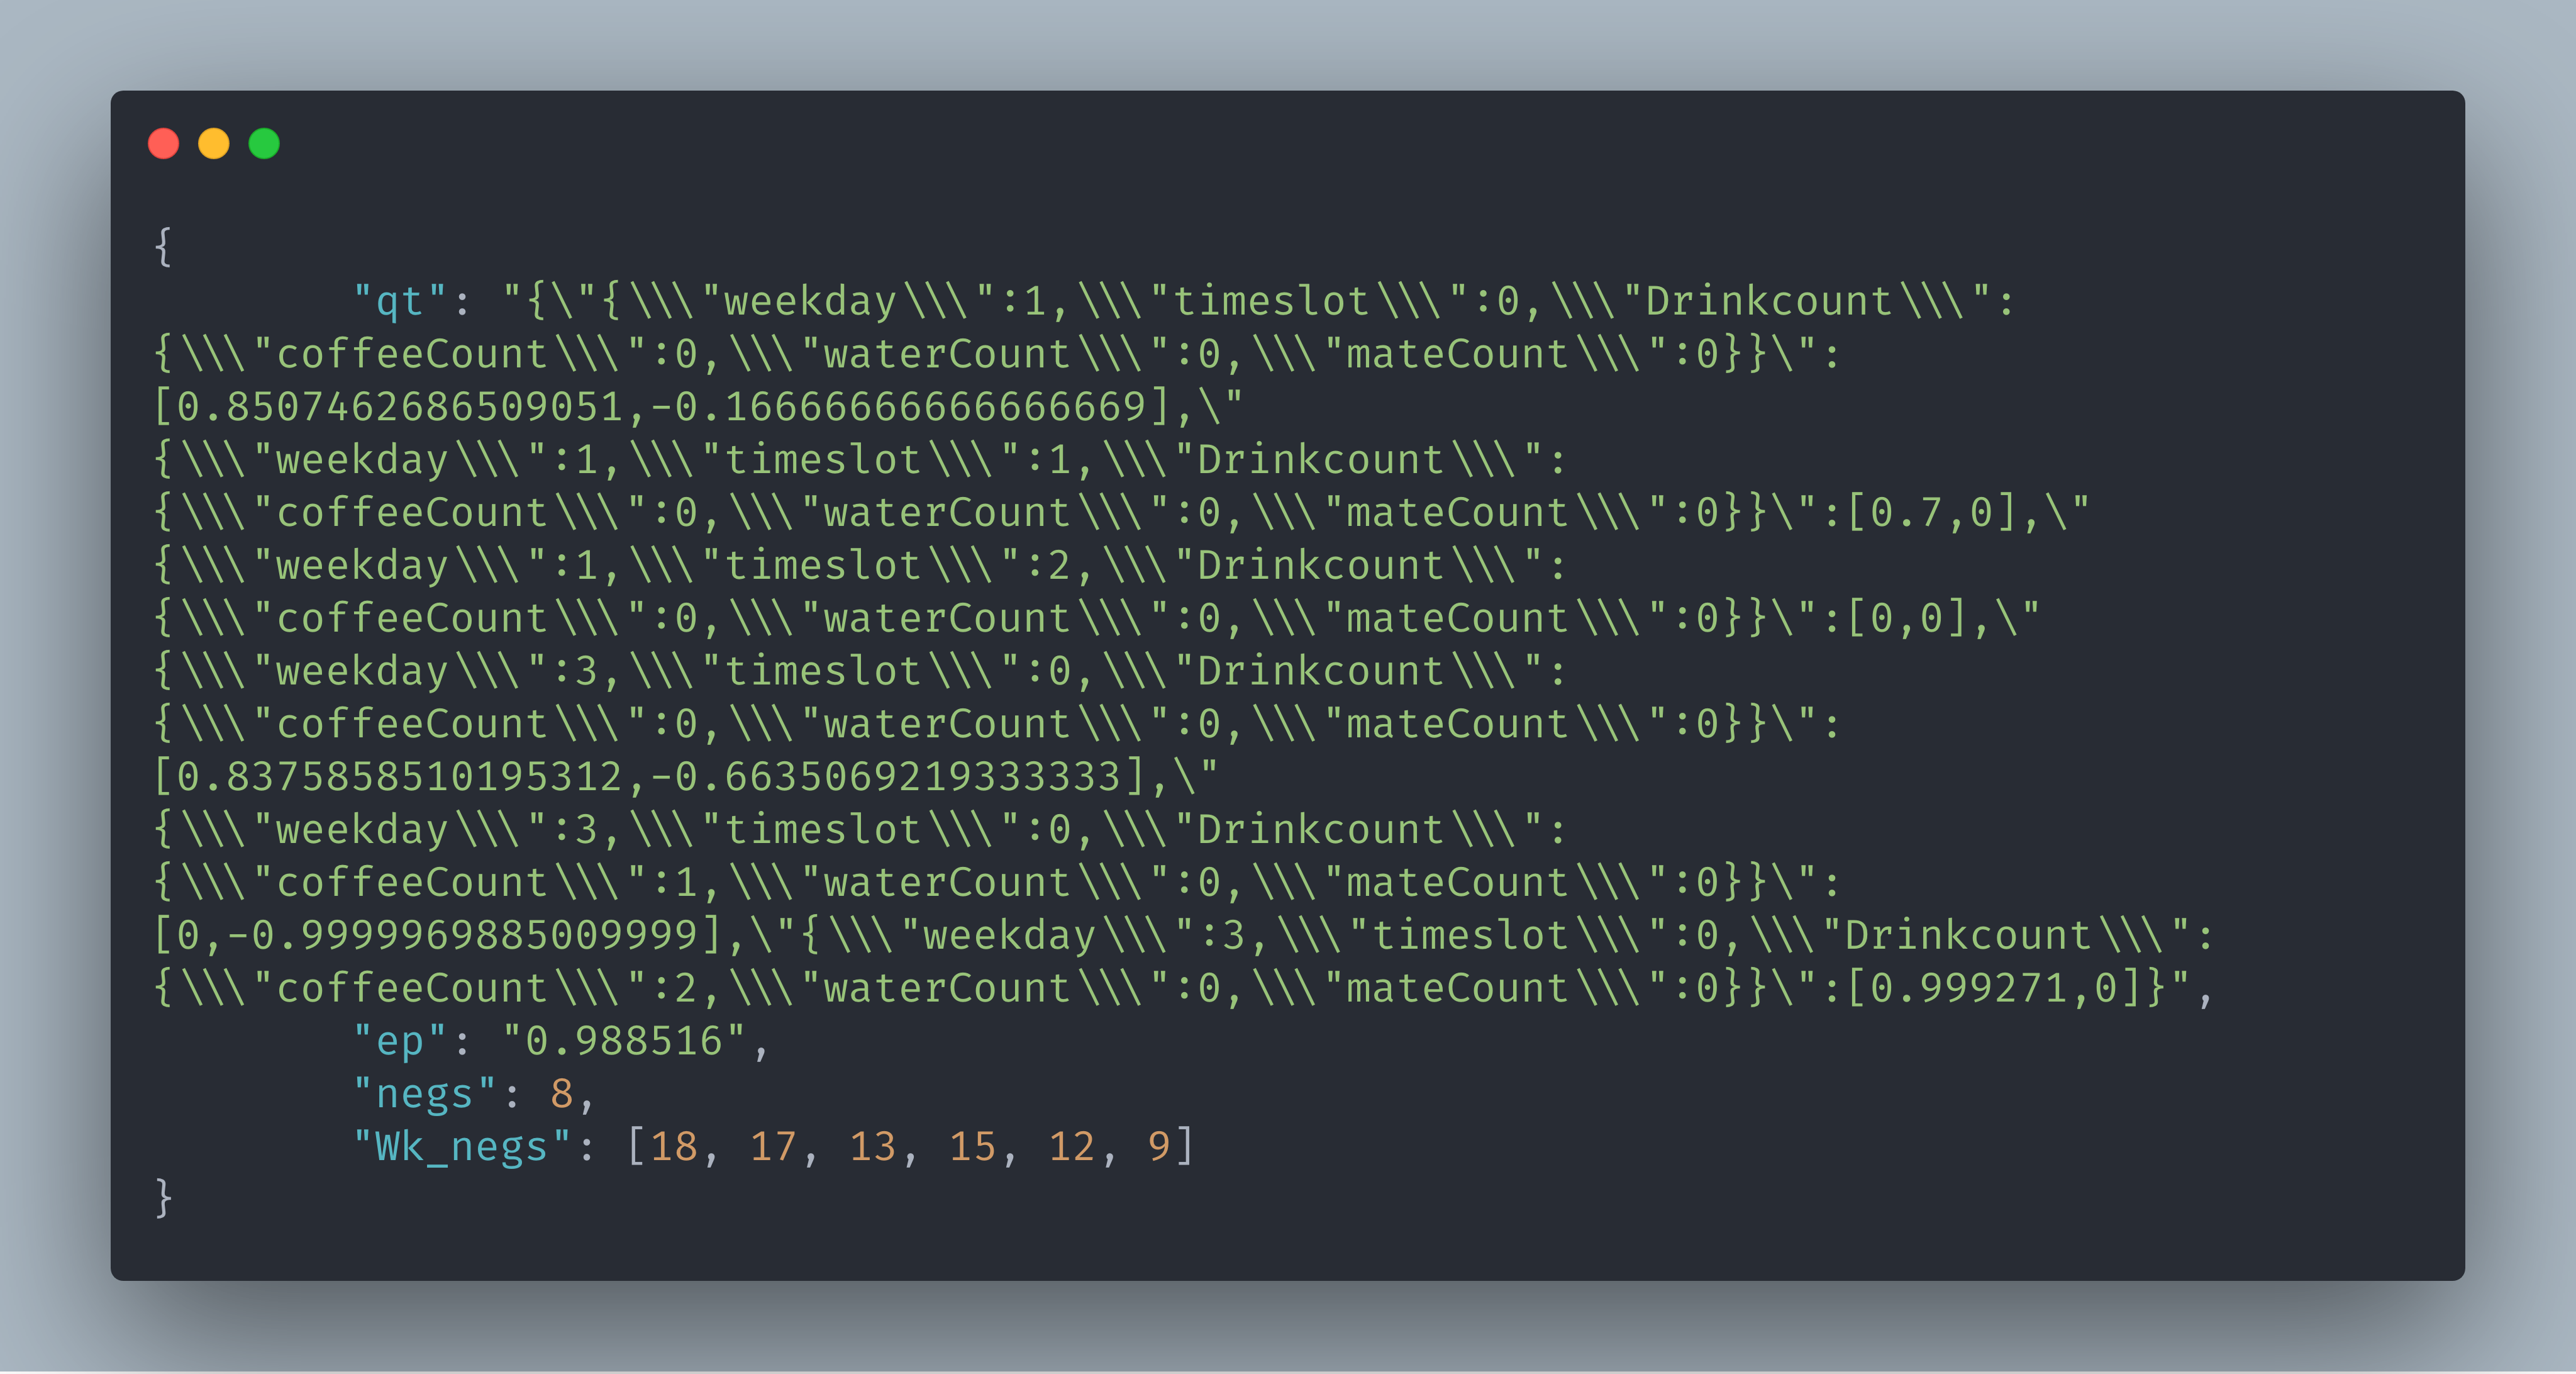
\includegraphics[width=.9\columnwidth]{./Abbildungen/Kapitel_03/usr_json.png}
	\caption{
		0x6ecbe1db9ef729cbe972c83fb886247691fb6beb-ql.json\\
		Der Name des JSON-Files setzt sich aus der Ethereum-Adresse des Users und der Abkürzung "ql", welches für Q-Learning steht, zusammenhängen.
	}
	\label{img:abb2}
\end{figure}

Der Vorteil liegt in der Möglichkeit den Learner jederzeit upzudaten ohne die gelernten Daten zu verlieren. Denn wird der Learner gestartet, holt sich dieser zuerst die Files vom Server, liest die Daten aus und initialisiert schon im Vorab die Q-Tabelle und das Epsilon eines jeden Users. \\
Sollte der Learner aus unbestimmten Gründen abstürzen, ist durch den eben beschriebenen Algorithmus die Erhaltung des Lernfortschrittes trotzdem sichergestellt.\\\\
Als letztes Modul wurde ein kleiner Node-Server entwickelt, dessen Aufgaben darin bestand die Smart-Contracts zu testen und als primitiver Ersatz für die App zu fungieren. Hierbei erzeugte er in einem festgelegten Intervall (7sek) Events mit einem zufällig generierten Daten (User \& Getränk) auf der Blockchain, um letztendlich die Event-Erkennung (“Watcher”) des “Learners” zu testen. Dabei wurde sowohl für den \quotes{Beverage-List Contract} als auch für den \quotes{CoffeeCoin-Contract} eine entsprechende Implementierung angefertigt.
\\In diesen Fällen wurde das Q-Learning-Submodul des Learners gar nicht erst gestartet, da lediglich die Funktionsweise des Watchers getestet werden sollte.\\
Besonders hier zeigte sich die Nützlichkeit des Fileservers, da gerade in der Entwicklungsphase die Smart-Contracts noch häufigen Änderungen unterlagen und dahingehend sehr oft neu deployed werden mussten, was ohne den Fileserver dazu geführt hätte die Smart Contract Daten bei jeder Iteration neu im Sourcecode zu hinterlegen.\\
Nach einer längeren Testphase, in der eine einwandfreie Kommunikation mit den beiden Smart Contracts attestiert werden konnte, wurde mit der eigentlichen Entwicklung der App begonnen, für jene auch Teile der Node-Server Implementierung übernommen werden konnten.\\
Schwierigkeiten traten dabei erst in der Testphase auf, in der festgestellt wurde, dass zu wenig Events vom Learner detektiert werden. Die Ursache dafür lag an der sehr alten Android Version des Tablets, die ist nicht ermöglichte eine direkte Verbindung zum Uni-Netzwerk herzustellen. Dies gelang nur mit einem Workaround, bei dem sich das Tablet mit einem öffentlichen Wlan-Netzwerk verband und sich daraufhin über eine VPN-Verbindung in das Uni-Netzwerk einwählen konnte. \\
Das führte jedoch dazu, dass die Verbindung zum Wlan-Netzwerk in unregelmäßigen Abständen abbrach und dadurch auch zur Blockchain. Da so ein unvorhergesehenes Verhalten wurde in der ersten Implementierung der App nicht vorgesehen war, musste dies in einem Update der App berücksichtigt werden (vgl. Kap. \ref{sec:app}), sodass keine Daten verloren gingen, sollte die Verbindung abbrechen. \\
Schlussendlich waren es sechs dedizierte Software Anwendungen, welche jeweils in eigenen Git-Repositories gehostet werden.
Dazu zählten:
\begin{itemize}
	\item Learner
	\item Tablet-App
	\item Go Fileserver
	\item Smart Contracts: Beverage-List, CoffeeCoin
	\item Web3 Node-Server
	\item Dockerimage für die Blockchain
\end{itemize}
Das Dockerimage fand in der Hinsicht keine größere Erwähnung, da es nur zu Test- und Weiterbildungszwecken entwickelt wurde und auch keine Verwendung in der finalen Architektur fand.


\section{Blockchain}
\label{sec:bchain}

Das folgende Kapitel erläutert im Detail den Setup der privaten Blockchain, sowie die beiden Smart Contracts welche ebenso ein Teil der Systemarchitektur darstellen.\\

\subsection{Genesis Block}
\label{subsec:genesis}
Der große Vorteil einer privaten (Ethereum) Blockchain gegenüber einer öffentlichen, ist die Möglichkeit die Blockchain nach den eigenen Vorstellungen und Anwendungszwecken zu konfigurieren. So können, wie auch bei einer öffentlichen Blockchain, Smart Contracts erstellt und Transaktionenen durchgeführt werden, allerdings ohne dabei wirkliches Ether zu besitzen. Denn eine Besonderheit eines sogenannten \quotes{Testnet's} ist das Erzeugen von \quotes{privatem} Ether, welcher Accounts zugeordnet und somit Transaktionenen durchgeführt werden können.\\
Die Konfiguration dessen erfolgt durch ein sog. \quotes{genesis.json file} (\ref{img:gen}). Diese Datei ist die Grundlage für den \textit{Genesis Block} der zu erstellenden Blockchain, welcher der erste Block in der Kette ist und somit auch keinen Vorgänger besitzt.\\\\
Das in \ref{img:gen} abgebildete JSON Objekt zeigt die in der Systemarchitektur verwendete Datei einen solchen \textit{Genesis Block} zu erzeugen. Nicht alle \quotes{properties} bedingen einer Erklärung, die essentiellen werden allerdings kurz erläutert: 

\begin{figure}[th!]
	\centering
	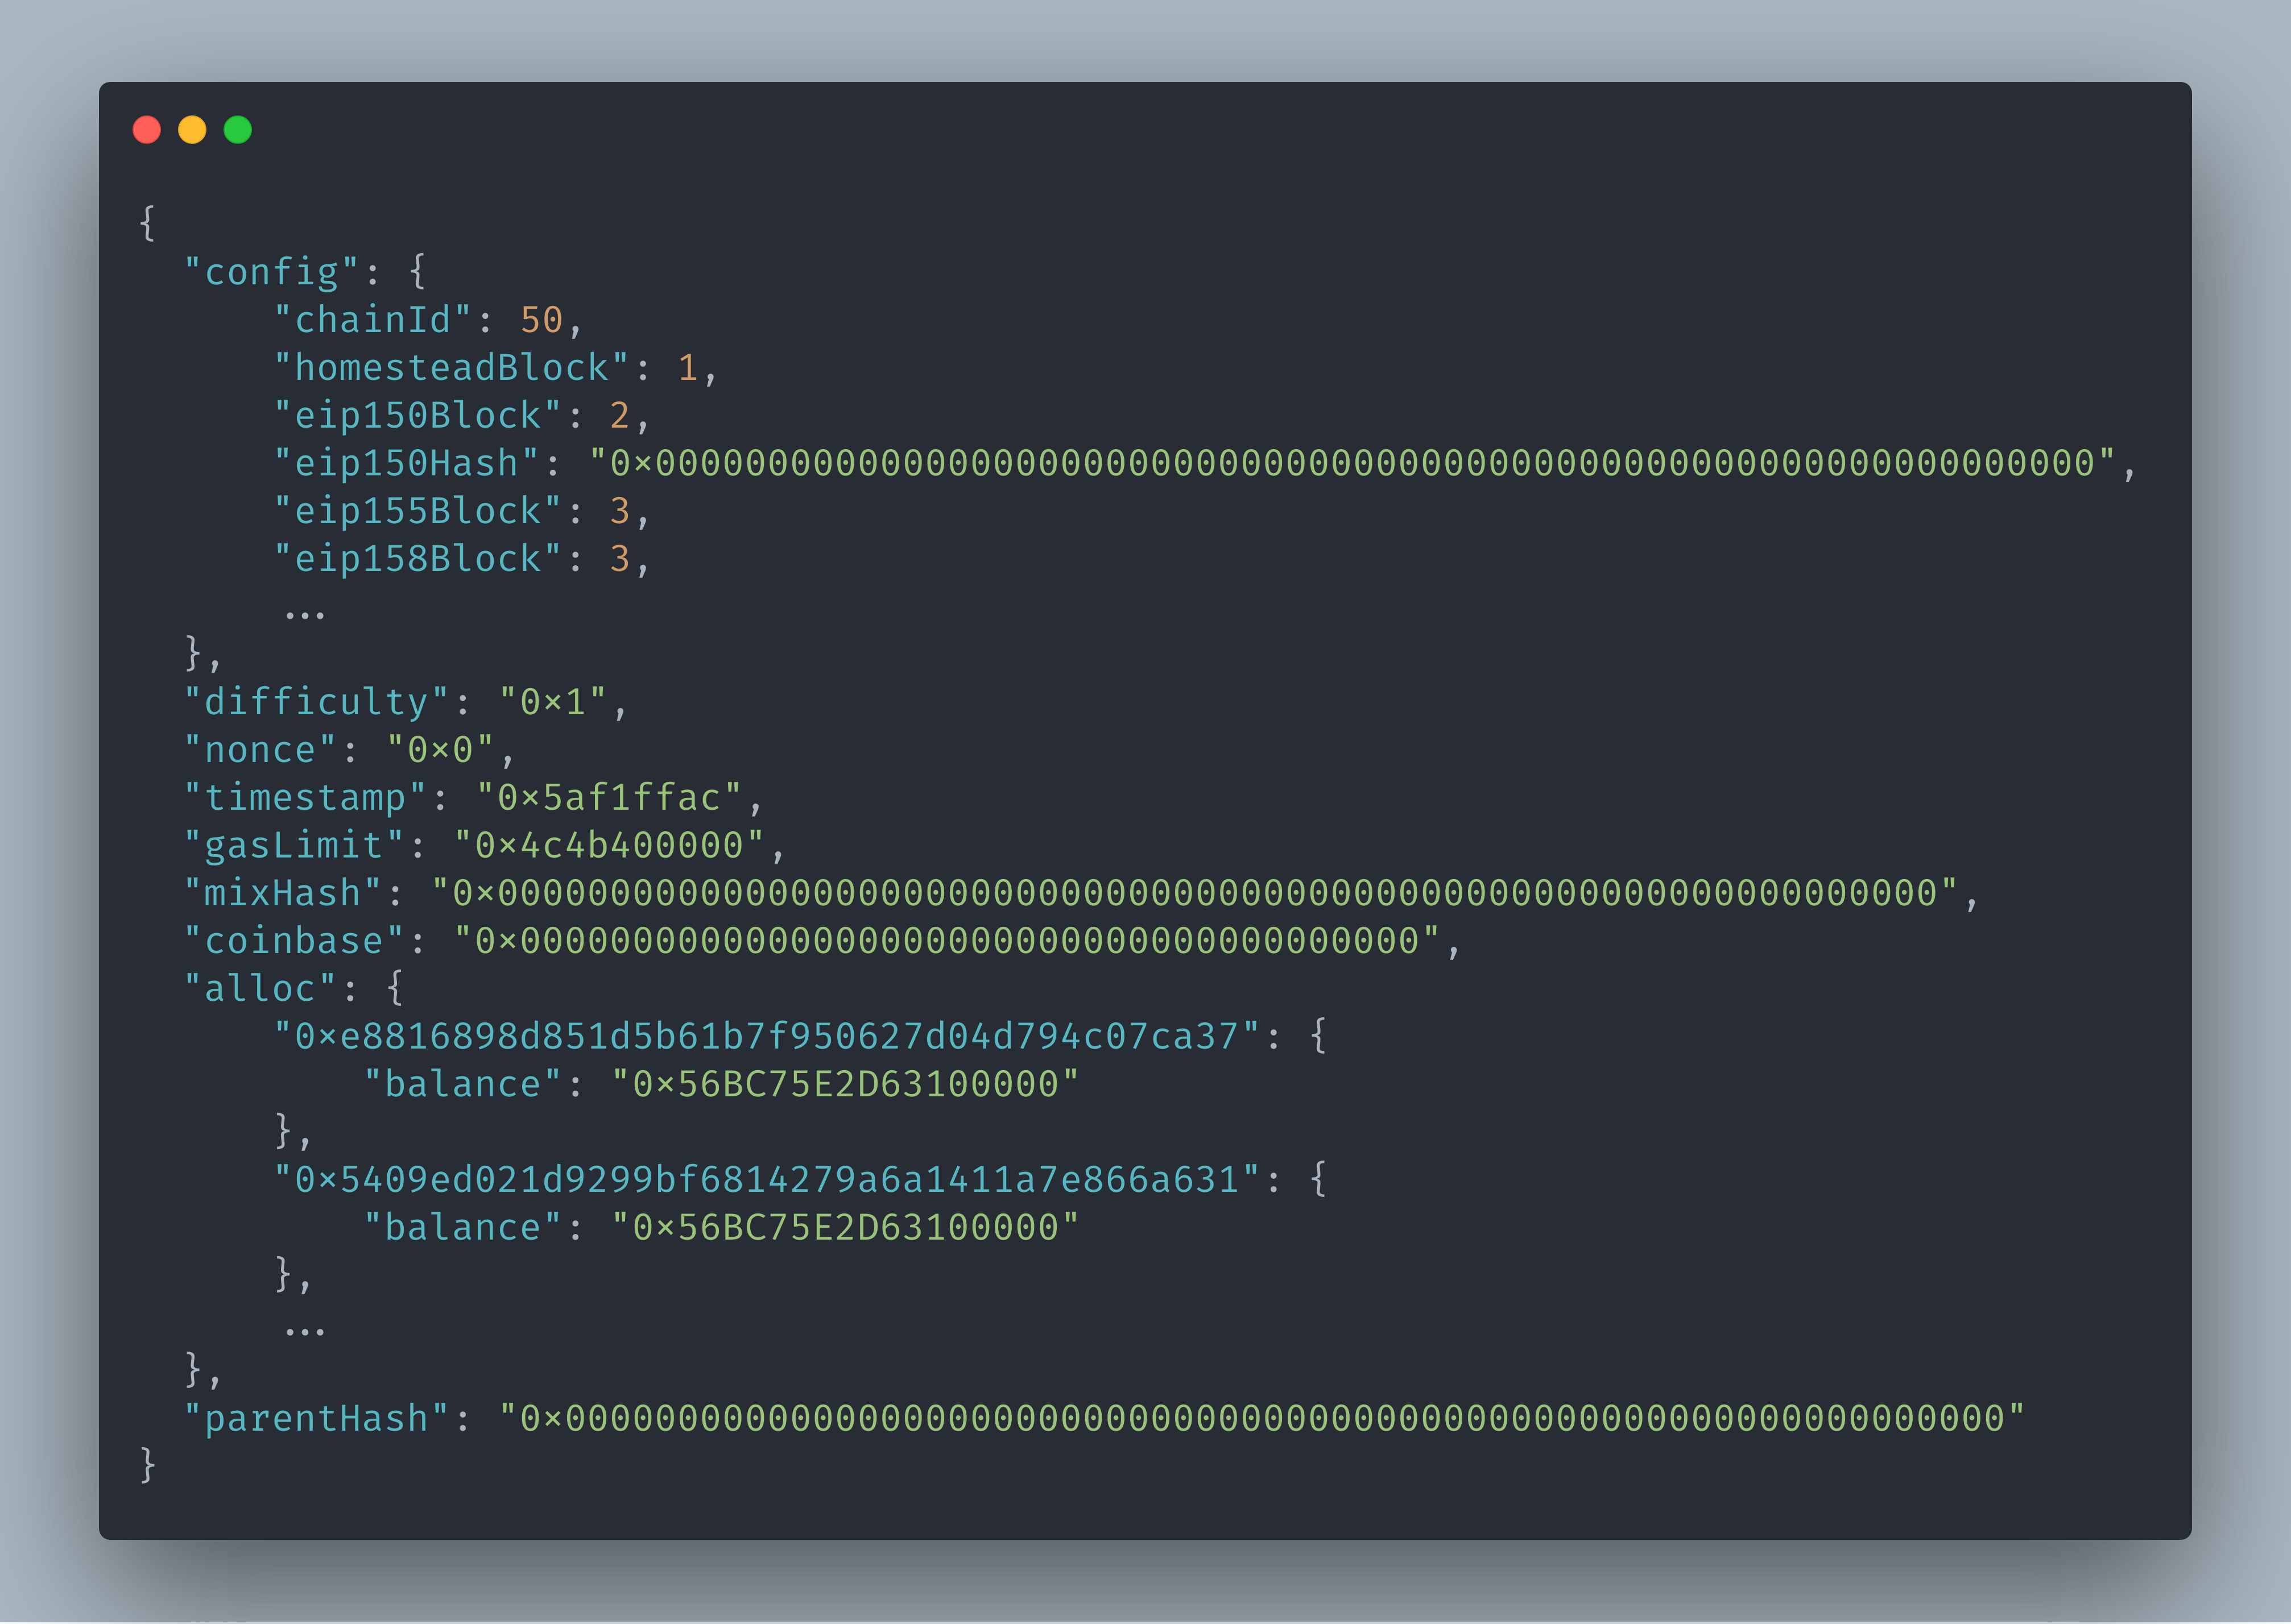
\includegraphics[width=.9\columnwidth]{./Abbildungen/Kapitel_03/genesis.json.png}
	\caption{
		genesis.json\\
		JSON-File welches zur Erstellung des Genesis Blocks verwendet wurde.
	}
	\label{img:gen}
\end{figure}

\begin{itemize}
	\item[-] chainId: ist eine einzigartige Id für die private Blockchain
	      	      	      
	\item[-] eip150Block/eip155Block/eip158Block: eip steht für \quotes{Ethereum Improvement Proposal}. Diese drei Community getriebenen \quotes{Proposals} beschreiben sog. \quotes{hard forks}, welche dafür sorgen sollten Fehler im Protokoll zu beheben. 
	      	      	      
	\item[-] homesteadBlock: Homestead ist die zweite \quotes{major version} von Ethereum, welche einige Änderungen an dem Protokoll vornahm
	      	      	      	
	\item[-] difficulty: beschreibt die Schwierigkeitsstufe für einen Miner einen validen Block zu finden. Das heißt je höher der Wert desto mehr Berechnungen müssen statisch durchgeführt werden und desto mehr Zeit wird benötigt, um eine Transaktion zu bestätigen. Im Falle eines Testnets ist es deshalb ratsam einen sehr niedrigen Wert zu wählen
	      	      	      	
	\item[-] gasLimit: beschreibt das Limit für eine Transaktion wie viel an Gas verbraucht werden darf. 
	      	      	      
	\item[-] alloc: hier können Accounts schon im Voraus mit \quotes{fake ether} befüllt werden.
	\item[-] nonce: ist ein Zähler für die Anzahl der durchgeführten Transaktionen einer Adresse
\end{itemize}

Sobald die genesis.json Datei fertiggestellt ist, kann die Blockchain mit folgendem Befehl erstellt werden:\\\\
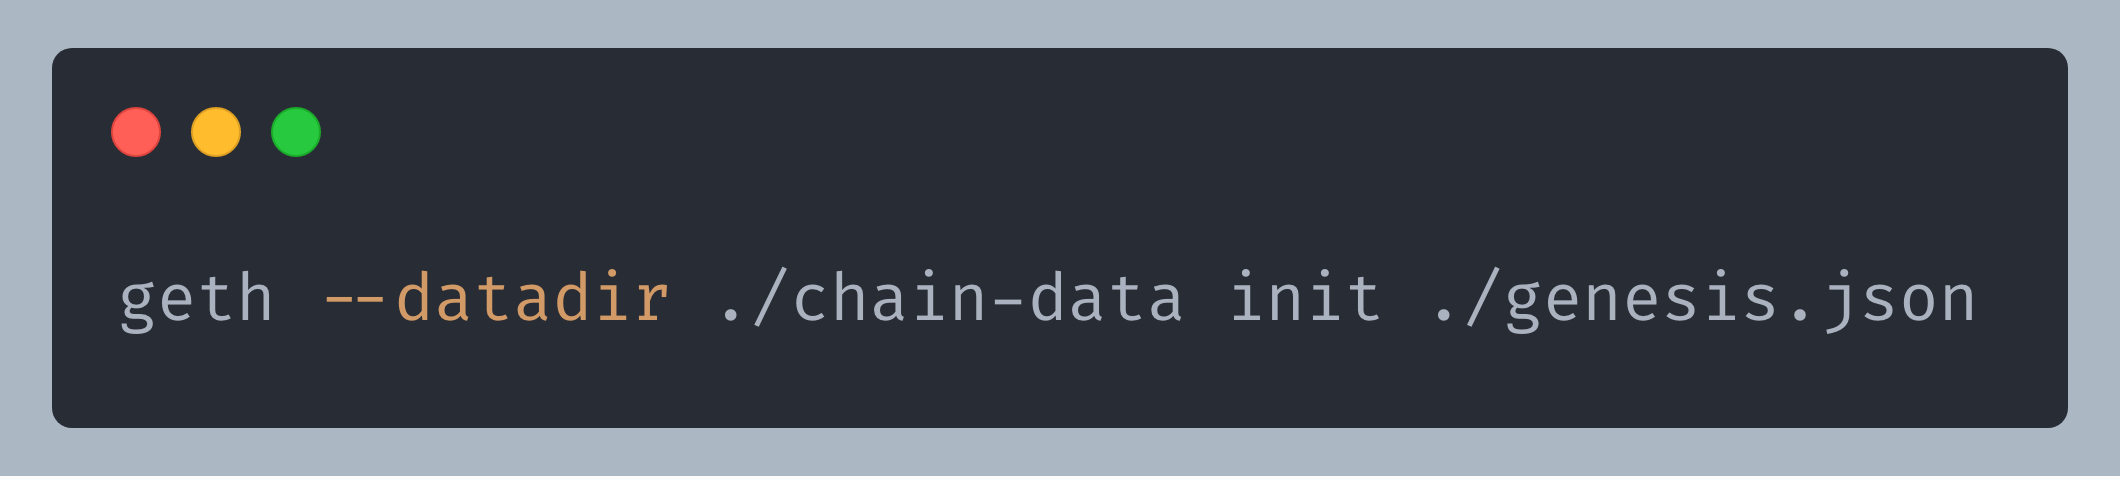
\includegraphics[width=.9\columnwidth]{./Abbildungen/Kapitel_03/geth-init.png}

Das Flag \textit{-{}-datadir} ist mit dem aus Abbildung \ref{img:geth} identisch. Das bedeutet das Verzeichnis welches hier im Befehl angegeben ist, muss beim Kommandozeilenbefehl in Abbildung \ref{img:geth} exakt gleich sein. Andernfalls ist es nicht möglich die Blockchain zu starten.\\\\
Nachdem der Setup der privaten Blockchain abgeschlossen ist, kann mit der Entwicklung eines Smart Contracts begonnen werden. \\
Die nächsten beiden Unterkapitel befassen sich mit den Smart Contracts, welche im Zuge dieser Arbeit entwickelt wurden.

\subsection{CoffeeCoin}
\label{subsec:cc}
Der Smart Contract \quotes{CoffeeCoin} stellt einen sogenannten ERC-20 Token mit gewissen Abwandlungen dar. Dabei ist ein Token im Grunde eine zusätzliche Währung zur eigentlichen Währung von Ethereum dem Ether. Das bedeutet Smart Contracts können somit eine eigenständige Währung abbilden. Für solche Smart Contracts gibt es mittlerweile einige Standardisierungen, die Vorschreiben welche Methoden und Datenstruktur ein Smart Contract zu implementieren hat. Der am weit verbreitetste Standard ist der ERC-20, bei welchem es folgende Funktionen und Events zu implementieren gilt:

\begin{figure}[th!]
	\centering
	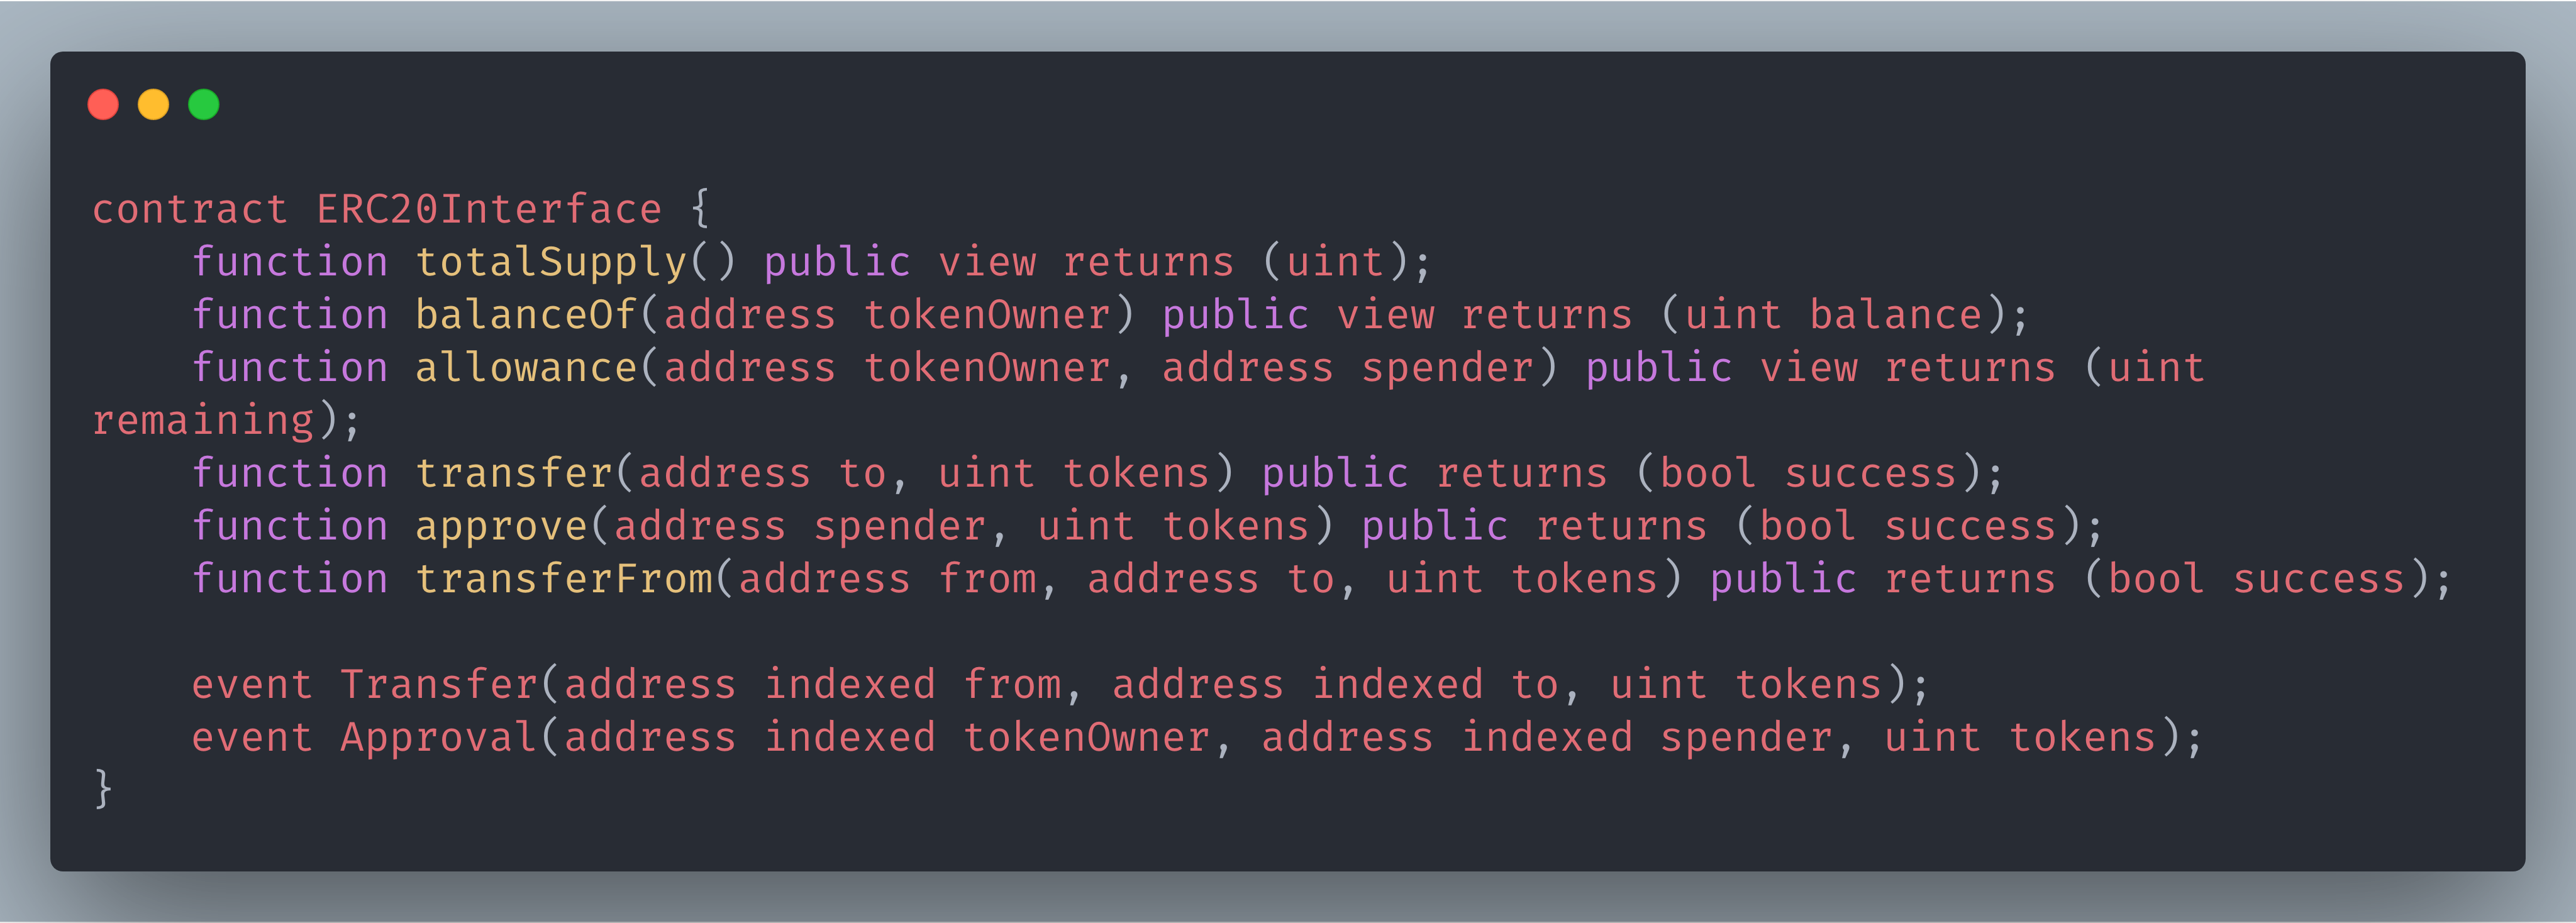
\includegraphics[width=.9\columnwidth]{./Abbildungen/Kapitel_03/erc20.png}
	\caption{ERC-20 Interface}
	\label{img:gen}
\end{figure}

\begin{itemize}
	\item totalSupply: Gesamtanzahl der existierenden Tokens
	\item balanceOf: Anzahl der Tokens eines bestimmten Users
	\item allowance: besagt wie viele Tokens eines bestimmten Users durch einen bestimmten \quotes{spender} abgehoben werden dürfen
	\item transfer: transferiert die Inputanzahl an Tokens des \quotes{senders} (Adresse welche diese Funktion aufgerufen hat) an die angegebene Adresse
	\item approve: Erlaubniserteilung an den \quotes{spender} die in \textit{allowance} festgelegte Anzahl an Tokens abzubuchen
	\item transferFrom: transferiert die angegebene Anzahl von Tokens von der \quotes{from Adresse} zur \quotes{to Adresse}
	\item event Transfer: wird von den beiden \textit{transfer} Funktionen ausgelöst
	\item event Approval: wird von der \textit{approve} Funktion ausgelöst
\end{itemize}

Der eben erläuterte Token Standard wurde im Falle des CoffeeCoin Smart Contracts um zusäztliche Funktionen und Datenstrukturen erweitert. Diese Erweiterungen stellen eine gesonderte Abstraktionsebene nach außen hin da, um die Kommunikation seitens der Tablet-App zu erleichtern und einfacher zu gestalten.\\
So werden schon beim Deployment die einzelnen Preise der Getränke und die Adresse, zu jener die Tokens beim Bezahlen eines Getränks überwiesen werden, gesetzt.\\
Dies ermöglicht die Implementierung folgender Funktionen: 

\begin{figure}[th!]
	\centering
	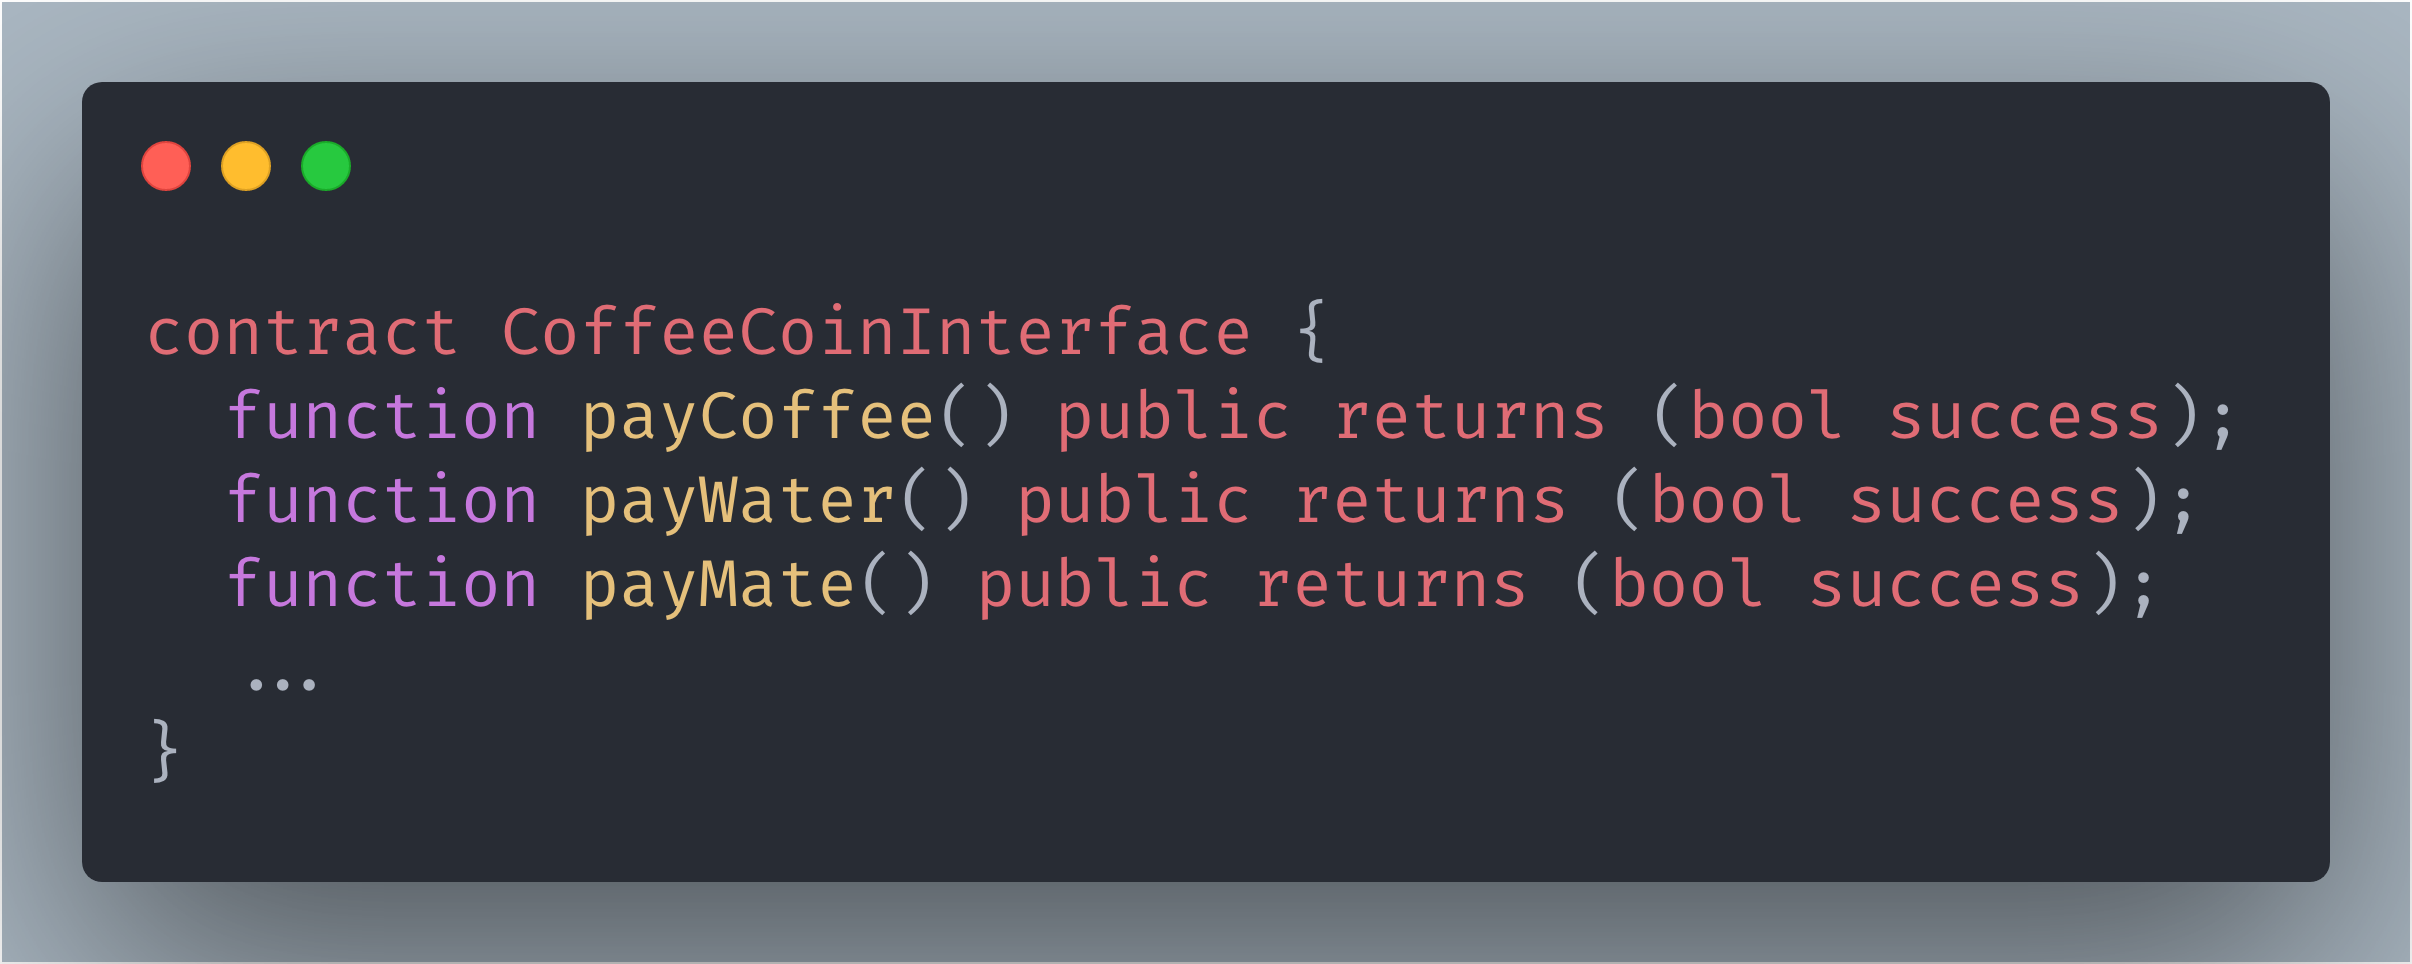
\includegraphics[width=.9\columnwidth]{./Abbildungen/Kapitel_03/CCInterface.png}
	\caption{CoffeeCoin Interface Auszug}
	\label{img:cci}
\end{figure}

Diese Funktionen bieten eine Abstraktionsebene zur ERC-20 Funktion \textit{transferFrom}. Da bereits beim Deployment die Parameter für die Getränke und die Zieladresse gesetzt werden, benötigen diese Funktionen keine weiteren Daten von der Seiten der User (Tablet-App). Somit kann nach Auswahl des Getränks die entsprechende Funktion aufgerufen werden, ohne sich dabei mit den Details der Transaktion beschäftigen zu müssen.\\\\
Desweiteren wird einem User, beim ersten Aufruf einer jener Funktionen (erste ausgelöste Transaktion des Users), eine festgelegte Anzahl an Tokens als \quotes{Startguthaben} überwiesen, sodass dieser stets über genügend Token verfügt und jederzeit Transaktionen durchführen kann.\\
Im Kontext der Problemstellung liegt die Zweckmäßigkeit des Smart Contracts grundsätzlich in der Bezahlung der Getränke in Form des Tokens. Dabei soll vor allem die Möglichkeit einer solchen Bezahlmethode aufgezeigt werden, weswegen die Transaktionen lediglich auf exemplarischer Ebene durchgeführt werden. Das bedeutet, den Usern wird, wie gerade beschrieben, eine nahezu unendliche Menge an Tokens zugewiesen ohne eine Gegenleistung zu fordern.\\\\
Der Sourcecode ist im Anhang unter REF SO UND SO zu finden.


\subsection{Beverage-List}
\label{subsec:bl}

Im Gegensatz zur CoffeeCoin basiert der Beveragelist Contract auf keinem festgelegten Standard, sondern ist in voller Gänze an die Problemstellung angepasst.\\
Dessen Zweck besteht im Grunde darin eine Getränkeliste abzubilden, in welcher jede Getränktransaktion eines Users vorzufinden ist. Dabei wird pro Transaktion nicht nur das Getränk, sondern auch das aktuelle Datum inklusive Uhrzeit und der aktuelle Wochentag, gespeichert. Diese Daten sollen es dem Learner schlussendlich ermöglichen das Kaffeetrinkverhalten des Users zu erlernen. \\
Damit der Learner ohne großen Aufwand auf diese Informationen zugreifen kann, löst der Smart Contract, mit den eben genannten Daten beinhaltend, ein Event aus, sobald seine Methode \quotes{setDrinkData} aufgerufen wird. Diese Funktion 
hinterlegt die übergebenen Daten (Eth-Adress, Zeit, Wochentag, Getränk) in festgelegten Datenstruktur und löst zugleich das Event für den Learner aus.\\\\

Dieser Smart Contract umfasst noch weitere Funktionen, welche aber vor allem zu Testzwecken implementiert wurden und in der finalen Systemarchitektur keine Verwendung finden. 


\section{Learner}
\label{sec:ql}
Als nächstes wird der sogenannte \quotes{Learner} detailiert betrachtet. Dabei wird zuerst die Problemstellung hinsichtlich des Reinforcement-Learnings modelliert und im Anschluss der verwendete Algorithmus (Q-Learning) allgemein und im Kontext der Problemstellung erläutert. \\

\subsection{Modellierung}
\label{subsec:modulation}
Die Modellierung eine Lernproblems im Hinblick auf einen Reinforcement-Algorithmus erfolgt in der Regel stets nach der selben Systematik. \\
Dabei werden zuerst der Zustandsraum, also alle möglichen Zustände, alle Aktionen des \quotes{Agenten} und der Reward für ausgeführte Aktionen eruiert.
Hier in diesem Fall ist der Agent der Learner, welcher das Kaffeetrinkverhalten der User zu erlernen versucht.\\\\
Die Modellierung sieht wie folgt aus: 
\paragraph{Zustandsraum}
\begin{itemize}
	\item Wochentag: Montag, Dienstag, Mittwoch, Donnerstag, Freitag
	\item Timeslot:
	      \begin{itemize}
	      	\item 7-9 Uhr (T0)
	      	\item 10-12 Uhr (T1)
	      	\item 13-15 Uhr (T2)
	      	\item 16-18 Uhr (T3)
	      	\item 19-6 Uhr (T4)
	      \end{itemize} 
	\item Kafee-Anzahl: n $*$ Kaffee (n=Anzahl pro Tag)
\end{itemize}

\paragraph{Aktionen}
\begin{itemize}
	\item Kaffee
	\item Nothing
\end{itemize}

\paragraph{Reward}
\begin{itemize}
	\item +1 bei richtiger Prediction
	\item \textminus 1 bei falscher Prediction
\end{itemize}
\ \\
Daraus lässt sich folgender examplarischer Zustand konstruieren: 
\begingroup
\makeatletter
\@totalleftmargin=0.5cm
\begin{Verbatim}
< Wochentag: Montag; Timeslot: 2; Kaffee-Anzahl: 3 >
\end{Verbatim}
\endgroup
Das bedeutet konkret: an einem Montag wurden einschließlich des 2. Timeslots (13-15 Uhr) 3 Kaffee getrunken. Dieser Status gibt jedoch keinen Aufschluss darüber, welcher sein Vorgänger war und welcher sein Nachfolger sein wird. So können einerseits alle Kaffee's nur in Timeslot 2 getrunken worden sein oder in jedem Timeslot (0,1,2) jeweils einen. Andererseits besteht auch die Möglichkeit, dass im Timeslot 2 nochmals ein Kaffee konsumiert wird oder eben erst in einem nachfolgendem Timeslot.\\
Dieses Lernproblem ist auch als \quotes{Multi-Armed Bandit Problem} bekannt und wird in Kap. \ref{subsec:y-ql} erläutert.
\\\\
Der erste Modellierungansatz sah anstatt der Kaffe-Anzahl eine Getränkeanzahl vor, bei der zum Kaffee auch die Quantität der getrunkenen \quotes{Clube Mate} und \quotes{Wasser} berücksichtigt werden sollten. Der Grund dafür liegt in dem erheblichen Einfluss des Konsums weiterer Getränke auf das Kaffeetrinkverhalten, wodurch mit solch einer granulareren Modellierung genauere Predictions zu erwarten sind. Jedoch steigt somit auch die Anzahl der zu durchlaufenden Zustände und einhergehend damit die zu erlernenden optimalen Aktionen für die Zustandsübergänge. Letzlich resultiert dies in der längeren Trainingsphase des Algorithmus, was aber aufgrund des zeitlich begrenzten Rahmen dieser Arbeit nicht durführbar war und deshalb der Ansatz mit lediglich der Kaffee-Anzahl gewählt wurde.\\

TO-DO: feature selection to add
user versteht zu jeder warum algorithmus so handelt

\subsection{Q-Learning}
\label{subsec:y-ql}
Im folgenden wird der implementierte Q-learning Algorithmus zuerst allgemein und anschließend im Bezug auf die Problemstellung erläutert.\\
TO-DO: Alles!!!! \\

\subsection{Lernprozess \& Ablauf}
\label{subsec:learning}

Aufgrund der Modellierung eines Zustandes ergeben sich zwei Arten bei denen eine Änderung dessen hervorgerufen wird: 
\begin{itemize}
	\item durch eine zeitliche Komponente, bei der sich entweder der Timeslot oder der Tag ändert
	\item durch den User indem er eine Transaktion auslöst
\end{itemize}

Das ist in der Hinsicht von großer Bedeutung, da für diese Übergänge ein Feedback für den Agenten notwendig ist, um jeweils die optimale Aktion dafür zu erlernen. \\
So wird das Feedback einerseits von Seiten des Users in Form einer bestätigten Transaktion generiert, was bedeutet Aktion \quotes{Kaffee} wurde ausgeführt. Oder andererseits als Folge einer fehlenden Rückmeldung des Nutzers, welche \quotes{Nothing} als optimale Aktion impliziert. \\
Das heißt erfolgt eine Zustandsänderung durch den User, so ist stets \quotes{Kaffee} die zu erlernende, beste Aktion. Wird eine Zustandsänderung durch einen Timeslotwechsel bewirkt, so ist das Feedback der Umgebung immerfort die Aktion \quotes{Nothing}. \\
Um dem Agenten bzw. dem Q-Learning Algorithmus stets das nötige Feedback zu geben und Zustandsübergänge herbeizuführen, werden im Learner die Komponenten \quotes{Watcher} und \quotes{Worker} verwendet. \\
Der \quotes{Watcher} ist dafür zuständig das Feedback des Users durch das Beveragelist-Event zu detektieren und die darin enthaltenen Daten dem Algorithmus zur Verfügung zu stellen. \\
Der \quotes{Worker} wird für die zeitliche Komponente verwendet, indem er am Ende jedes Timeslots aktiv wird, die Zustandsänderung durchführt und dem Agenten die Aktion \quotes{Nothing} als Feedback gibt. \\
Auf Basis dieser Feedbacks wird es dem Q-Learning Algorithmus ermöglicht die optimalen Aktionen zu erlernen. Hierbei wird die Prediction, also die aus Sicht des Agenten beste Aktion für den Zustandsübergang, anhand der Rückmeldung, sei es durch den Watcher oder Worker, evaluiert und für den nächsten Übergang eine neue Aktion eruiert. \\
Dieses Prinzip der Evaluierung und Vorhersage der Aktion kann im Kontext des Lernproblems jedoch nicht kontinuierlich angewendet werden. 
So bedingen bestimmte Zustände nur eine Evaluierung oder nur eine Vorhersage, indes nie beides. Der Grund hierfür liegt in der Abgeschlossenheit der Tage als Lernabschnitt, welche komplett unabhängig voneinander agieren. \\
Zudem werden die Uhrzeiten zwischen 19 und 6 Uhr (T4) nicht in der Zustandsraummodiellerung berücksichtigt, da in diesem Zeitraum keine Aktion durch den User zu erwarten ist.\\ 
Dies hat für den \quotes{Worker} zur Folge, dass zum einen am Anfang jedes Tages bzw. beim Wechsel von T4 auf T0, lediglich eine Vorhersage für den nächsten Zustandsübergang gemacht und zum anderen am Ende von T3 einzig die letzte Vorhersage evaluiert werden muss.\\\\
Dies lässt sich veranschaulicht folgendermaßen darstellen:
\begin{itemize}
	\item Evaluierung \& Vorhersage: 
	\begin{itemize}
		\item User führt Transaktion durch
		\item Timeslot wechselt
	\end{itemize}
	\item Evaluierung:
	\begin{itemize}
		\item am Ende von T3
	\end{itemize}
	\item Vorhersage:
	\begin{itemize}
		\item am Anfang von T0
	\end{itemize}
\end{itemize}    


\section{Tablet-App}
\label{sec:app}

Das folgende Unterkapitel befasst sich mit dem Aufbau und der Funktionsweise der App und schildert zudem den verwendeten Algorithmus, welcher die Getränk- und Userdaten auf die Blockchain schreibt.\\\\
Die entwickelte App basiert auf dem Crossplattform Framework \quotes{React Native} \cite{RN:ReactNative}, dieses erlaubt es mit einer einzigen Codebasis Apps für unterschiedliche Plattformen (z.B. iOS, Android) zu entwickeln. Der wesentliche Vorteil allerdings liegt in der Verfügbarkeit einer offiziellen Library, mit der es erst möglich ist eine Verbindung zur Blockchain bzw. den Smart Contracts herzustellen. Diese Library (Web3.js) wurde von Ethereum dafür entwickelt, um sog. DApp's (\quotes{decentralized apps}) \cite{DApp} auf Basis von Javascript erstellen zu können. \\
So ist die Entwicklung einer DApp in einer nativen Programmiersprache (Java/Kotlin/Swift) bisher nur mit \quotes{third-party libraries} möglich, weswegen die Umsetzung letztlich mit ReactNative erfolgte.

\subsection{Interface}
\label{subsec:interface}
Eine essentielle Eigenschaft von ReactNative ist der komponentenbasierte Ansatz. Dabei setzt sich eine App aus vielen einzelnen Komponenten zusammen, welche jeweils einen dedizierten Aufgabenbereich abdecken. \\
Im Falle der entwickelten App existieren jeweils zwei \quotes{page components}, die wiederum mehrere kleine Komponenten in sich vereinen. 
Da es aber den Rahmen dieser Arbeit sprengen würde auf jede einzelne Komponente und deren Funktionsweise einzugehen, werden nur die Hauptkomponenten anhand ihrer Funktion und Bedienung geschildert. \\\\
Wird die App gestartet und es besteht eine Verbindung zum Internet bzw. zur Blockchain, so findet der User folgende Startseite vor: 

\begin{figure}[th!]
	\centering
	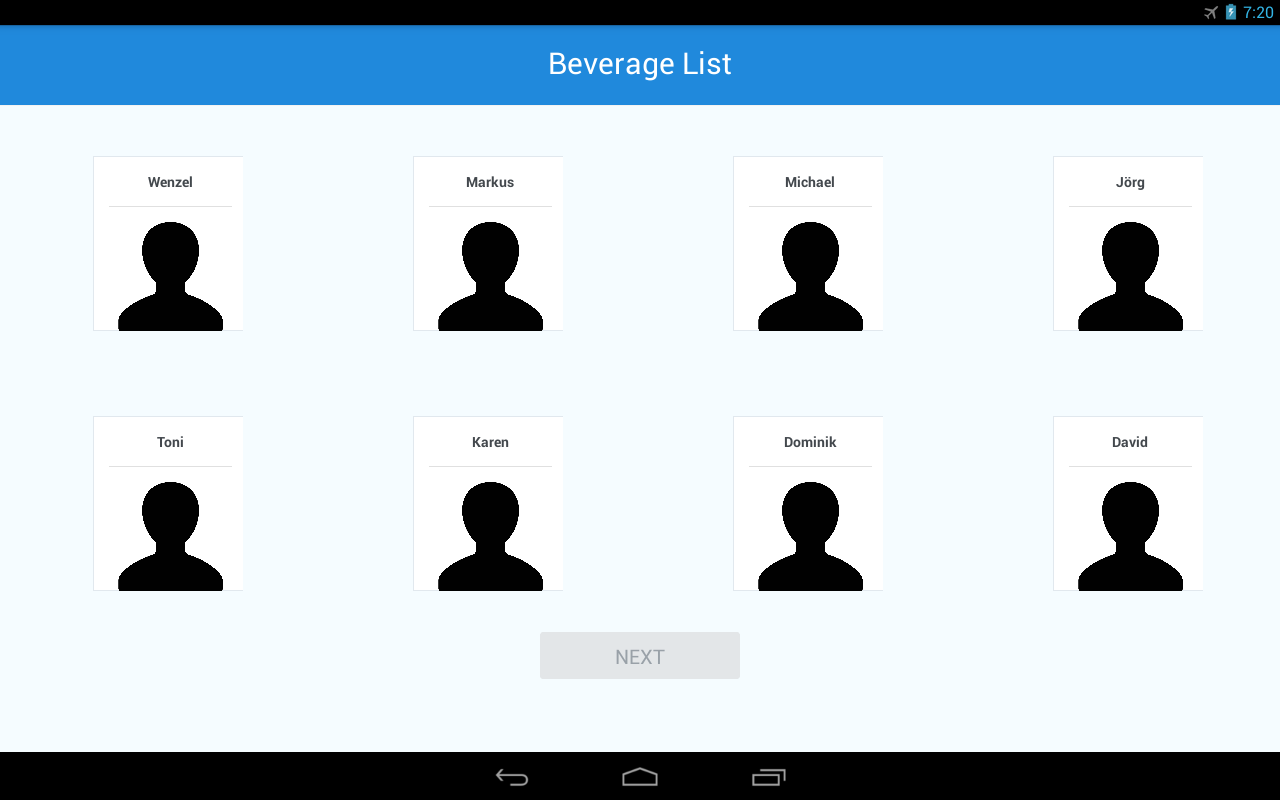
\includegraphics[width=.9\columnwidth]{./Abbildungen/Kapitel_03/emps1.png}
	\caption{Mitarbeiter Page: kein Mitarbeiter ausgewählt}
	\label{img:emps1}
\end{figure}

\begin{figure}[th!]
	\centering
	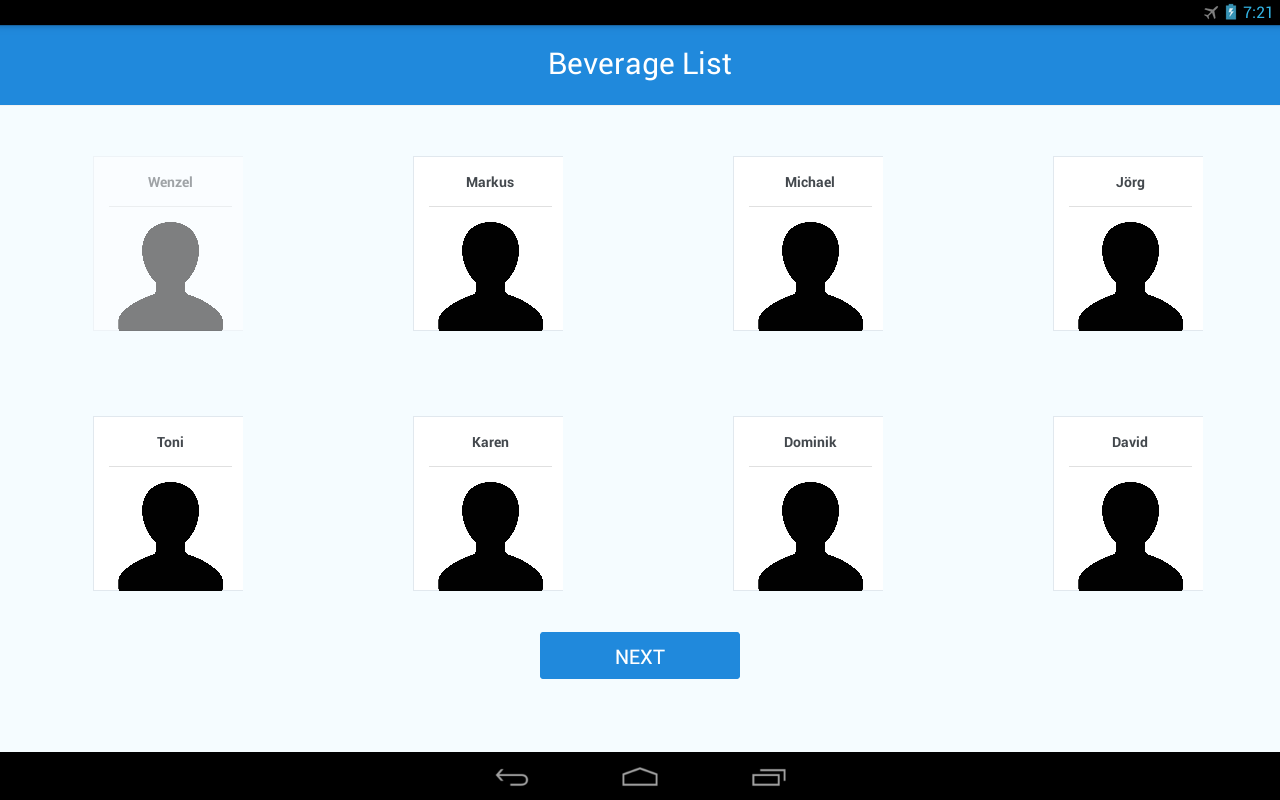
\includegraphics[width=.9\columnwidth]{./Abbildungen/Kapitel_03/emps2.png}
	\caption{Mitarbeiter Page: Mitarbeiter ausgewählt}
	\label{img:emps2}
\end{figure}

Hier kann der User seinen Avatar selektieren und deselektieren. Ist ein Avatar ausgewählt wird der \quotes{NEXT} Button aktiviert (vgl. Abbildung \ref{img:emps2}) und durch dessen Betätigung gelangt der User zur nächsten Seite: 

\begin{figure}[th!]
	\centering
	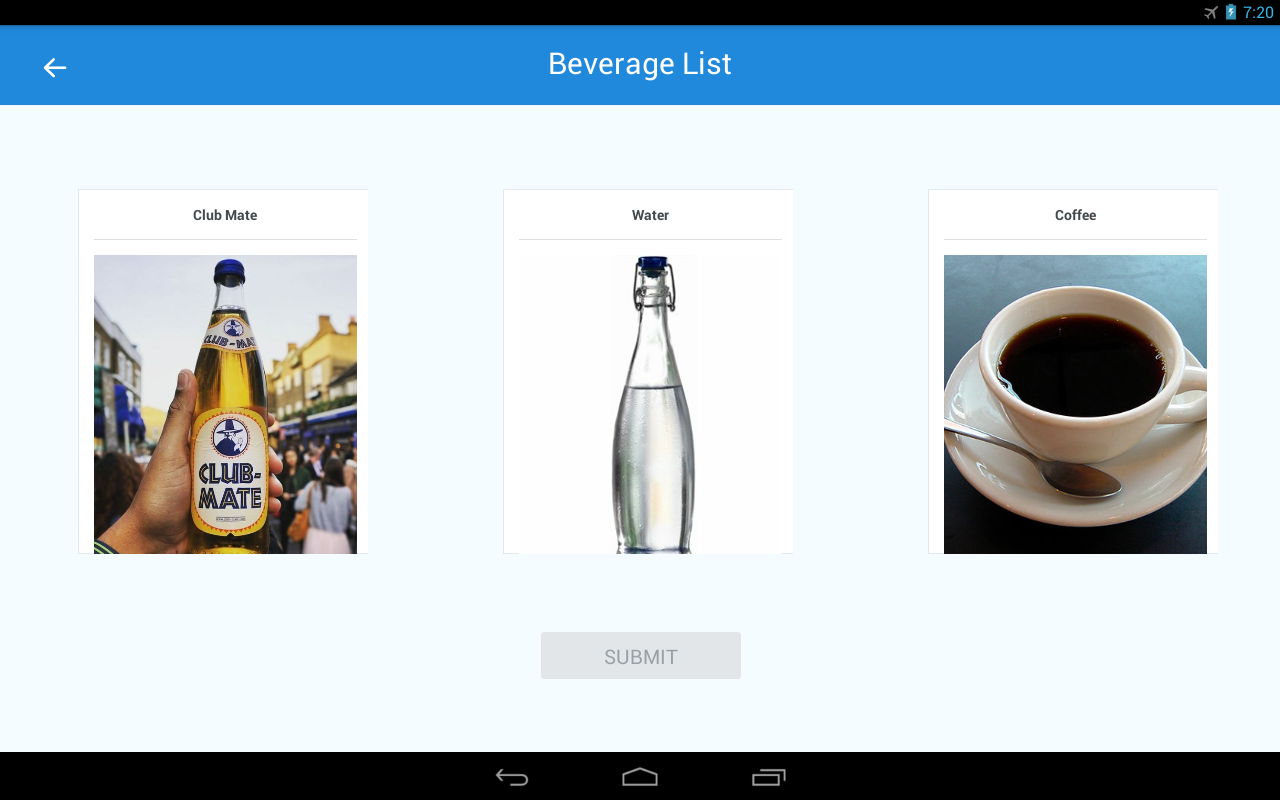
\includegraphics[width=.9\columnwidth]{./Abbildungen/Kapitel_03/drinks1.png}
	\caption{Drinks Page: kein Getränk ausgewählt}
	\label{img:drinks1}
\end{figure}

Hier besteht eine Auswahl aus folgenden Getränken: Club Mate, Wasser und Kaffee. 
Ausgewählt kann jedoch immer nur eines werden (vgl. Abbildung \ref{img:drinks2}).
Das Prinzip der Selektion und Deselektion ist identisch mit dem der vorherigen Seite. So wird der \quotes{SUBMIT} Button aktiv, sobald ein Getränk ausgewählt ist und inaktiv wenn das Getränk wieder deselektiert wird (vgl. Abbildung \ref{img:drinks1}).\\

\begin{figure}[th!]
	\centering
	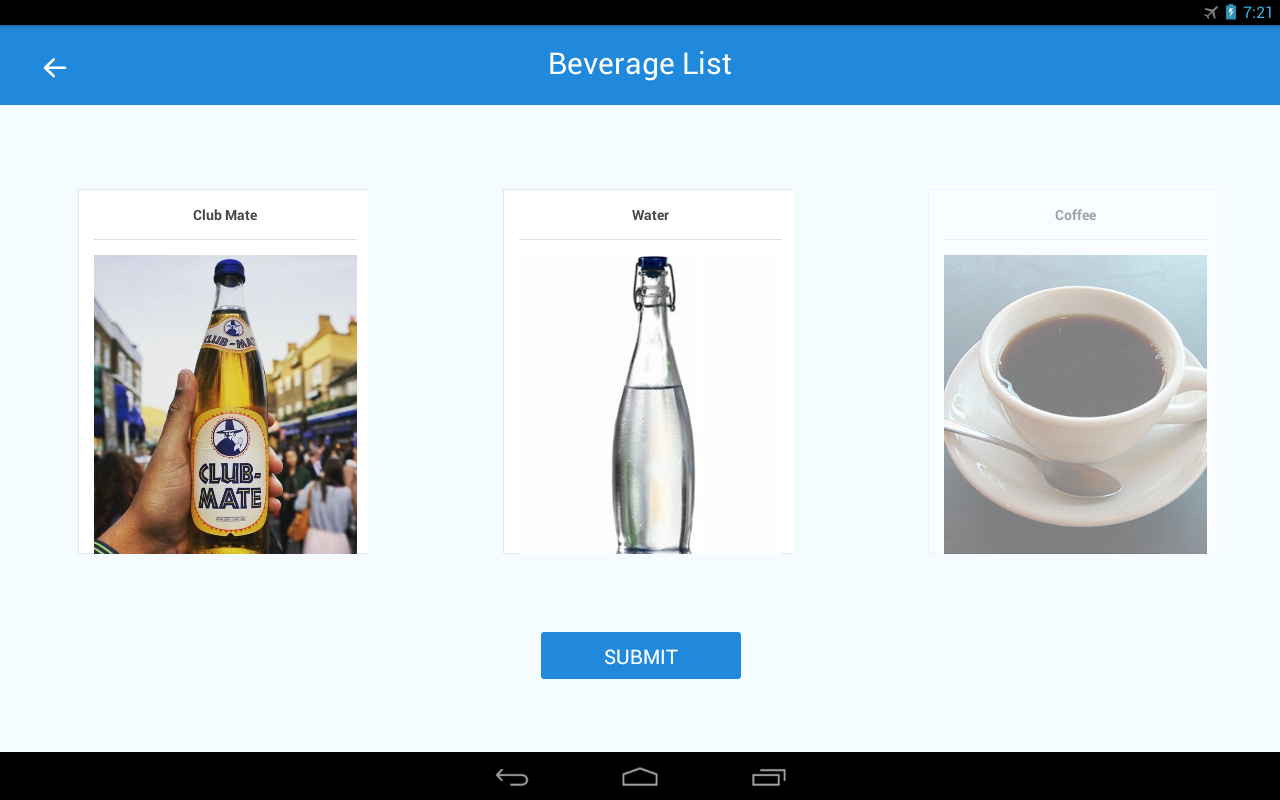
\includegraphics[width=.9\columnwidth]{./Abbildungen/Kapitel_03/drinks2.png}
	\caption{Drinks Page: Getränk ausgewählt}
	\label{img:drinks2}
\end{figure}

Wird schließlich der \quotes{SUBMIT} Button gedrückt und die Transaktion als erfolgreich bestätigt erscheint folgendes Overlay:

\begin{figure}[th!]
	\centering
	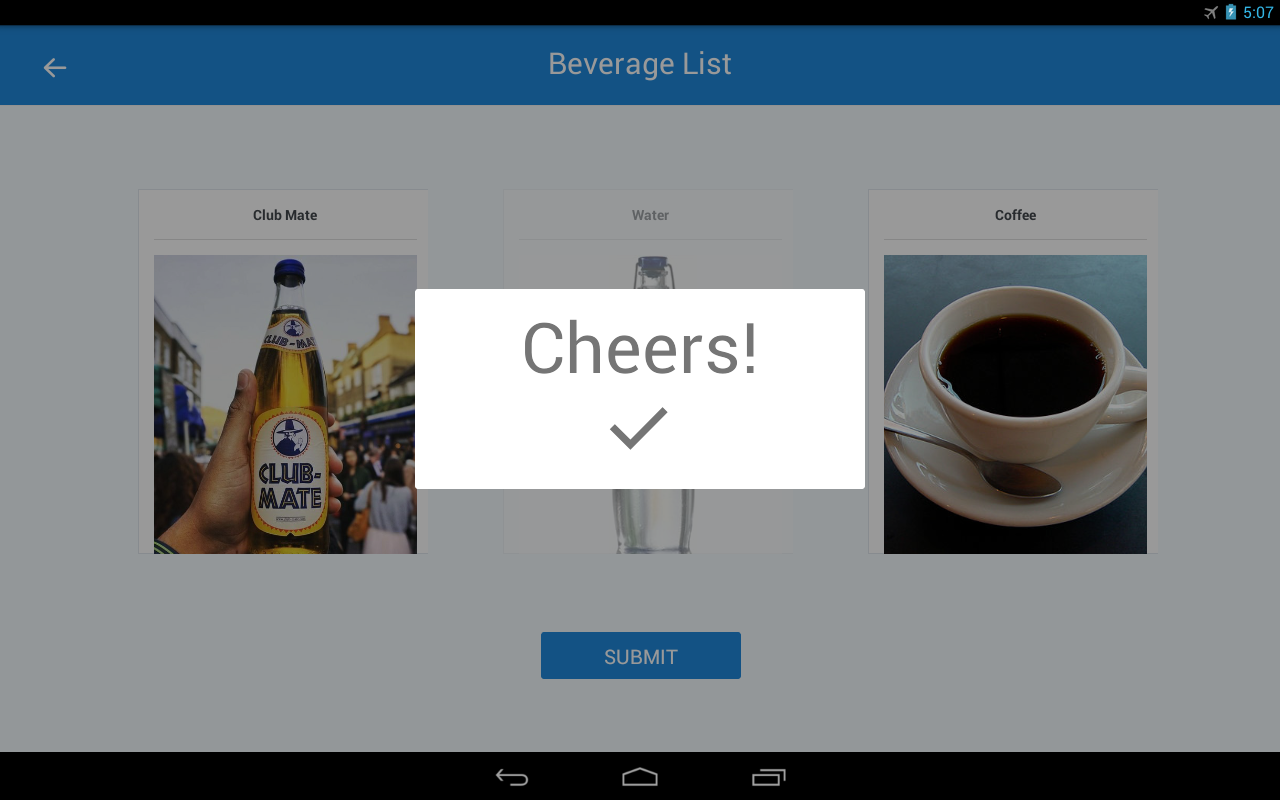
\includegraphics[width=.9\columnwidth]{./Abbildungen/Kapitel_03/cheers.png}
	\caption{}
	\label{img:drinks2}
\end{figure}

Nach 4 Sekunden wird dieses Overlay wieder ausgeblendet und automatisch zur Startseite (vgl. Abbildung \ref{img:emps1}) navigiert, wodurch der Workflow von neuem startet.\\\\
Aufgrund der Tatsache, dass die Verbindung zum Uni-Netzwerk (eduroam) nur über einen Workaround hergestellt werden konnte, bei dem die Verbindung zum Netzwerk trotzdessen nach einer unbestimmten Zeit immer wieder abgebrochen ist, wurde eine weitere Komponente entwickelt.

\begin{figure}[th!]
	\centering
	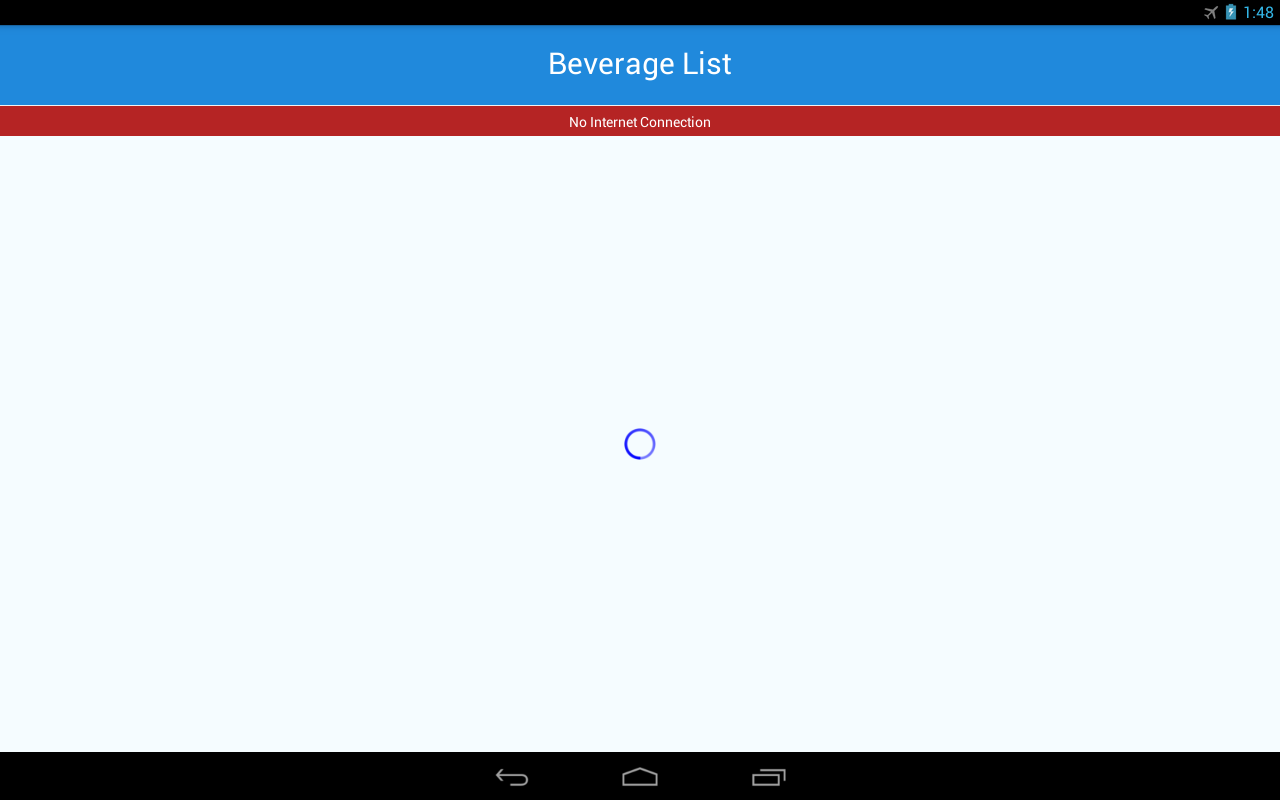
\includegraphics[width=.9\columnwidth]{./Abbildungen/Kapitel_03/noconnection.png}
	\caption{}
	\label{img:drinks2}
\end{figure}

Diese wird sofort eingeblendet sobald die Verbindung zum Internet unterbrochen ist, allerdings nur wenn sich der User auf der Startseite befindet. Wird die Seite mit den Getränken angezeigt, so wird dem User die Möglichkeit gegeben seine Transaktion abzuschließen. Da in diesem Moment jedoch keine Verbindung zur Blockchain hergestellt werden kann, werden die Transaktionsdaten zwischengespeichert und diese durchgeführt sobald wieder eine Verbindung zum Netzwerk besteht (vgl. Kap. \ref{subsec:internalFlow}).
Die Loading Animation sowie das \quotes{No Internet Connection} Label werden wieder ausgeblendet sobald die App eine erneute Verbindung zum Uni-Netzwerk detektiert.

\subsection{Internal Workflow}
\label{subsec:internalFlow}
Basierend auf der Problematik eines unerwarteten Verbindungsabbruch und dem einhergehenden Verlust von essentiellen Lerndaten, wird im folgenden der implementierte Algorithmus geschildert, der dieser Komplikation entgegenwirkt. 

\begin{legal}
	\item Initialisierungsphase:
	\begin{legal}
		\item \quotes{GET} Smart Contract Daten von Fileserver
		\item Initialisierung Web3.js
		\item Wiederhole für jedes Transaktionsfile:
		\begin{legal}
			\item Transaktion durchführen
			\item bei \quotes{Success} Transaktiondatei löschen
		\end{legal}
	\end{legal}
	\item Warten auf Usereingabe:
	\begin{legal}
		\item User ausgewählt $\rightarrow$ Ethereum-Adresse
		\item Getränk ausgewählt $\rightarrow$ Getränk
		\item Submit $\rightarrow$ (Getränk \& Ethereum-Adresse)
	\end{legal}
	\item Wiederhole für jedes User-Transaktionsfile:
	\begin{legal}
		\item Transaktion durchführen
		\item bei \quotes{Success} Transaktiondatei löschen
	\end{legal}
	\item Generierung Transaktionsdaten:
	\begin{itemize}
		\item Gas Estimate
		\item Datum (inkl. Zeit)
		\item Wochentag
		\item Ethereum-Adresse \& Getränk aus 2.3
	\end{itemize}
	\item Transaktion starten:
	\begin{legal}
		\item Erstellung der Transaktiondatei
		\item Transaktion durchführen
		\item bei \quotes{Success} Transaktiondatei löschen
		\item gehe zu 1.
	\end{legal} 	
\end{legal}

Der interne Workflow beginnt mit der Initialisierungsphase, dabei werden zuerst die Smart Contract Files vom Fileserver runtergeladen und mit den beinhaltenden Daten das Web3.js Modul initialisiert. Damit steht Verbindung und die Kommunikation mit den Smart Contracts und es wird im Anschluss über alle vorhandenen Transaktion Files iteriert. Dabei wird zuerst der CoffeeCoin Contract und dann der Beveragelist Contract aufgerufen. Wenn beide ihre Transaktionen bestätigt haben, wird die Datei gelöscht, andernfalls bleibt diese bestehen. Dies geschieht noch bevor der User das Interface zu Gesicht bekommt.\\\\
Nachdem 1. abgeschlossen ist wird auf die Eingabe des Users gewartet. Wählt dieser einen Avatar aus klickt \quotes{NEXT} wird seine hinterlegte Ethereum-Adresse temporär gespeichert. Wird dann im Anschluss ein Getränk selektiert und \quotes{SUBMIT} gedrückt, werden die Ethereum-Adresse und das Getränk an das interne Blockchain-Modul weitergereicht und die Transaktion gestartet. \\\\
Dabei wird erneut über die Transaktionsdaten iteriert, allerdings nur über die des Users. Damit soll stets die richtige Reihenfolge der getrunkenen Getränke sichergestellt werden, da dies ansonsten auf Seiten des Q-Learning Algorithmus zu falschen Lerneffekten führen würde.\\\\
Daraufhin kann mit der Generierung der fehlenden Transaktionsdaten angefangen werde. Es wird zuerst ein \quotes{Gas Estimate} für beide Smart Contract Transaktionen durchgeführt. Ein \quotes{Gas Estimate} ist, wie der Name bereits impliziert, eine grobe Schätzung wie viel Gas beim Funktionsaufruf eines Smart Contracts benötigt wird. Abschließend werden das Datum (inkl. Zeit in Sekunden) und der Wochentag ermittelt und alle benötigten Daten an die jeweiligen Smart Contract Funktionsaufrufe übergeben. Im Falle des Smart Contracts Beveragelist: \textit{Gas-Estimate, Datum, Wochentag, Ethereum-Adresse, Getränk}.
Bei CoffeeCoin wird anhand des Getränks die entsprechende Smart Contract Funktion ausgewählt und lediglich das \textit{Gas-Estimate} und die \textit{Ethereum-Adresse} des Users übergeben.\\\\
Bevor jedoch beide Transaktionen durchgeführt werden, wird ein Transaktionsfile mit dem Namen \quotes{<<ethereum-adresse>>-<<datum>>.json} und den Daten \textit{Datum, Wochentag, Ethereum-Adresse, Getränk} gespeichert. Sogleich werden beide Funktionsaufrufe getätigt und bei erfolgreicher Bestätigung beider Transaktionen wird das gerade erstellte File wieder gelöscht. Somit soll sichergestellt werden, dass keine Transaktionen aufgrund von Verbindungsabbrüchen verloren gehen. \\\\
Anschließend erfolgt eine \quotes{Pseudo-Reload} der App und der Ablauf beginnt wieder bei 1.
\chapter{Studie}
\label{kap:Kapitel04}

\section{Simulation}
Die Simulation ist die Grundlage der Evaluation der durchgeführten Studie. Sie soll in erster Linie zeigen, dass die Implementierung des Q-Learning Algorithmus fehlerfrei funktioniert und es für einen Agenten damit möglich ist das Verhalten eines Nutzers zu erlernen. \\
Dazu bedarf es allerdings Testdaten welche das Kaffeetrinkverhalten eines Users repräsentieren. Im \quotes{Simulator} wird es wie folgt umgesetzt.\\
Abstrakt gesehen wird ein virtueller User anhand von Zufallszahlen einer Normalverteilung simuliert.\\
Genauer betrachtet werden die Zeiten, an denen dieser virtuelle User einen Kaffee trinkt, basierend auf der Ziehung von Zahlen aus einer Normalverteilung erzeugt.\\ Dabei wird pro Tag (Montag-Freitag) und in jedem Timeslot (T0-T4) unter Berücksichtigung einer vordefinierten Abweichung und Erwartungswert (siehe \ref{tab:meandevtable}), die Anzahl der getrunkenen Kaffees ermittelt. Für jeden Kaffee wird zufällig eine Uhrzeit gezogen, welche sich in dem Zeitraum des Timeslots befindet. Somit wird ein Trainingsset für den Agenten erstellt, welches das Verhalten einer realen Person in einem Zeitraum von einer Woche abbildet.

\begin{center}
    \captionof{table}{Normalverteilung Tabelle}
    \label{tab:meandevtable}
    \begin{tabular}{| l | l | l |}
    \hline
    Timeslot & Erwartungswert & Abweichung \\ \hline
    0 & 1,0 & 1,0 \\ \hline
    1 & 1,5 & 0,2 \\ \hline
    2 & 1,5 & 0,01 \\ \hline
    3 & 0,2 & 0,5 \\ \hline
    4 & 0,0 & 0,0 \\ \hline
    \end{tabular}
\end{center}


Der Pseudocode des Simulators sieht folgendermaßen aus (vgl. Algorithmus \ref{algo:sim}):

\begin{algorithm}
    \caption{Simulation algorithm}\label{algo:sim}
    \begin{algorithmic}[1]
    \State \emph{weeks} $\gets$ x   \hfill         //x = Anzahl der Episoden
       \For{weeks}
       \State \emph{trainSet} $\gets$ $generateTrainingsSet()$
       \For{$1 \leq day \leq 6$}    \hfill         //Montag-Freitag
       \For{$7 \leq ts < 19$}       \hfill         //Timeslot 0-4
       \State \emph{times} $\gets$ $trainSet[\emph{day}][\emph{ts}]$
       \ForAll {$time \in times$}
       \State $learn(\emph{time})$
       \EndFor
                \EndFor
            \EndFor
       \EndFor
    \end{algorithmic}
    \end{algorithm}

Zuerst wird eine bestimmte Anzahl an Episoden bzw. Wochen festgelegt. In der Simulation waren es 250. Daraufhin wird pro Woche ein Trainingsset mit einem neuen Seed erzeugt, mit welchem der Agent trainiert wird. Durch das Setzen eines neuen Seeds wird vermieden, dass der Agent stets mit dem selben (Wochen) Trainingsset konfrontiert wird. Stattdessen wird mit jeder neuen Episode ein Trainingsset erzeugt, welches komplett neue Uhrzeiten beinhaltet, die jedoch nach der selben Normalverteilung gezogen worden sind.\\
Pro Episode wird zuerst über die Tage (Montag-Freitag), dann über den Zeitraum der Timeslots (7 Uhr - 18 Uhr) und schließlich über die Zeiten an denen der virtuelle User einen Kaffee trinkt iteriert und der Agent letztendlich trainiert.\\

\section{Testphase}
\label{sec:testphase}

Die Dauer der Testphase betrug 3,5 Wochen und umfasste 8 Teilnehmer des Lehrstuhls. Der Versuchsaufbau entsprach dem der Systemarchitektur aus Kapitel \ref{kap:Kapitel03}. \\
Wurde ein Getränk durch einen Mitarbeiter in der App ausgewählt und bestätigt, erfolgte eine Transaktion auf der Blockchain. Jene wurde wiederum vom Learner detektiert, gefiltert und die Daten zur Modellierung des Kaffeetrinkverhaltens verwendet. Zudem wurde jede Prediction und dessen Evaluierung geloggt, sowie in einer Datei abgespeichert. Unter Hilfenahme dieser Log-Datei erfolgte schließlich auch die Auswertung der Ergebnisse.\\\\
Bevor jedoch auf die Evaluierung eingegangen wird, sollen zunächst die Probleme und Hindernisse geschildert werden, die während der Testphase auftraten und die Laufzeit auf lediglich 3,5 Wochen reduzierten.\\
Das Hauptproblem war die veraltete Hardware des Tablets, welche nur noch ein Update auf eine 7 Jahre alte Android Version (4.2.1) zuließ. Mit dieser Version war es nicht möglich, eine direkte Verbindung zum Universitätsnetzwerk per WLan herzustellen, da das benötigte Zertifikat diese Version nicht unterstützt. Eine Verbindung zum Netzwerk ist aber notwendig, um mit der Blockchain zu kommunizieren bzw. eine Transaktion auslösen zu können. \\
Durch einen Workaround (freies WLan + VPN-Client) konnte das Tablet mit dem Universitätsnetzwerk verbunden werden. Trotz alle dem sorgte diese Konstellation für viele unerwartete Verbindungsabbrüche, was dazu führte, dass einige Transaktionsdaten verloren gingen. \\
Um den Verbindungsabbrüchen entgegenzuwirken wurde daraufhin ein Mechanismus implementiert (vgl. \ref{subsec:internalFlow}), welcher zwar zu einer Verbesserung und Erhaltung der Daten beitrug, das Kernproblem allerdings nicht lösen konnte. \\ 
Denn ein Verbindungsabbruch führte oftmals dazu, dass das Blockchain-Modul (Ethereum Library) der App abstürzte und die App manuell geschlossen und neu gestartet werden musste, damit wiederholt eine Verbindung zur Blockchain hergestellt werden konnte. \\
Erst durch den schlussendlichen Setup (Verbindung über einen Hotspot eines Laptop) konnten die Abstürze auf ein Minimum reduziert werden.\\\\
Ein weiteres Hindernis welches während der Testphase auftrat, war das Fehlen (Urlaub) einiger Mitarbeiter über den Zeitraum von 1-2 Wochen hinweg. Dadurch wurden lediglich zwei Datensätze erzeugt, welche als Grundlage für die Evaluation verwendet werden konnten. 

\newpage
\section{Evaluation}

\nlparagraph{Simulation 1}
Bei der ersten Simulation (vgl. Abbildung \ref{img:sim1}) ist eine Konvergenz hin zu einer 100\textit{\%} \quotes{success rate} nach ca. 170 Episoden bzw. Wochen zu erkennen. Dies bedeutet, der Agent hat nach dieser Anzahl an Durchläufen das Kaffeetrinkverhalten des Users in voller Gänze erlernt. \\
Die anfänglichen großen Sprünge, v.a. zwischen den Episoden 5 und 15, sowie 50 und 60, sind charakteristisch für einen Reinforcement Algorithmus. So ist anfänglich die Rate für die Exploration in der Regel sehr hoch, was oftmals zu vielen falschen Predictions führt, da die Aktionen zufällig ausgewählt werden. Mit der Zeit wird diese Rate aber nach und nach verringert und die Sprünge werden weniger. \\
Ein weiteres Merkmal des Graphs ist die logarithmische Trendlinie. Diese ist zum einen auch auf die Reduktion der Exploration zurückzuführen. Zum anderen ist sie dem Lernerfolg des Agenten geschuldet, welcher allerdings erst durch die anfängliche Exploration des Zustandraums ermöglicht wird.


\begin{figure}[th!]
	\centering
	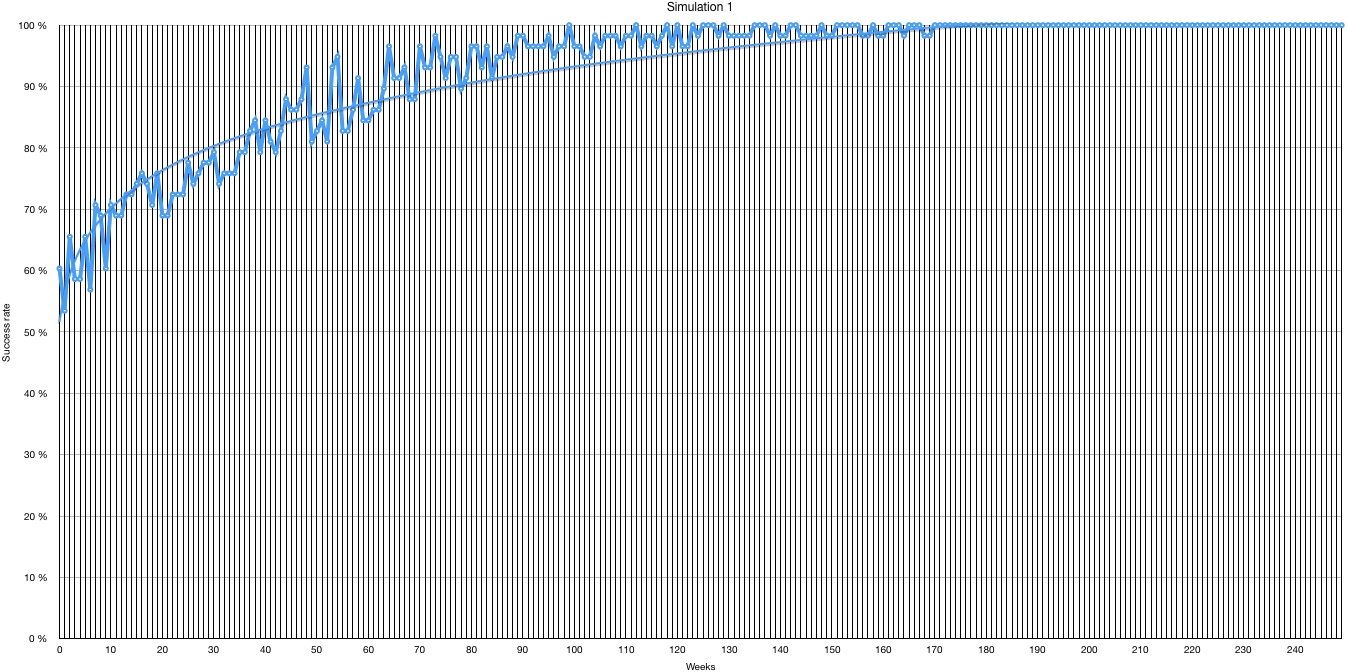
\includegraphics[width=.9\columnwidth]{./Abbildungen/Kapitel_04/sim1.png}
	\caption{Simulation 1: Lernkurve}
	\label{img:sim1}
\end{figure}


\begin{figure}[th!]
	\centering
	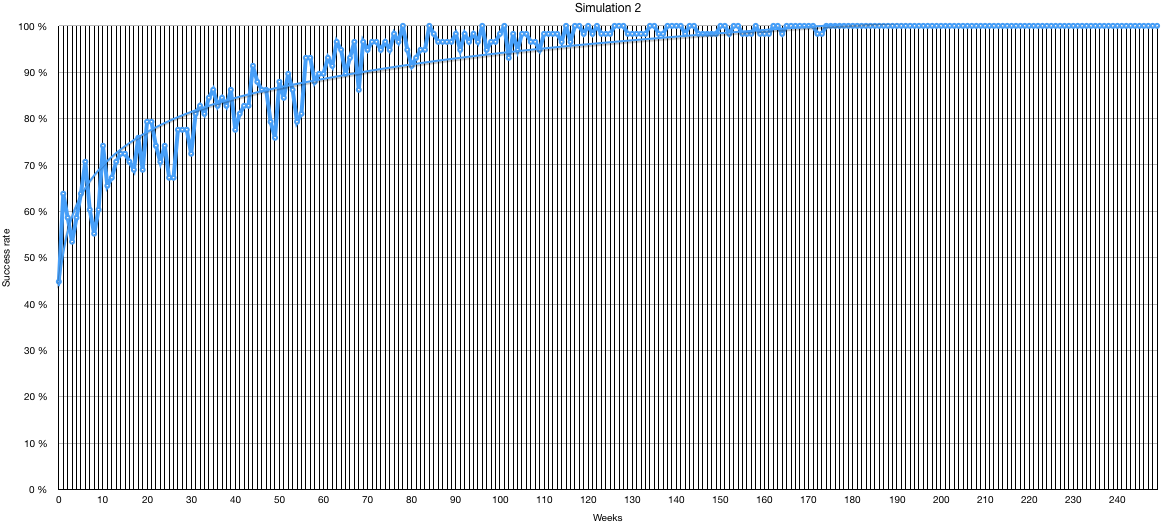
\includegraphics[width=.9\columnwidth]{./Abbildungen/Kapitel_04/sim2.png}
	\caption{Simulation 2: Lernkurve}
	\label{img:sim2}
\end{figure}


\nlparagraph{Simulation 2}
Der Graph der 2. Simulation (vgl. Abbildung \ref{img:sim2}) ist dem der Ersten äußerst ähnlich. So nähert sich dieser dem Optimum auch logarithmisch an und erreicht eine 100\textit{\%} \quotes{success rate} bei ca. 170 Episoden.\\
Aufgrund des sehr hohen Grads der Ähnlichkeit beider Graphen, wird hier auf eine weitere Interpretationen des Verlaufs verzichtet. \\
So sollen lediglich die Ergebnisse der ersten Simulation nochmals untermauert und die einwandfrei Funktionalität der Implementierung des Q-Learning Algorithmus gezeigt werden. 

\nlparagraph{Testphase}
Unter Berücksichtigung der in \ref{sec:testphase} geschilderten Probleme, gilt der Hinweis, dass während der Testphase nur sehr kleine Datensätze für die Evaluation erzeugt wurden. Dadurch erfolgt die Beantwortung der Forschungsfrage nur anhand von abgeleiteten Tendenzen aus den Datensätzen und lässt einen vollständigen Beweis außen vor.  \\
Aus den fünf vorhandenen Datensätzen wurden jeweils zwei zur Auswertung herangezogen, bei denen am häufigsten Feedback durch den User gegeben wurde.\\

\begin{figure}[t!]
    \centering
    \parbox{6cm}{
    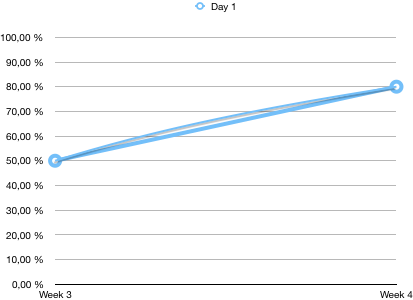
\includegraphics[width=6cm]{./Abbildungen/Kapitel_04/usr1day1.png}
    \caption{User 1: \\Montag}
    \label{img:usr1day1}}
    \qquad
    \begin{minipage}{6cm}
    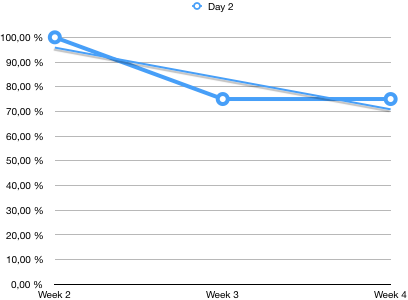
\includegraphics[width=6cm]{./Abbildungen/Kapitel_04/usr1day2.png}
    \caption{User 1: \\Dienstag}
    \label{img:usr1day2}
    \end{minipage}
\end{figure}


\begin{figure}[t!]
    \centering
    \parbox{6cm}{
    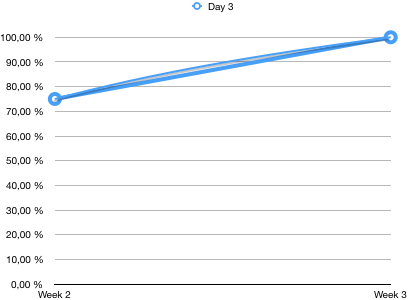
\includegraphics[width=6cm]{./Abbildungen/Kapitel_04/usr1day3.png}
    \caption{User 1: \\Mittwoch}
    \label{img:usr1day3}}
    \qquad
    \begin{minipage}{6cm}
    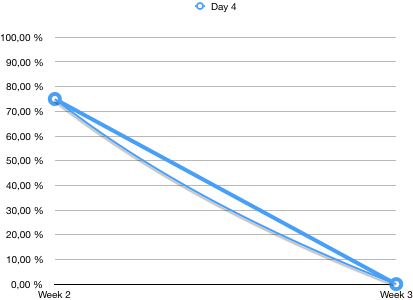
\includegraphics[width=6cm]{./Abbildungen/Kapitel_04/usr1day4.png}
    \caption{User 1: \\Donnerstag}
    \label{img:usr1day4}
    \end{minipage}
\end{figure}

\nlparagraph{User 1}
User 1 wurde erst in der zweiten Woche aktiv, weswegen die Teilnahmedauer nur 2,5 Wochen betrug. 
Betrachtet man den Graphen des Wochenüberlicks (vgl. Abbildung \ref{img:usr1wa}), startet dieser bei einer Erfolgsrate von 75\textit{\%}, fällt in der Woche 3 auf 60\textit{\%} ab und steigt in Woche 4 auf 77,8\textit{\%}. Was daraufhin deutet, dass der Agent aus der Explorationsphase in Woche 3 neues Wissen schöpfen und in Woche 4 anwenden konnte.\\
In Anbetracht der Tagesgraphen, ist im Falle von 3 Tagen (Montag, Mittwoch, Freitag; vgl. \cref{img:usr1day1,img:usr1day3,img:usr1day5}) ein Anstieg der Erfolgsrate um ca. 30\textit{\%} zu erkennen. \\
Der enorme Einbruch an Tag 4 (vgl. Abbildung \ref{img:usr1day4}) von 75\textit{\%} auf 0\textit{\%}, schließt auf ein zur Vorwoche stark verändertes Verhalten des Users. Auch eine Explorationsphase wäre theoretisch denkbar, ist statistisch aber eher unwahrscheinlich.\\
Trotz der Reduktion der Prediction accuracy an Tag 2 (vgl. Abbildung \ref{img:usr1day2}), liegt die Erfolgsrate immer noch bei 70\textit{\%}, was definitiv ein Indiz für den Lernerfolg des Agenten ist. 


\begin{figure}[t!]
    \centering
    \parbox{6cm}{
    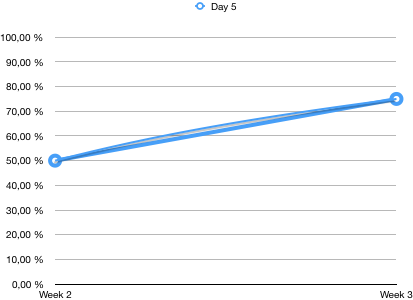
\includegraphics[width=6cm]{./Abbildungen/Kapitel_04/usr1day5.png}
    \caption{User 1: \\Freitag}
    \label{img:usr1day5}}
    \qquad
    \begin{minipage}{6cm}
    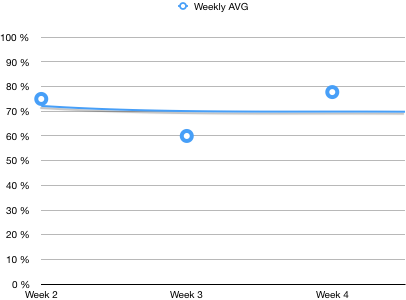
\includegraphics[width=6cm]{./Abbildungen/Kapitel_04/usr1wa.png}
    \caption{User 1: \\Wochenüberlick}
    \label{img:usr1wa}
    \end{minipage}
\end{figure}
    


\clearpage
\newpage

\nlparagraph{User 2}
User 2 war drei Wochen aktiv und startete am 4. Tag der ersten Woche.
Beim Wochenüberblick (vgl. \ref{img:usr2wa}) ist in den Wochen 1-3 zuerst ein Anstieg von 55\textit{\%} auf 68\textit{\%} zu erkennen, welchem anschließend ein Abfall auf eine Erfolgsrate von 44\textit{\%} folgt. \\
Bis auf den dritten Tag ist in allen anderen Fällen (vgl. Abbildung \cref{img:usr2day1,img:usr2day2,img:usr2day4,img:usr2day5})  mindestens einmal ein Anstieg der Erfolgsrate im Vergleich zur Vorwoche zu beobachten. Gerade der Graph des dritten Tages (vgl. Abbildung \ref{img:usr2day3}), bei welchem eine Stagnation über alle 3 Wochen hinweg zu erkennen ist, deutet einerseits auf einen gewissen Lernerfolg hin, zeugt aber auch andererseits von einer fehlenden Exploration des Agenten. \\
Es lässt sich sowohl an den Tagesgraphen, als auch am Wochengraph ein Trend hin zum Lernerfolg des Agenten beobachten. So ist die \quotes{prediction accuracy} in keinem Tag bei 0\textit{\%} und es ist stets ein Anstieg oder zumindest eine Stagnation zu beobachten, was letztendlich auf einen Lernerfolg des Agenten hindeutet.
\\\\
In Anbetracht beider Simulationsergebnisse ist der Lernerfolg bei dieser Problemstellung von logarithmischer Natur. Sowohl der Auswertungsgraph von User 1 (vgl. Abbildung \ref{img:usr1wa}) als auch von User 2 (vgl. Abbildung \ref{img:usr2wa}) teilen diese Charakteristik und zeigen eine Tendenz hin zu einer steigenden Erfolgsrate. Dies würde vorerst die These bestätigen, dass sich Machine Learning und Blockchain verbinden lässt, bzw. das Lernen anhand von Daten einer Blockchain möglich ist. \\
Jedoch muss dies gewissermaßen auch relativiert werden, da die Dauer der Studie sehr kurz war. Die Ergebnisse können eben nur eine Tendenz geben, inwiefern bei einer längeren Dauer der Testphase der Lernerfolg im selben Maße ausfallen würde, wie im Falle der Simulation. \\\\
Schlussendlich bedarf es einer weitaus längeren Studiendauer, um die Forschungsfrage in voller Gänze zu erörtern. 

\begin{figure}[t!]
    \centering
    \parbox{6cm}{
    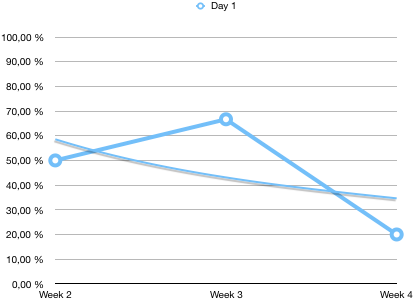
\includegraphics[width=6cm]{./Abbildungen/Kapitel_04/usr2day1.png}
    \caption{User 2: \\Montag}
    \label{img:usr2day1}}
    \qquad
    \begin{minipage}{6cm}
    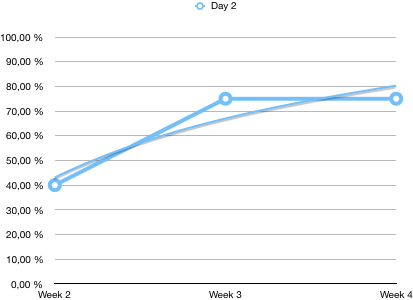
\includegraphics[width=6cm]{./Abbildungen/Kapitel_04/usr2day2.png}
    \caption{User 2: \\Dienstag}
    \label{img:usr2day2}
    \end{minipage}
\end{figure}


\begin{figure}[t!]
    \centering
    \parbox{6cm}{
    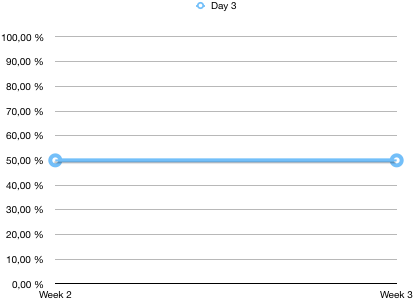
\includegraphics[width=6cm]{./Abbildungen/Kapitel_04/usr2day3.png}
    \caption{User 2: \\Mittwoch}
    \label{img:usr2day3}}
    \qquad
    \begin{minipage}{6cm}
    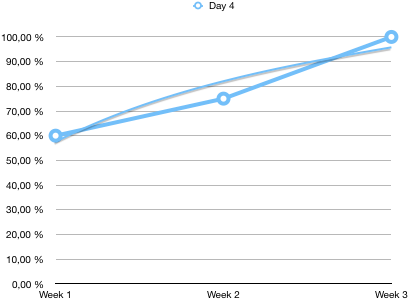
\includegraphics[width=6cm]{./Abbildungen/Kapitel_04/usr2day4.png}
    \caption{User 2: \\Donnerstag}
    \label{img:usr2day4}
    \end{minipage}
\end{figure}

\begin{figure}[t!]
    \centering
    \parbox{6cm}{
    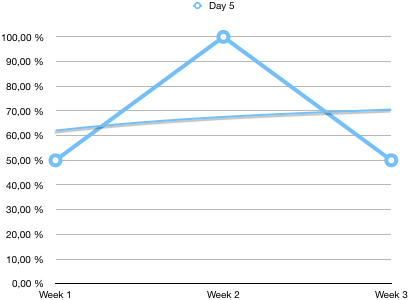
\includegraphics[width=6cm]{./Abbildungen/Kapitel_04/usr2day5.png}
    \caption{User 2: \\Freitag}
    \label{img:usr2day5}}
    \qquad
    \begin{minipage}{6cm}
    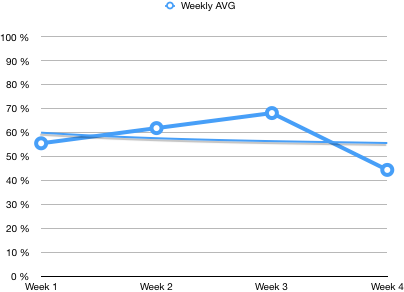
\includegraphics[width=6cm]{./Abbildungen/Kapitel_04/usr2wa.png}
    \caption{User 2: \\Wochenüberlick}
    \label{img:usr2wa}
    \end{minipage}
\end{figure}

\chapter{Zusammenfassung}
\label{kap:Kapitel05}
%
\section{Weiterf\"uhrende Forschungsfragen}
%
\begin{itemize}
    \item anderer algorithmus sarsa
    \item Decision Trees besseres ergebnis?
    \item offline learning from bchain logs --> reinforcement oder unsupervised
    \item algorithmus daten auch auf bchain speichern --> transparenz
    \item 
\end{itemize}
%
\section{Ausblick}
%

%



\pagenumbering{Roman}
	
									
\bibliography{Literatur/Literatur} 	% Literaturverzeichnis
\listoffigures											% Abbildungsverzeichnis
\listoftables												% Tabellenverzeichnis
%\listof{algorithm}{Pseudocodeverzeichnis}

%\printglossary[title=Glossar] 			% Glossar Einträge in Header/Glossar.tex vornehmen
%\printglossary[type=\acronymtype,title=Abk\"urzungsverzeichnis]	% Abkürzungsverzeichnis Einträge in Header/Abkuerzungen vornehmen

\appendix
\chapter{Anhang A}
\label{kap:AppendixA}

\chapter{Anhang B}
\label{kap:AppendixB}


\pagestyle{empty}
%\chapter*{Eidesstattliche Erkl\"arung}
\label{sec:EidesstattlicheErkl�rung}

%Ich versichere, dass die Masterarbeit mit dem Titel \glqq{}\titel{}\grqq{} nicht anderweitig als Pr�fungsleistung verwendet wurde und diese Masterarbeit noch nicht ver�ffentlicht worden ist. Die hier vorgelegte Masterarbeit habe ich selbstst�ndig und ohne fremde Hilfe abgefasst. Ich habe keine anderen Quellen und Hilfsmittel als die angegebenen benutzt. Diesen Werken w�rtlich oder sinngem�� entnommene Stellen habe ich als solche gekennzeichnet.
%\vfill

%\begin{center}
%\begin{minipage}{0.9\textwidth}
%Augsburg, den \today \hfill  Unterschrift
%\end{minipage}
%\end{center}


\end{document} 